
\graphicspath{{ChapterSrep/images/}}
\chapter{3D object representation}
\label{chapter:3DModels}

\section{Introduction}
\label{sec:3DModels}

Advances in technology have made possible to 
develop high quality 3D models that are used in various
sectors of the industry.
They implement a mathematical description of the appearance of the object
that can be used for animation, prototyping and simulation purposes. 
The geometry of the object is the core of these procedures.

Today's challenge is to create models of objects that are adapted 
to perform robust simulation procedures. 
They should provide the mechanisms to include information from 
various sources at different spatial scales and
also work in multi-object scenarios.
Moreover, their shape must be representative of a population, 
implying the establishment of a methodology to compute mean shapes 
and a description of the variability in the population. 
There is no standard technique to 
deal with shape, nor to compute average shapes.
Those are rather challenging tasks in computer vision.
%In a generalized manner there should be more efforts to understand
%how the mechanisms of human perception 
%deal with shape as they do it very well but they are not completely understood. 

Developing a model with the characteristics stated above 
opens the possibility to improve existing simulation procedures,
acquire a better understanding of the systems in the human body,
develop better automated analysis on medical images and
also improve personalized medicine.
Furthermore, (non-invasive) medical interventions could be planned using
patient specific models since they are created from 
the information acquired on the medical images.

A review of state of the art techniques to improve 3D modeling of organs
is done in the following section. 3D modeling can be divided broadly 
into two categories: surface modeling and solid modeling.

Surface models represent only the outer layer of the object. They are stored 
as a set of primitives such as points, edges or polygons and define the boundary of the object.
During the last 20 years, most of the research has been focused on this category as they are easier to manipulate.
Surface modeling can be divided into different sub-categories: landmark representations and
boundary representations or b-reps. 

Solid models on the other hand represent both, the exterior and the interior of the object. 
They can be divided mainly into two sub-categories: atlas based deformable models and quasi medial-representations. 
%Unfortunately, solid models require more computational power and have been used mostly for research purposes.

The chapter is organized as follows, Section \ref{sec:surfaceRep} gives an overview of the most important surface modeling
techniques, Section \ref{sec:solidRep} gives an overview of solid modeling techniques with emphasis on s-reps, 
the technique that I will be using throughout this dissertation. 
My contribution to s-reps are a new interpolation method based on splines, which will be explained 
in Section \ref{sec:s-repImplementation}.
Section \ref{sec:3dRepConclusion} gives a conclusion of the methods.


\section{Surface representation}
\label{sec:surfaceRep}


Surface representation techniques can be divided 
broadly into two categories: landmark representations and boundary representation or b-reps. 
I overview the most prominent authors in the following section.


\subsection{Landmark representations}

Landmark representations were proposed by \cite{kendall1989survey}. 
Since landmark representation is a simple method to perform shape analysis,
there has been an extensive study of their geometry and statistics \cite{bookstein1991morphometric}, \cite{dryden1993multivariate}, \cite{james1993revolution}, \cite{small1996statistical}.

Kendall understood shape as a set of prominent features (landmarks) in the objects and gave the following definition: 

\begin{definition}
 \label{def:shape}
 \textit{Shape} is all the geometrical information that remains when
 a specified group of transformations are filtered from the object. That group consits of translations, rotations and scaling.
\end{definition}
 
This filtering is accomplished by Procrustes analysis. 

Procrustes analysis is done to match the landmarks 
by putting them on a common frame and derive valid information 
from their displacement. 
This is equivalent to understanding how the shape deforms
on the population. 

I will briefly describe how a Procrustes analysis is done.
To filter the location, the object must be centered on its geometric center or centroid.
Let $O = \{x_i: i < k, k \in N\} \in R^n$ be the set of landmarks that compose an object.
The centroid of $O$ is defined in Equation \ref{equ:centroid}. 

\begin{equation}
  C(O) = \frac{\sum_i^k O(i)}{k}
  \label{equ:centroid}
\end{equation}

The object is then translated by $C(O)$ i.e., $O_t = \{x_i - C(O): i < k, k \in N\} \in R^n$.
We will see in Section \ref{sec:medialRepresentations} that in some cases, centering at the centroid 
is not adequate to perform shape analysis.

To filter the scale or make $O$ unit scale, the object is normalized.
Scale is defined as a linear transformation that enlarges or shrinks an object.
To remove the scale of an object the root mean square distance from the points to the centroid must be equal to 1.
The calculation of this coefficient is defined in Equation \ref{equ:norm}.

\begin{equation}
 N(O) = \sqrt{\frac{\sum_i^k (O(i) - C(O))^2}{k}}  
 \label{equ:norm}
\end{equation}

The object $O$ is scaled by $1/N(O)$: $O_s = \{O(i)/N(O): i < k, k \in N\} \in R^n$.

The last step is to filter the rotation, 
which is defined as moving an object around a point or axis of rotation, as shown in figure \ref{fig:Rotation}.
In this example, the object is rotated $45^o$ clockwise and the axis of rotation
is the crossproduct between the $x$ and $y$ axes.

\begin{figure} 
 \centering 
 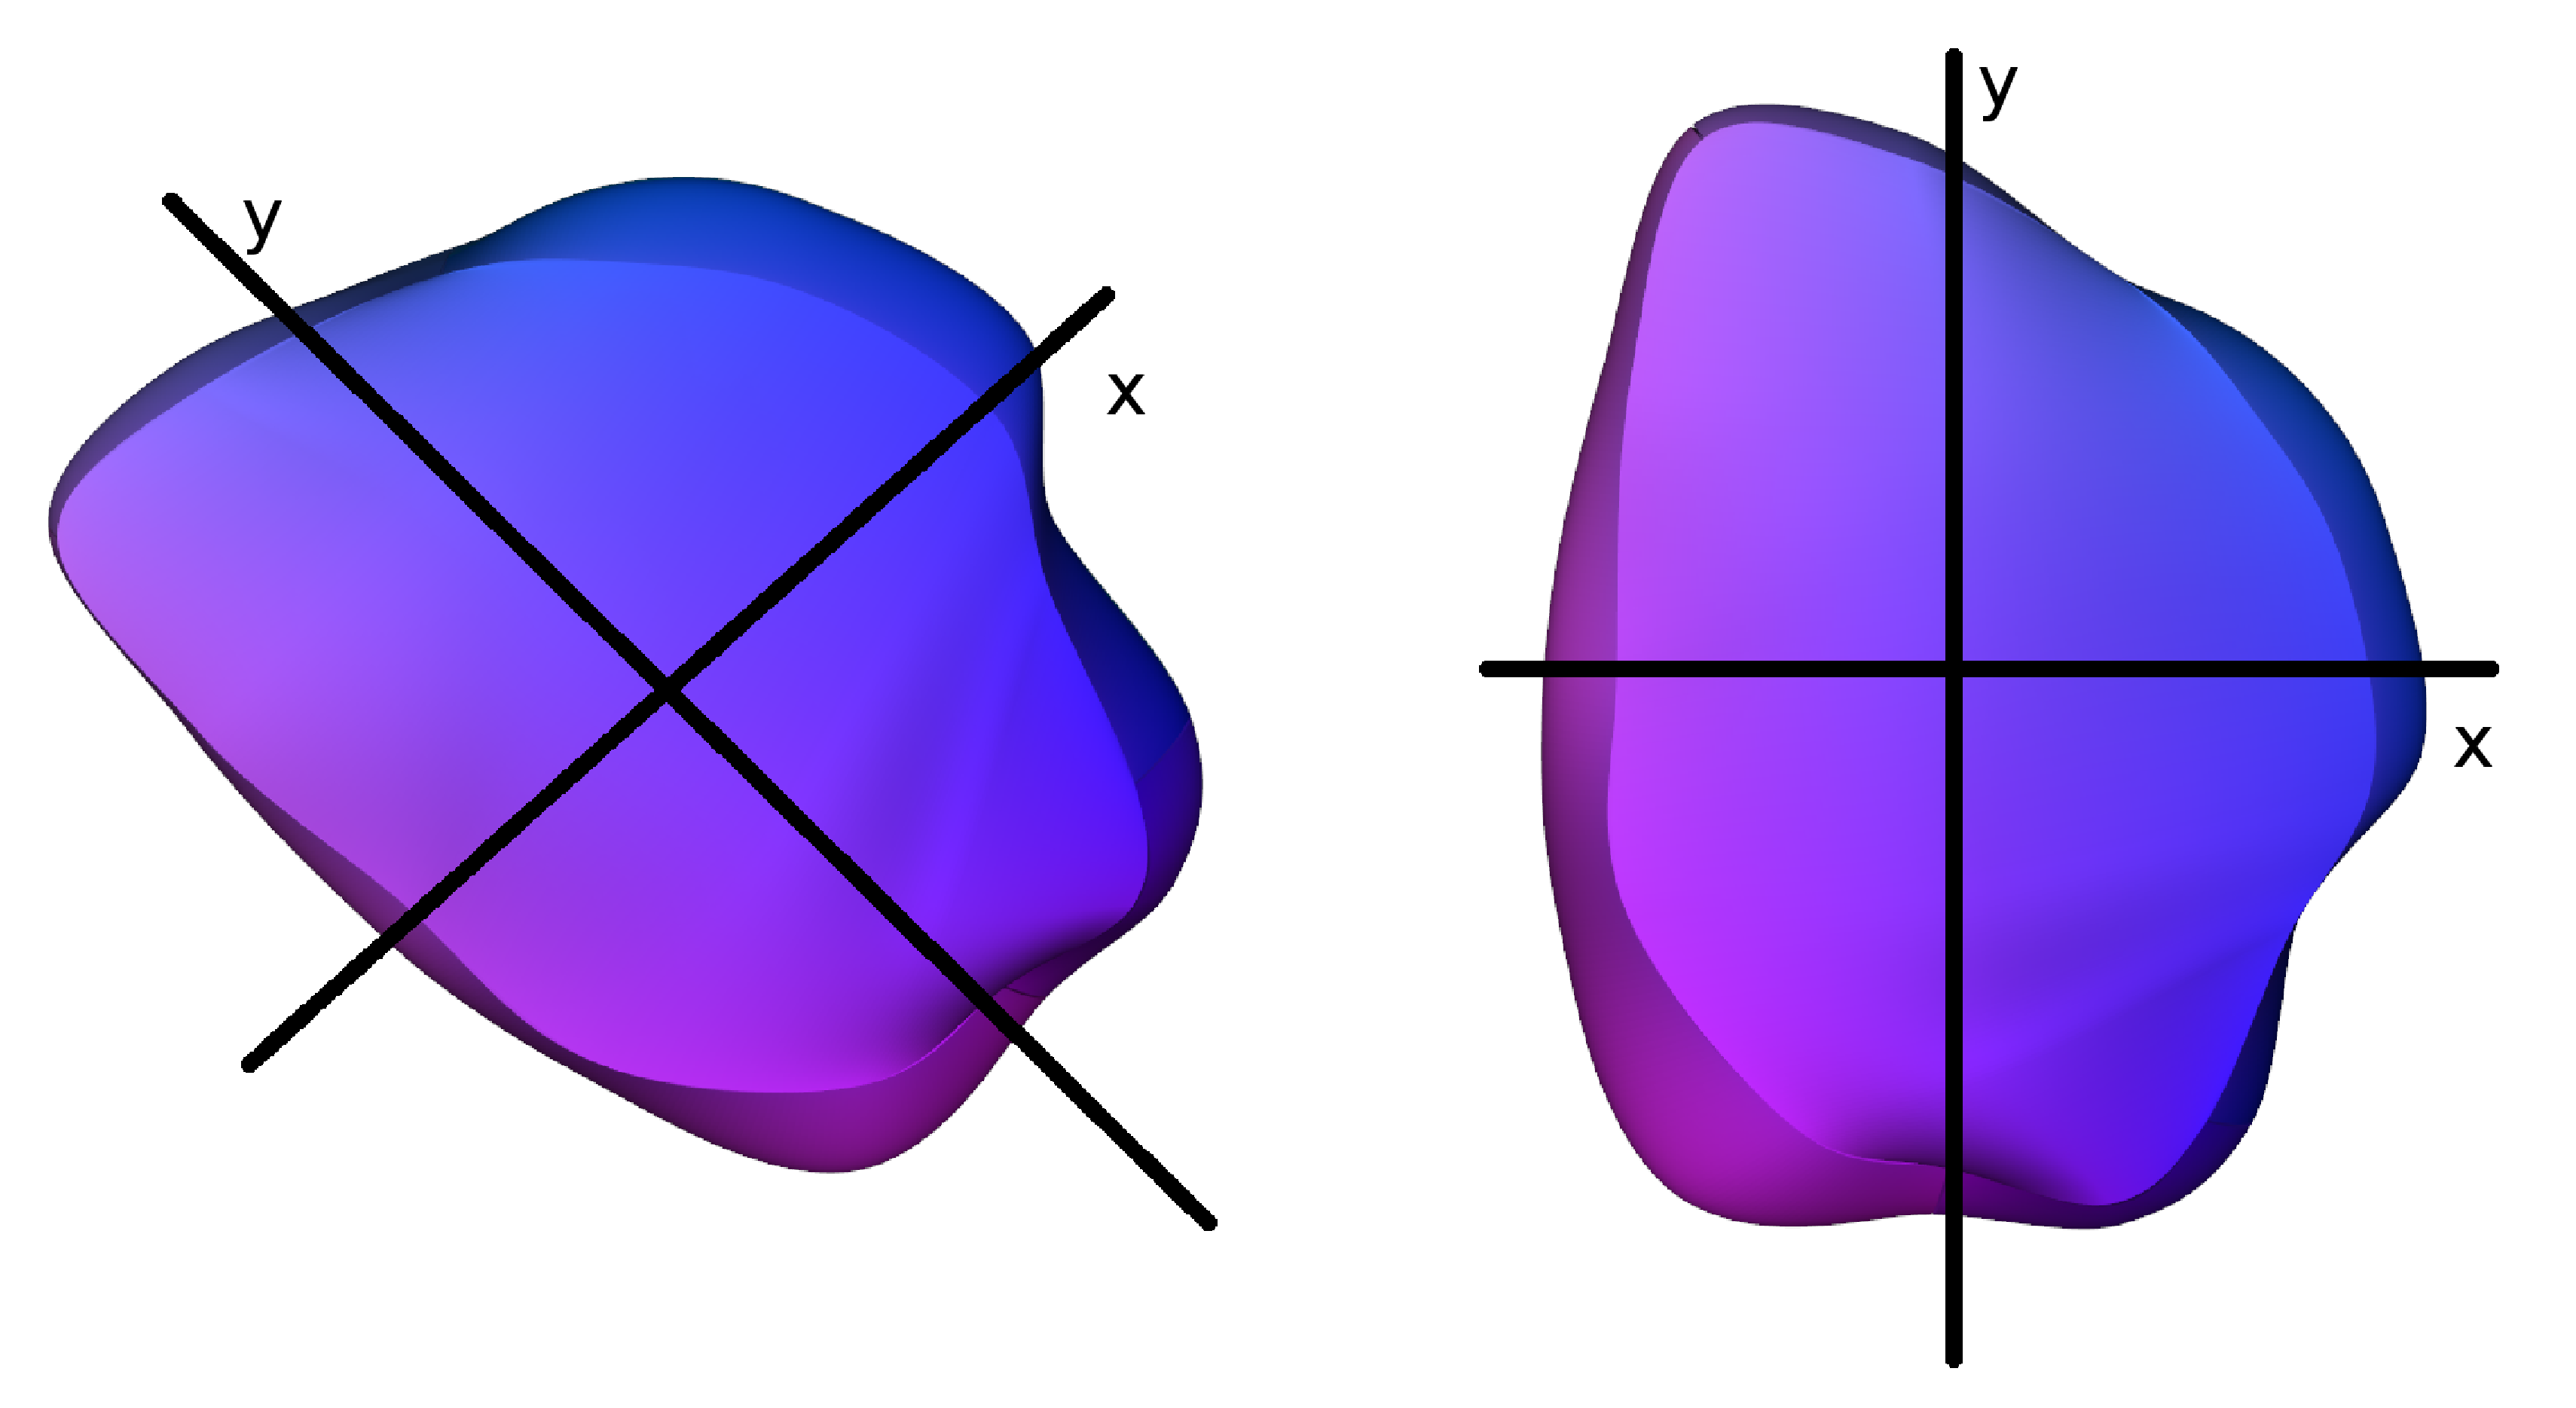
\epsfig{file = rotation.eps, width = 8cm}
 \caption[Rotated figure.]{Figure rotated 45 degrees clockwise.}
 \label{fig:Rotation}  
\end{figure}

Since a rotation can be expressed in matrix form,
the alignment problem can be done 
iteratively by minimizing the distance from the points 
in two objects as shown in Equation \ref{equ:align1}.

\begin{eqnarray}
  [\hat{\Omega}] = \operatorname*{arg\,min}_{\Omega} || \Omega O_i - TO_i||
  \label{equ:align1}
\end{eqnarray}
where $\Omega$ is a rotation matrix around the centroid of the object.
$O$ is an object and $TO$ is a target object or template where both objects are centered on the origin and have unit scale.
The problem consists in finding a matrix $\Omega$ such that the distance from points in $O$ is minimum
to the points in $TO$.

Using matched landmarks 
in a population of objects, this enables the study of shape by 
analyzing the displacements of the landmarks from the target to each object across the population. 

Further improvements of landmark representations sought to produce constrained diffeomorphic deformations i.e., 
differentiable maps that have a differentiable inverse. 
Without the constraint, mapping an unfolded template to a folded structure 
produces non diffeomorphic defformation and
causes to lose the geometry and topology of the template.

\cite{joshi2000landmark} associated the transformation with an energy term,
forcing the existence and uniqueness of the solution, 
thus, enabling the creation of smooth differentiable maps.
This causes the landmarks to deform correctly to the target object and preserve the topology even if 
it is curved. 

Although landmark matching performs well in the study of biological shape and
is able to compute statistics from landmark displacements that 
capture information on scale, translation, rotation and shear.
Information on bending, widening and elongation 
are not very well captured by the approach.
Another major drawback is on landmark positioning.
This is usually done by hand, which is time consuming. 

\subsection{Boundary representations} 

Boundary representation include the following approaches: active contours, active shape/appearance models and projection onto orthogonal functions.

\subsubsection{Active contours} 

Active contours is a method proposed by \cite{kass1988snakes}, commonly known as snakes.
The method was conceived mainly for image segmentation procedures based on curve evolution.

It starts with the definition of a contour $V$ composed by a set of points $p_i$ and an energy function defined for $V$. 
The function has two components corresponding to the internal and external energy in the object being segmented or geometric typicality and
an image match term as defined in Equation \ref{equ:snake}. 

The geometric typicality is responsible for the smoothness of $V$ and its propagation in a desired direction.
Smoothness is controlled by $Econtinuity$ and the direction of propagation by $Eballoon$, ensuring that
the snake curve keeps propagating in the desired direction. 

The image match term takes into consideration the intensity pattern around each vertex $p_i \in V$.
$Eintensity$ makes $V$ move to a region of low or high image intensity information and 
$Egradient$ attracts $V$ to the edges of the object being segmented. 
The whole energy of the contour is defined by the integral in Equation \ref{equ:snakeEnergy}.

\begin{eqnarray} 
 E(V(s)) = \alpha Eint(V(s)) + \beta Eext (V(s)) ds\\
 Eint (V) = \gamma Econtinuity (V) + \delta Eballoon (V)\\
 Eext (V) = \eta Eintensity (V) + \varphi Egradient (V)
 \label{equ:snake}
\end{eqnarray}

\begin{equation}
 E_{snake} = \int_0^1 E(V(s)) ds\\
 \label{equ:snakeEnergy}
\end{equation}

\begin{figure} 
 \centering 
 \epsfig{file = snakes.eps, width = 8cm}
 \caption[Snake's energy.]{Image taken from \cite{kass1988snakes}. The contour moves back to the edge of the pear.}
 \label{fig:snakes}  
\end{figure}

As shown in Figure \ref{fig:snakes}, the contour maps back to the edge of the pear after the perturbation; 
this place is where the minimum is found.

Two major drawbacks of the active contour model are in the initialization step 
since the countour must be placed according to the object being segmented, 
and the need for the boundaries of the object to be defined by a gradient, i.e., to have a smooth boundary with contrast everywhere. 

\cite{chan2001active} proposed an active contour model based on the segmentation 
techniques by \cite{mumford1989optimal} and the level set method. 
The level-set method 
models the internal information of an object.
An example of a level set method is the DT (distance transform).
The DT labels each pixel in the image with the distance value to the nearest boundary point, 
having $0$ at the boundary and either positive or negative in the interior and exterior of the object. 
Even though this information could be 
used to locate and reference the position of internal features in the object, 
the information is only used to 
produce boundary segmentations 
or in other words, to model the curve/surface propagation flow until reaching a stable position.

Figure \ref{fig:chanveseS} shows the automatic segmentation of an object whose boundaries are not well defined and 
the contour can be place anywhere in the image.

\begin{figure} 
 \centering 
 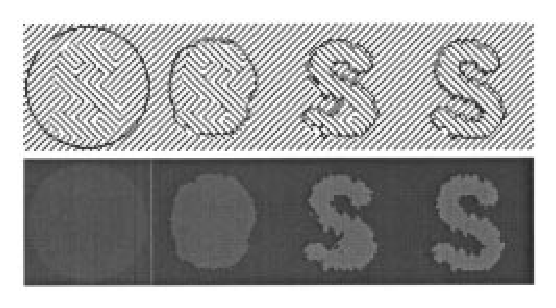
\epsfig{file = chanVeseS.eps, width = 8cm}
 \caption[Segmentation with orientation.]{Image taken from \cite{chan2001active}. The contour of 'S' is not well defined, the segmentation succeeds due to the grouping based on orientation identity.}
 \label{fig:chanveseS}  
\end{figure}

In some situations the regions that are being segmented could be divided, due to high noise on the image or occlusion.
To solve this problem, \cite{jeanvariational} proposed a region growing approach that includes
different type of descriptors in the minimization process.

The approach defines regions in the image via a discrete function:

\begin{equation}
  \phi^{n}(x) =  \begin{cases}
			   1, \text{for $x$ } \in \Omega_{in} \\
			   0, \text{for $x$ } \in \Omega_{out}, 
		 \end{cases} 
   \label{equ:vrgRose}
\end{equation}
where $\Omega_{in}$ and $\Omega_{out}$ are the regions that correspond to the segmented pixels.
The regions defined in $\Omega$, change according to the region-based energy $J(\phi^{n})$, which must
be designed so that its minimum corresponds to the expected solution. At each iteration $n$, the voxels that are connected to $\Omega_{in}$
are tested. If the addition of those voxels decreases the energy, then, they are accepted and the discrete function is updated as

\begin{equation}
 \phi^{n+1}(x) = \frac{1}{2}(1-sign\left(\Delta J(\phi^{n+1})\right).
\end{equation}

This approach has been tested in segmentation of the vascular tree in the lung as shown by \cite{PRIE-12c}, \cite{PRIE-12e}.
The descriptors used on the images are based on a vesselness criterion proposed by \cite{springerlink:10.1007/BFb0029240} and on the gray levels of the original image.
The objective is to detect tubular structures in the image.

The complete formulation using the vesselness descriptors is as follows:
\begin{equation}
  \Delta{J(\phi^{n+1})} = 1 - 2\phi^{n}\left(\Delta{J_{1}}(f, v)\right),
\end{equation}
\begin{equation}
  \Delta{J_{1}}(f, v) = \begin{array}{l}
                         \frac{v}{MaxV} \left( |v - \mu_{v_{in}}|^2 - |v - \mu_{v_{out}}|^2 \right)   \\
			+  \left|\frac{f}{MaxF}\right| \left(|f - \mu_{f_{in}}|^2 - |f - \mu_{f_{out}}|^2 \right),
                        \end{array}
\end{equation}
where $MaxV$ is the maximum value of the vesselness criterion, $\mu_{v_{in}}$ and $\mu_{v_{out}}$ 
are the mean values of the vesselness image voxels in $\Omega_{in}$ and $\Omega_{out}$ respectively. 
$MaxF$ is the maximum value in the original image, and similarly $\mu_{f_{in}}$ and $\mu_{f_{out}}$ are the respective mean values in the image 
for the regions $\Omega_{in}$ and $\Omega_{out}$.

After the segmentation is done by any of the curve evolution methods stated above, 
the user is left with a set of points that correspond to the boundary of the object. 
Once again, notice that the approaches lack the mechanisms to describe internal features of the objects.

The following section introduces segmentation using combined geometric and intensity models, know as active shape and appearance models. 

\subsubsection{Active shape and appearance models} 

ASM (Active shape models) was proposed by \cite{cootes1995active}. 
The approach is based on the formulation that complex images can be analyzed by using 
shape priors. 
It differs from previous approaches that search to segment structures based 
on edges or homogeneous regions by introducing a deformable model template of the
objects that exist in the image. 

A deformable template is defined as proposed by \cite{fisker2000making}:

\begin{definition}
  A \textbf{deformable template} model can be characterized as a model, which under an implicit or explicit optimization
  criterion, deforms a shape to match a known type of object in an image. 
\end{definition}

The segmentation procedure uses the deformable template 
and tries to minimize an energy function that matches the template 
on the image.
In general terms, the approach could be described as observe, learn and match.

The observation stage consists in generating the set of 
training cases. To do this, each object or structure of interest is
represented by a set of points or landmarks. These points can represent
the boundary and internal or external features. 
For each case, the points are required to be 
placed in the same manner. This task 
is usually performed by hand and validated by an expert. 
Although automatic methods have been proposed to speed up the process \cite{hill2000framework}, \cite{heimann2007shape},
the outputs are often revised and corrected. 

Once the landmarks are placed on each training case, they are aligned to a common set of axes.
Recall that if the cases are not aligned, the statistics are meaningless.

After the alignment, the learning stage is done using PCA (principal component analysis); see Appendix \ref{sec:apendixPCA} for details.
PCA detects salient features or principal directions of variation,
removes redundant information and produces a compact representation of the data.

Once the principal direction of variation is detected in the population, 
any of the training sets in the data can be approximated using
\begin{equation}
 x_i \approx Pb + \bar{x}
 \label{equ:approxData}
\end{equation}
where $P = (p_1 |p_2 | . . . |p_n )$ contains $n$ eigenvectors (produced by PCA)
and $b$ is a $n$ dimensional vector that defines a set of 
parameters of a deformable model. 

The variance of the $i_{th}$ parameter of $b_i$ across the training set is given by $\lambda_i$. By applying limits
$\pm 3 \sqrt{\lambda_i}$ the resulting model is guaranteed to be in the population. 

The final stage is to match a new input to the training cases.
This could be done in an iterative process. 
Using the alignment explained in section \ref{sec:surfaceRep},
the matching of a new object $x_i$ goes as follows: 

\begin{enumerate}
 \item Initialize $b$ to zero.
 \item Generate a model $y$ using Equation \ref{equ:approxData} and appearance information.
 \item Align $y$ to $x_i$ using the transformation $\Gamma$ given by Equation \ref{equ:align1}.
 \item Project $x_i$ into model coordinates using $\Gamma^{-1}$, $x_i' = \Gamma^{-1}(x_i)$.
 \item Project $x_i'$ into the tangent plane to $\bar{x}$ by scaling: $x_i'' = x_i'/(x_i' \cdot \bar{x})$
 \item Update $b = P^T (x_i'' - \bar{x})$
 \item Repeat from 2 until convergence.
\end{enumerate}

This general approach to match shape has proven to be very effective in image segmentation. 
It has been applied in applications such as object tracking, detection and recognition.

The AAM (Active Appearance Model) proposed by \cite{cootes2001active} improves the ASM by learning image appearance
statistics as well as the location 
of the landmarks, i.e., each appearance vector is built from the image intensities (grey level or multiple components as RGB).
PCA is applied separately on the landmark information of appearance and location.

A third PCA is applied to search for correlation between the shape and appearance analysis. 
This final PCA is the one used to produce the approximations of a new model.

A speed-up of the method was also proposed by \cite{mitchell20023} where the search for the closest model is done in a multi-scale 
fashion. 

In general terms ASM and AAM are robust and efficient methods in image segmentation, 
we will see in section \ref{sec:medialRepresentations} that 
other methods similar to PCA are best suited to produce statistical information for 3D shape analysis.

\subsubsection{Function based models} 

Function based modeling offers great flexibility and precision. 
The key concept is to use a set of smooth functions to approximately model the surface of an object.
One of the strengths of using such functions is that the derivatives of the object's surface are available and 
boundary normals and curvatures can be derived analytically. 
In contrast to PDM (point distribution models such as landmark based or ASM), these methods efficiently represent
a shape model by using fewer parameters.

Different types of functions can be used to reconstruct a surface, including 
orthogonal functions and spline based methods such as NURBS (Non-Uniform Rational Basis Splines).

There are many type of orthogonal functions: spherical wavelets \cite{schroder1995spherical}, 
SPHARM (spherical harmonics \cite{brechbuhler1995parametrization}, 
Hermite polynomials \cite{bradley1997geometric}, among others.

Spherical Wavelets describe surfaces that have spherical topology.
A wavelet is a function that localizes a given function in space and scale.
In other words, wavelets can represent a given function at multiple levels of detail
and in multiple regions. 
They are superior to a conventional Fourier transform
because they capture 
low and high frequency components of the signal at
specific locations in time or space.
Equation \ref{eqn:wavelet} shows the general formula of a wavelet.

\begin{eqnarray}
 \Psi_{a, b}(t) = \frac{1}{\sqrt{a}}\Psi(\frac{t - b}{a}) \\
 x_a(t) = \iint x(t) \Psi_{a, b}(t)dt
 \label{eqn:wavelet}
\end{eqnarray}

To create a spherical wavelet, the shape of the object is mapped onto the sphere,
and a signal is sampled from it \cite{schroder1995spherical}.
The signal is decomposed in various steps of subsampling and differentiating.
At the end, the procedure retains a coarse representation of the sphere. 
To recover the information lost during the sumbsampling of the signal, a Haar-like operator
is used such that it retains the differences between the two stages \cite{schwartz2008tr}.
The wavelet signal can be used for (lossy) signal compression and can be further analyzed
by PCA. The analysis by PCA yields a mean shape that contains global information 
about the population. 
One of the major drawbacks of the approach lies in the fact that they are only able to represent 
objects of spherical topology. 
A second issue is also found for objects that need to be mapped 
on a sphere to produce the transformation. The mapping can introduce undesired distortion. 


SPHARM functions only represent objects with spherical topology. 
This approach starts by unfolding and mapping the object onto a sphere, where each 
point can be expressed by two parameters in spherical coordinates $(\theta, \phi)$. 
An optimization is performed over the projected points that aims to preserve the area of original
surface elements and minimize their distortion. 
Once the spherical parameterization is obtained, 
the surface $\vec{v}(\theta, \phi) = (x(\theta, \phi), y(\theta, \phi), z(\theta, \phi))^T$
can be expressed as
\begin{equation}
 \vec{v}(\theta, \phi) = \sum_{l=0}^\infty \sum_{m=-l}^l \vec{c}_l^m Y_l^m(\theta, \phi)
 \label{equ:sphericalHarmonics}
\end{equation}
where a least-squares procedure 
finds the best coefficients $\vec{c}_l^m$ for the spherical harmonic basis functions $Y_l^m(\theta, \phi)$, 
for a review on spherical harmonic functions see \cite{mohlenkamp2010user}.
Image \ref{fig:spharm} shows a lateral ventricle surface using different harmonics.

\begin{figure} 
 \centering 
 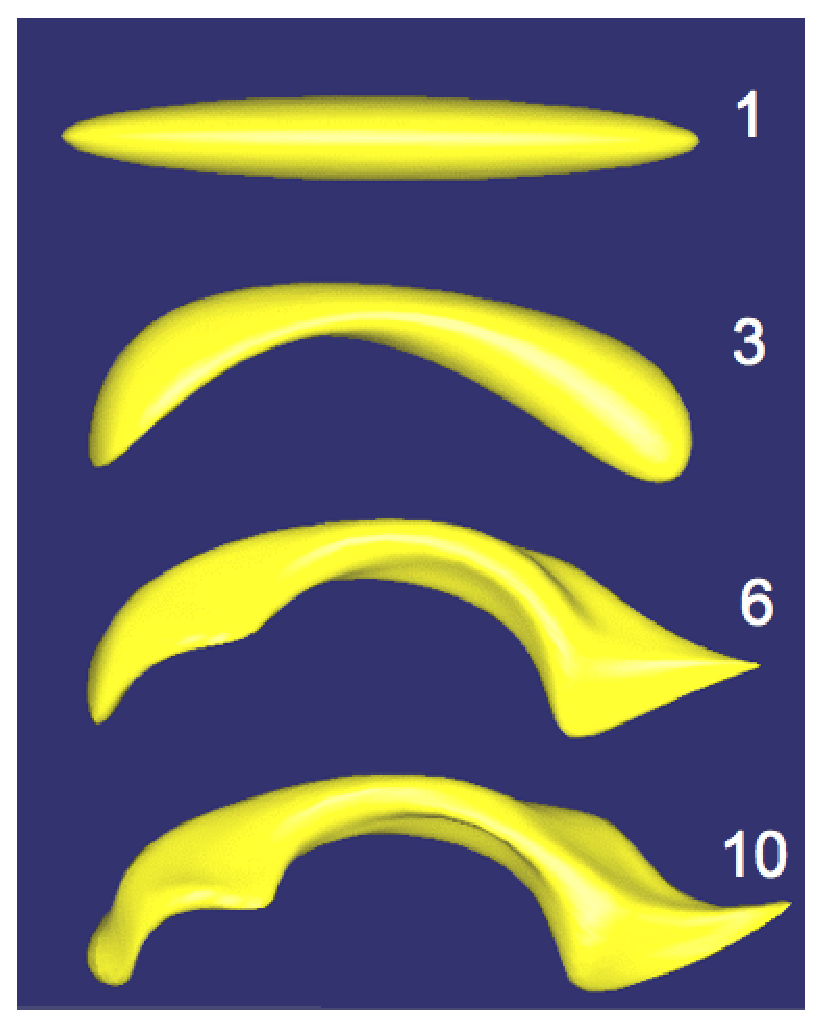
\epsfig{file = spharm.eps, width = 6cm}
 \caption[SPHARM description.]{Image taken from \cite{styner2004boundary}. The SPHARM shape description of a human lateral ventricle 
	  shown at 4 different degrees ( 1, 3, 6, 10 harmonics).
}
 \label{fig:spharm}  
\end{figure}

SPHARM functions were used to estimate the age of a person based on the 
shape analysis of 3D X-ray CT images of human fourth ribs \cite{PRIET-12d}.

Other type of functions can be used to model an object's surface. I am interested in 
the Hermite based functions and spline based methods. They will not be detailed in this section
as they will be reviewed in Section \ref{sec:s-repImplementation}.


\section{Solid representation}
\label{sec:solidRep}

\subsection{Atlas based deformable models}
\label{sec:atlasDeform}

Atlas based deformable models are included in solid representation 
because the geometry of the template (atlas) is well known, 
including its surface and internal features. 

The atlas deformation is based on image registration techniques.
To define image registration, I take the following definition given by \cite{brown1992survey}:

\begin{definition}
 \textbf{Image registration} can be defined as a mapping between two images both
 spatially and with respect to intensity.
\end{definition}

This matching produces deformation maps where every position $p_i$
in the atlas $I_a$ is known on the target $I_t$, therefore 
a registration can be expressed as
\begin{equation}
 I_a(p_i) \approx g(I_t(f(p_i)))
\end{equation}
where $f(p_i)$ is a spatial coordinate transformation
and $g$ is an intensity transformation.

Using the deformation maps, the position of every voxel 
(including internal features) from the atlas can be found on 
the target object. 

To produce the registration, the transformation uses different image descriptors and spatial information. 
The mapping finds an optimal solution, where the optimum depends on the type of descriptors.
For an updated review on image registration techniques see \cite{wyawahare2009image}.

The outputs produced by registration techniques are smooth diffeomorphic maps; 
this means that local structure is also preserved during the deformation \cite{narayanan2005diffeomorphic}. 
For this reason, they have been used to develop transformation-based
probabilistic atlas as shown by \cite{cao2005large} where it describes the variation of ventricular geometry 
and fiber organization (internal features).

Popular software suites for unsupervised segmentation and labeling of structures in the brain
can be found in Freesurfer \cite{fischl2002whole}, \cite{fischl2004automatically} and 
BrainVisa \cite{pohl07_3}. Both are atlas based registration techniques. 

Even though, image registration is known to have to much uncertainty,
it is an approach broadly use for medical image analysis. 
It is difficult to evaluate how well the procedure performs and this is  
a critical point for medical diagnostics, where accuracy is needed. 
Uncertainty arises because the registration produces a single deterministic answer.
Some authors propose solutions to solve this issue by doing posterior statistical analysis 
based on the intensity information \cite{kybic2010bootstrap}, \cite{simonson2011image}.

Measuring uncertainty is helpful to determine whether the results 
can be trusted or not. This measure could possibly be exploited
in unsupervised segmentations or a multi-atlas registration scenario, by giving weights to each atlas based 
on their performance. 
In any case, statistics on deformations are still not adequately developed and remain the major
drawback of the approach. 

The following section is for medial representations, the type of modeling that will be used throughout
this dissertation. 

\subsection{Medial representations}
\label{sec:medialRepresentations}

\begin{chapquote}{Harry Blum}
  For even so simple a notion as location of an object, the contour or perimeter description is particularly poor.
\end{chapquote}

The concept of medial representation started with \cite{blum1967transformation}.
Blum noticed that for any shape, it was possible to calculate a medial axis and 
by doing it, the objects can be described from the inside, in contrast to the techniques 
in Section \ref{sec:surfaceRep}, that seek to model the outside of the object only.

To explain this concept Blum used a grassfire analogy, where the formation of the medial axis is done by setting fire to 
the outer layer of the object i.e., its boundary. The fire propagates uniformly towards the interior of the object and 
when the fronts meet we find the medial axis, a notion related to level-set. 
Following this concept the definition of a medial axis is as follow:

\begin{definition}
 The \textbf{medial axis} is the collection of interior points with at least two closest points on the boundary.
 \label{def:medialAxis}
\end{definition}

In conjunction with the MA (MA will be use to denote medial axis or medial locus similarly) a MAT (medial axis transform) is generated: 

\begin{definition}
 The \textbf{medial axis transform} contains the distance from each point of the medial axis to the boundary of the object. 
\end{definition}

In the context of the grassfire analogy, the MAT adds to each axis point a value equivalent to the burning time from the boundary 
until two fronts meet at the MA.
The MAT has been criticized as small boundary perturbations produce significant changes
on the MA, which yields it impractical for shape description. Figure \ref{fig:unstable} shows 
an example of unstable MA.
This instability has been the focus of many research groups that seek 
to produce a better computation of the MA. 
The idea is to identify the most meaningful 
subsets that compose the MA by trading exactness for stability.

Typically, a pruning of the MA is performed by a threshold value and a criterion that determines
``substance'' and ``connection'', substance being the tangible part of the object and connection, 
how the parts are connected. 
To have a better understanding of this concept think of a complex object such as a hand. 
A hand is compose by a palm (a blob) and fingers (protrusions) or 
think of it as a collection of more complex objects. The substance is
connected in a such a way that we perceive a hand.

\begin{figure} 
 \centering 
 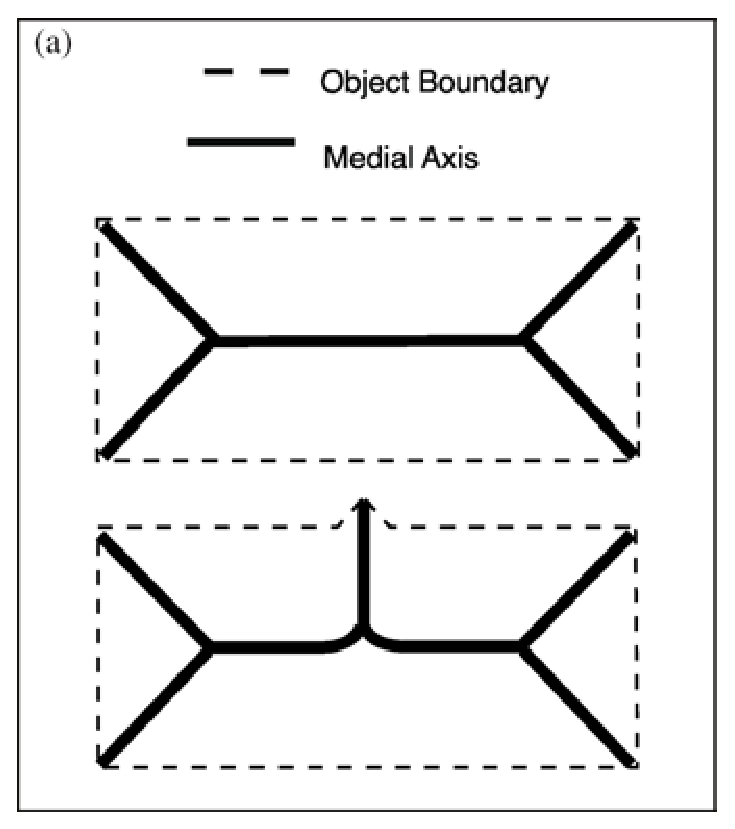
\epsfig{file = medialUnstability.eps, width = 8cm}
 \caption[MAT instabilities.]{Image taken from \cite{katz2003untangling}. MAT instabilities: A tiny change in the boundary produces a large change in the MAT.}
 \label{fig:unstable}  
\end{figure}

Different authors provide the means of computing stable MA: see the methods by
\cite{culver1999accurate}, \cite{amenta2001power}, \cite{katz2003untangling}, \cite{miklos2010discrete}. 

A stable MA is a powerful shape descriptor that
produces compact shape representations of the surface of an object and provides better notions of concepts such as ``center point'' and 
positions inside and relative to the object.
As mentioned in section \ref{sec:surfaceRep} the centroid is used
to align objects on a common frame. In some cases the centroid 
of an object is outside the object itself, thus, making it unsuitable for alignment procedures.
By computing the center point on the MA, it is guaranteed that it will 
be inside the object and its position will be stable under different transformations of the object \cite{liu2011extended}.

The notions such as a position inside the object or relative to other objects are not addressed 
by any of the techniques discussed in Section \ref{sec:surfaceRep}.
These are trivial when an object is described by its MA. 
Positions inside the object will be discussed later in Section \ref{sec:internalCoordinates}.

In 2D the MA is created by computing maximally inscribed discs, with at least two 
points on the boundary. The union of disk's centers form the MA.
In 3D the MA is composed by sheets, generated with maximally inscribed spheres.
In general terms, the MA extends in higher dimensions, where it is composed by hypersurfaces
generated with maximally inscribed hyperspheres.

\begin{figure} 
 \centering 
 \subfigure[Growing]{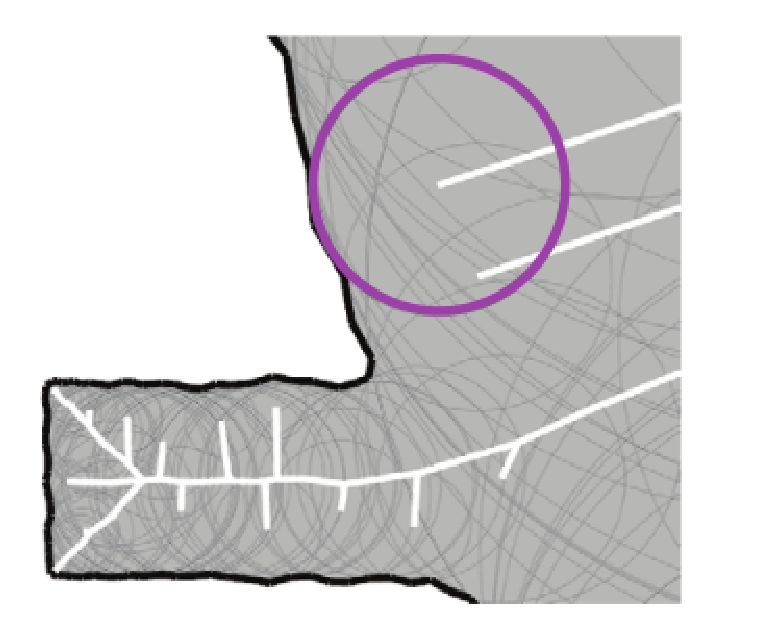
\epsfig{file = StableMedialAxis0.eps, width = 4.5cm}}
 \subfigure[Shrinking]{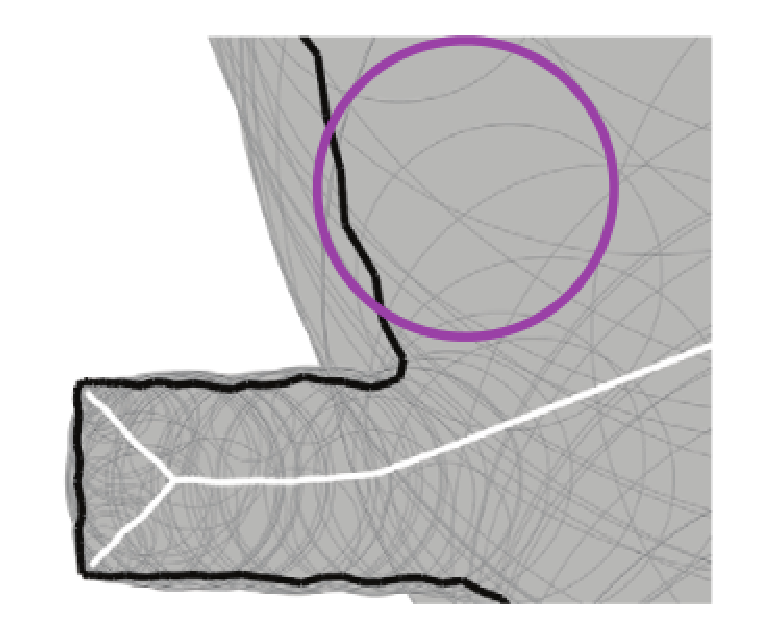
\epsfig{file = StableMedialAxis1.eps, width = 4.5cm}}
 \subfigure[Pruned]{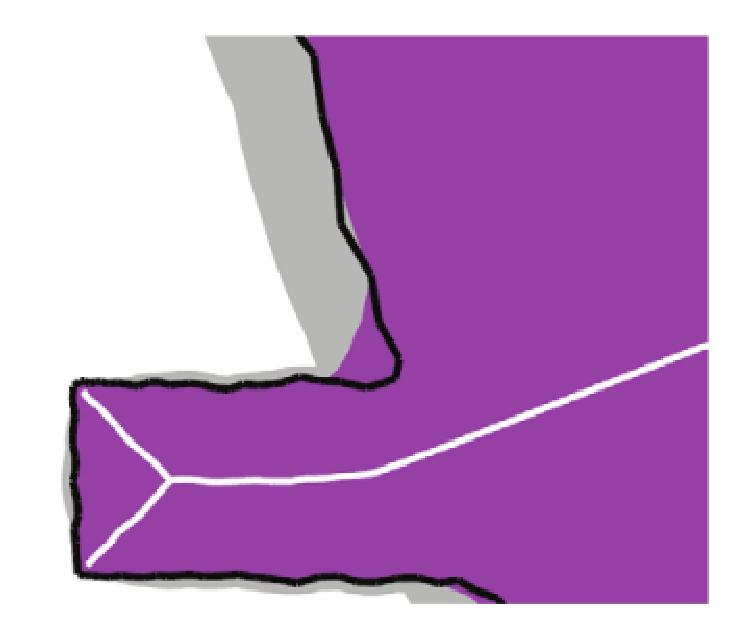
\epsfig{file = StableMedialAxis2.eps, width = 4.5cm}}
 \caption[MA Pruning.]{Image taken from \cite{miklos2010discrete}. Pruning the medial axis to detect important features.}
 \label{fig:stableAxis}  
\end{figure}

To get an insight of one technique to compute a stable MA, let us take the example in 
figure \ref{fig:stableAxis}. Figure \ref{fig:stableAxis}.a shows 
the MA in white and a medial inscribed disk in purple.
Figure \ref{fig:stableAxis}.b shows the same disc scaled by $\delta$. 
When all discs are scaled, large discs cover smaller nearby
discs. Covered discs belong to branches that can be trimed. 

Using this criterion, the branches can be pruned using a
scaling factor $\delta$, keeping only the larger discs 
that belong to the 'substance' of the object.

Figure \ref{fig:stableAxis}.c shows the simplified MA after
the shrinking of the discs by the same $\delta$. 
This procedure detects the least important branches on the MA, and
by pruning them, the amount of data to represent the same figure with out loosing 
much precision is significantly reduced. 

One important aspect left unanswered is if this type of representation 
is adequate to perform statistical analysis on a population of objects. 
One major difficulty will be to produce the correspondence of the branching structures.
Statistics on branching objects is a subject of ongoing research by \cite{wang2007object}, \cite{sorensen2011dissimilarity}, 
\cite{aydin2011visualizing}, 
which is still not applicable to medial geometry. 
To use medial representations for statistical analysis on shape, 
the construction of the MA must be done in a different manner: 
the MA should have a stable structure for the population of objects we wish to represent. 

If we take into consideration how the MA is built, we see that the procedure is a top-down approach, 
it starts on the boundary of the object and by using a certain criteria it gets to the MA. 
Another alternative is to operate the opposite way (down-top). 
We can find a down-top approach to build a MA in \cite{styner2001medial}.

In summary, Styner's method goes by computing an average MA
from a population of objects and then sampling the average using a regular grid of
points. The sampled grid of points is used as the new MA.
To compute the average MA, a PDM of
the branching structures is created 
by finely sampling their SPHARM representations.
The PDM allows PCA to compute the average and 
finally the grid of points or m-rep (definition given shortly) is sampled by 
minimizing a distance function over the points.
A series of tests are performed afterwards to assess
the quality of the MA by 
generating different instances of the population using 
the PCA coefficients. For each instance, the m-rep is refitted,
and an error measurement is estimated to evaluate 
how well it represents the whole population. 

\begin{figure} 
 \centering  
 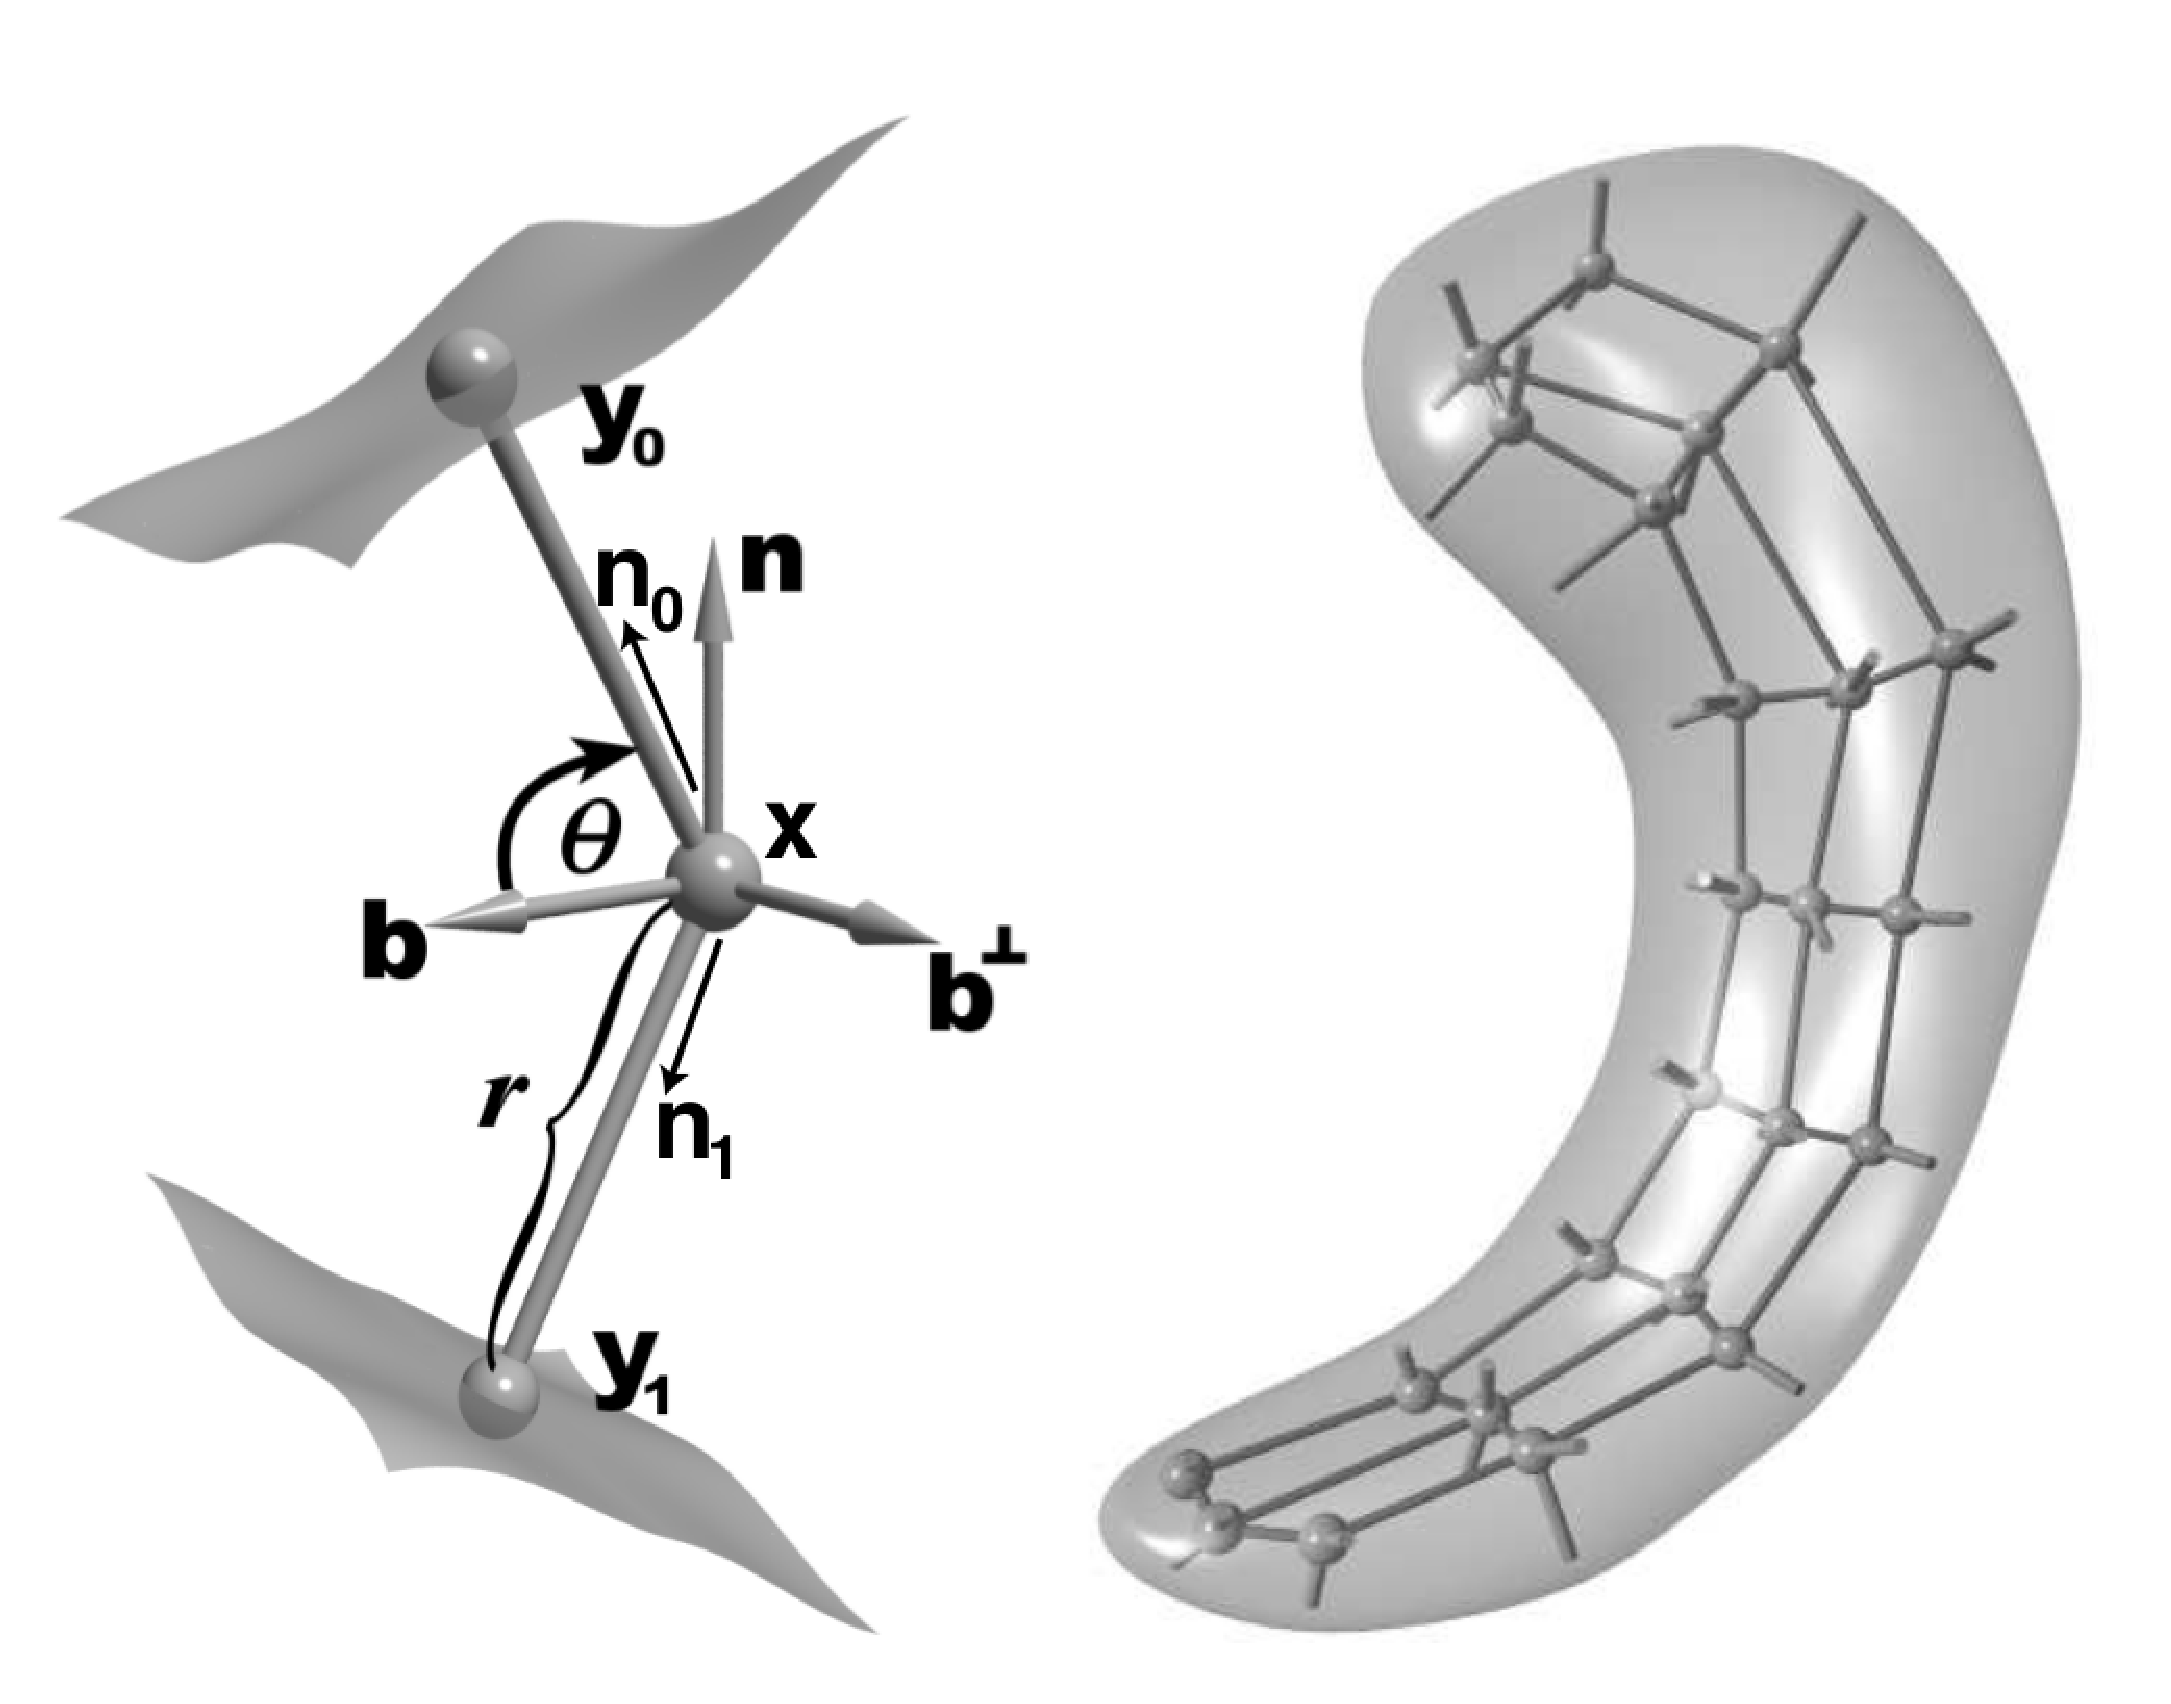
\epsfig{file = medialGeometry.eps, width = 8cm}
 \caption[Medial atom definition.]{Image taken from \cite{fletcher2004principal}. Medial atom definition (left) and a set of atoms representing a hippocampus (right).
          The atoms are arranged in a grid size $8*3$ and are able to produce the boundary of the hippocampus.}
 \label{fig:3DmedialGeometry}  
\end{figure}

M-reps are continuous objects that define the MA of an object as 
a set of connected manifolds \cite{pizer1999segmentation},  \cite{yushkevich2003continuous}, \cite{pizer2003deformable}.
Figure \ref{fig:3DmedialGeometry} shows the components of the medial geometry. 
The MS (medial sheet, equivalent to MA in 2D)
is parameterized by $MS(u, v)$ where $u$ and $v$ can take any value between 
$[0, 1] \in R$. 
The MS is a $C^2$ continuous set of medial atoms with a corresponding
implied boundary $y_{0}$ for top surface and $y_{1}$ for bottom surface. 

\begin{equation}
 MS(u, v) = \{x, r, n_0, n_1\}
 \label{equ:medialSheetAtom}
\end{equation}
Equation \ref{equ:medialSheetAtom} defines an atom for 
every $(u, v)$ on the MS, 
where $x$ is the position on the MS, $n_0$ and $n_1$
are the unit spoke directions, and $r$ is the 
length of both vectors. 

A different type of atom is found at the edges of the figure, named crest atoms.
Figure \ref{fig:crestAtom} shows how the top and bottom surfaces join 
at the crest to produce the closed boundary of the object. 

\begin{figure} 
 \centering  
 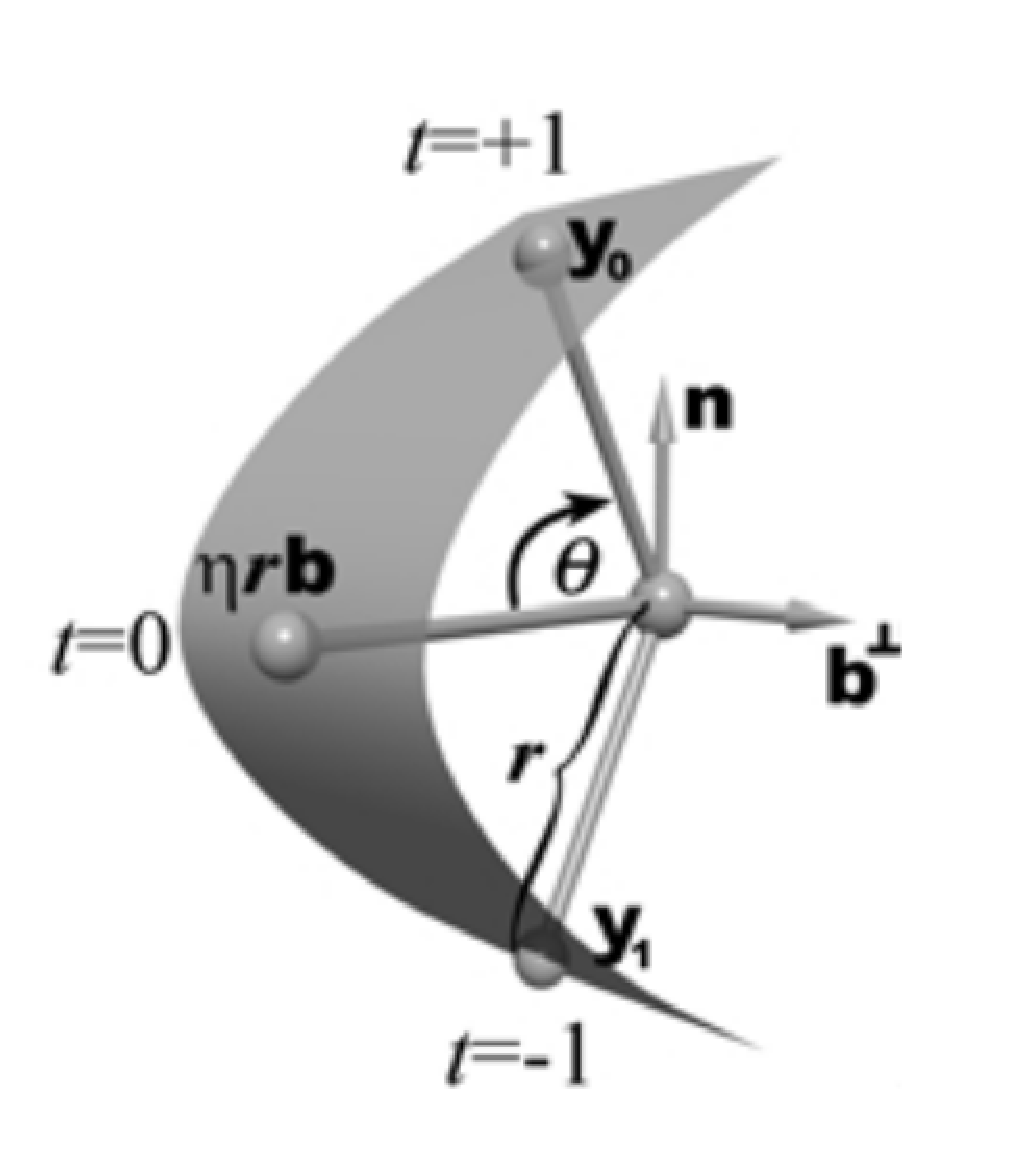
\epsfig{file = crestAtom.eps, width = 8cm}
 \caption[Top, bottom and crest surfaces.]{Image taken from \cite{pizer2003deformable}. Top and bottom surfaces of the m-rep join at the crest.}
 \label{fig:crestAtom}  
\end{figure}

To describe an m-rep in the computer, 
a discrete set of atoms is used.
From now on, the word m-rep relates to the discrete version of the object. 
M-reps use the interpolation mechanisms described in \cite{thall2004deformable}, 
which enables to reconstruct the object's surface.
The interpolation matches the surface 
to the normals described by the vectors $n_0$ and $n_1$.
Matching the normals produces a $C^2$ continuous surface everywhere. 
%From this surface Thall’s method allows the calculation of the interpolated medial atoms.

In summary, m-reps are efficient structures 
that describe in a multi-scale fashion the geometry
of an object, they can be used 
for medical image segmentation \cite{pizer2005method} and perform 
statistical analysis on shape variability \cite{fletcher2004principal}. 

The method used by m-reps to produce statistics is called PGA (principal geodesic analysis)
a generalization of PCA to manifold data, which will be described briefly in the 
following section.

\subsubsection{Principal geodesic analysis}

We have seen that m-reps can represent a population of 3D figures
by defining a stable MS and deforming it to best fit 
the various instances of the objects.
One of the many strengths of m-reps is to describe 
shape changes in terms of thickness, bending and widening 
among the already known variations (translation, rotation and scale).
In order to describe these variations 
standard techniques to compute statistics such as PCA do not apply, 
since m-reps are composed by elements of a non-Euclidean space.
In fact they belong to a Riemannian symmetric space.

If we recall the definition of a medial atom \ref{equ:medialSheetAtom},
we see that it is composed by $x \in R^3$, the center of the
inscribed sphere; $r \in R^+$, the local width defined as the
common spoke length; $n_0, n_1 \in S^2$, the two unit spoke
directions (here $S^2$ is the unit sphere in $R^3$).
The medial atom is then a point on the manifold
$M(1) = R^3 \times R^+ \times S^2 \times S^2$. 
Since an m-rep consists of $n$ medial atoms, 
a single figure may be considered as a point
on the manifold $M(n) = \Pi_{i=1}^n M(1)$ i.e., the direct product
of n copies of $M(1)$.

PGA (principal geodesic analysis) was developed as a generalization of PCA
for manifold data. 
The idea is to project the data onto lower-dimensional 
subspaces that best represent the variability of the data. 
Concepts from PCA such as mean, variance, subspace and projection 
had to be revisited in order to work properly with manifold data.
Details of PGA can be found in \cite{fletcher2004principal}.

PGA works well for data living on manifolds with spherical components, 
especially when the data is concentrated on a great circle path 
since the procedure fits the best great circle to describe these variations.
However, m-rep data frequently lives on small circles
as the mean computed with PGA is not optimal.
A more suitable statistical framework can be developed taking this into consideration. 

The following section describes quasi-medial representations or s-reps and
the statistical framework to compute shape variations called CPNS (composite 
principal nested spheres).


\subsection{Quasi-medial representations}
\label{sec:quasiMedial}

Quasi-medial representations or s-reps \cite{pizer_nested_2012} differ from m-reps on the strict medialness
constraint on every atom, i.e., the position of an atom is not necessarily the center 
of a maximally inscribed sphere. 
In s-reps, the atoms are rewarded for being ``as medial as possible'' but small 
deviations are tolerated, this means that the spokes can have different lengths;
this is done to improve the fit of an s-rep to a given object.

S-reps are continuous objects, defined as a locus of spoke vectors $(p, S)$ 
with tail at $p$ and tip at $p + S$, also parameterized by $(u, v)$ such that 
the skeletal sheet is defined as $SS = \{p(u, v) : \forall (u, v) \in [0, 1] \}$, the
spokes $SP = \{S(u, v) : \forall (u, v) \in [0, 1] \}$ and 
the boundary of the object is $BO = \{p(u, v) + S(u, v) : \forall (u, v) \in [0, 1] \}$.
The union of tails form the skeletal locus as a fully folded 
multi-sided sheet, i.e., the top side of the sheet is parameterized by $v \in [0, 0.5]$
and the bottom side by $v \in [0.5, 1]$.
Given this definition, every point inside the object can be reached by at least one spoke; 
special care in the corners of the object since they are reached by multiple spokes but allow the SS 
to fold and create the interior filling representation.

The lengths of the spokes are defined as $r(u, v) = |S(u, v)|$ and 
the directions of the spokes as $U(u, v) = S(u, v)/r(u, v)$. 
Figure \ref{fig:srepFigure}-a shows a slab figure parameterized
by $(u, v, \tau)$. $\tau \in [0, 1]$ is the portion of the spoke length from the SS to the boundary of the object.
The s-rep description can be used on tubular objects also. 
The tube figure is parameterized by $(u, \phi, \tau)$. Figure \ref{fig:srepFigure}-b shows the 
interior filling representation of a tubular object.

Section \ref{sec:internalCoordinates} extends the concept of interior filling objects and
the generation of $X2U$ (world coordinates to s-rep coordinates) and $U2X$ (s-rep coordinates to world coordinates) maps. 

\begin{figure} 
 \centering  
 \subfigure[Slab]{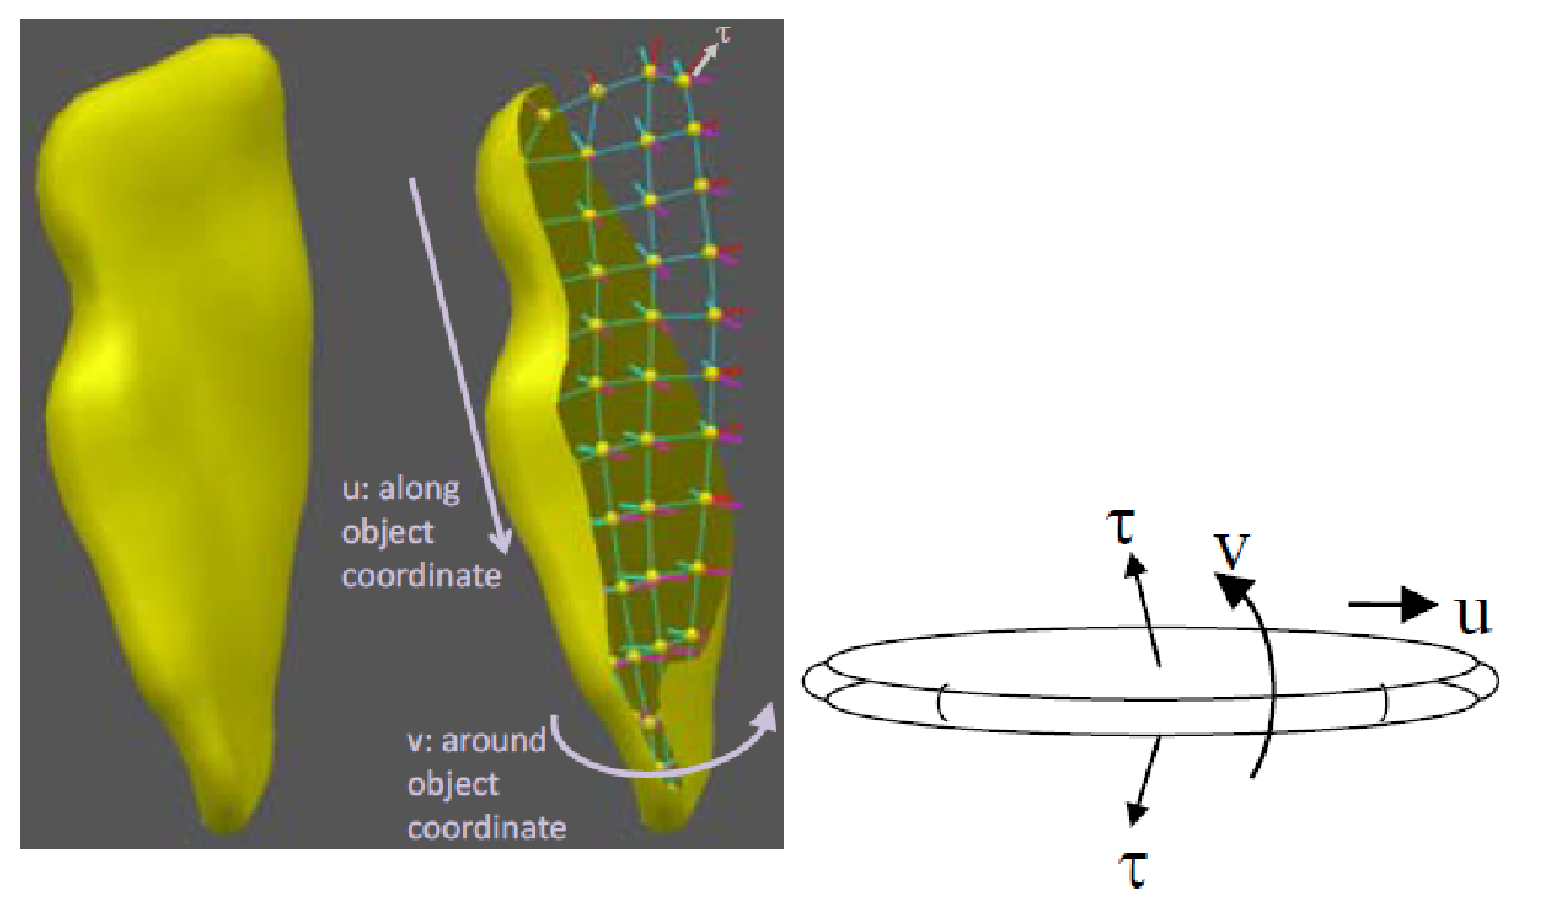
\epsfig{file = s-repSlab.eps, width = 16cm}}
 \subfigure[Quasi-tube]{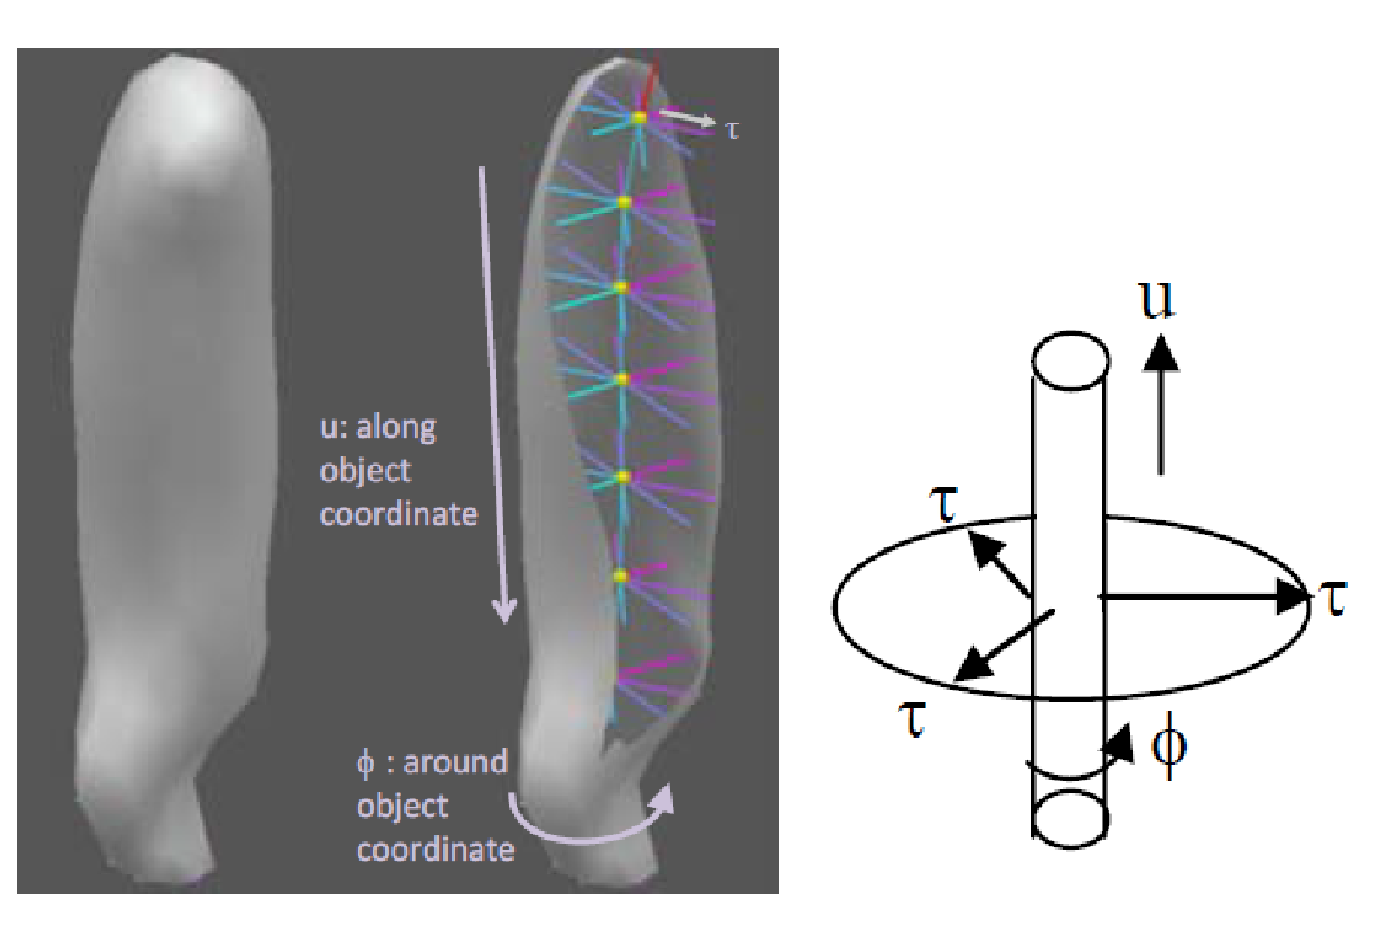
\epsfig{file = s-repTube.eps, width = 16cm}}
 \caption[Slab type s-rep.]{Image taken from \cite{pizer_nested_2012}. S-rep slab, interior filling object. Parameterized by $(u, v, \tau) \in [0, 1]$
          every point inside the object can be reached by only one spoke. 
          Similarly a tube figure is parameterized by $(u, \phi, \tau)$, $\phi$ is the rotation around the space curve that defines the MA.}
 \label{fig:srepFigure}  
\end{figure}

In a similar manner to m-reps, in the computer, s-reps are represented with a discrete set of atoms. 
From now on, s-rep is the discrete version of the object. 
S-reps use the interpolation mechanisms described in \cite{damon2003smoothness},
\cite{han2006interpolation}, \cite{damon2008swept} to produce a smooth skeletal locus and a smooth vector field of spokes that generates the 
boundary of the object.
For slab figures, represented as a $m \times n$ grid of atoms, 
the interpolation defines operators called $S_{rad}(u, v)$ and $S_E(u, v)$, 
applicable to non-fold medial points (top and bottom side of the sheet without the edges) and to the edge of the figure respectively.
The operators are defined as $2 \times 2$ matrices that can be computed for each spoke. They describe how the vector
$U(u, v)$ moves along and across the field of spokes. To interpolate a spoke at position $(u + \Delta u, v + \Delta v)$ 
the method uses the eigen-decomposition of the matrices. Damon shows that the object remains legal i.e., the spokes
do not cross each other,
if and only if for all $(u, v)$ the eigenvalues of $S_{rad}(u, v) < 1/r(u,v)$. 

The field of spokes can be retrieved by taking a small $\Delta$ step in the $(u, v)$ direction and interpolating  
the eigenvalues found from the eigen-decomposition of the matrix. 
The interpolation is done using the neighboring discrete spokes in the quad.

A quad is defined as
\begin{equation}
 Q_{i,j} = \{S(\frac{i}{n}, \frac{j}{m}), S(\frac{i+1}{n}, \frac{j}{m}), S(\frac{i+1}{n}, \frac{j+1}{m}), S(\frac{i}{n}, \frac{j+1}{m}) : i \in [1, n-1], j \in [1, m-1] \}]
 \label{equ:Quad}
\end{equation}
  
At each $(u + \Delta u, v + \Delta v)$ new eigenvalues 
are calculated that can be turned back into an $S_{rad}$ operator. Integrating $S_{rad}$
from $(u, v)$ at the corner to $(u + \Delta u, v + \Delta v)$ following a straight line, 
the full swing of the spoke can be computed. 

Besides object modeling using the interpolation mechanisms just described, 
the goal is to produce s-reps suitable for probabilistic analysis. 
Similarly to m-reps, the MS on an s-rep figure must remain 
stable through the population of objects.
S-reps go through a fitting process to produce the best possible
representation for each subject in the population. 
The procedure has mainly 3 stages to produce the fit. 
First, the s-rep is aligned to the image;
second, each atom is moved around separately to improve the fit; 
third, the spoke lengths are modified to further match the object's
boundary.
Further details are given in the following section.

\subsubsection{S-rep fitting}

The fitting process is done to produce the best 
geometric approximation of an object using 
a base s-rep, thus, stabilizing 
the MS through the population and giving the possibility to 
compute better statistics afterwards.
For the case of s-reps, instead of GPA, CPNS (Composite Principal Nested Spheres) is used.

The s-rep fitting is done on already segmented data, usually provided 
in the form of a binary image. The image is converted into 
a signed distance transform \cite{saboo2011aa}, with negative values 
in the interior, 0 at the boundary and positive outside of the object. 
After the conversion, 
the fitting starts by aligning the s-rep to the data
via matching of moments of boundary positions (zero level on the distance transform) or using 
landmarks provided by the user.

In the second stage or atom stage, each atom in the s-rep is optimized
by measuring how well each of the spokes fits into the distance image $D(x)$ while maintaining 
the regularity of the grid. In this stage, the only variable affected is the position and orientation of the atom. 

In the third stage or spoke stage, each spoke is optimized to produce the best match to the boundary of the object
while fixing the tail and changing the angle and length of the spokes.

The following penalties are used to produce the fit:
\begin{enumerate}
 \item Regularity of the quads (see Equation \ref{equ:Quad} for quad definition). 
 \item Deviation from medialness using the spokes located at opposite sides of the MS $|r(u, v) - r(u, 1 - v)|$. 
 \item Deviation of spoke directions from boundary normals $cos^{-1}(\hat{\nabla D(x)} \cdot U(u, v))$ where $x = p(u,v) + S(u, v)$.
 %\item Deviation from MS normals. The MS normal is calculated as $U(u,v) - U(u,1 - v)$.
 \item Deviation at the crest from the angle between $w_2$ and $U(u, v) \times U(u, 1 - v)$, where $w_2$ is orthogonal to the principal curvature direction.
 \item Illegality of spoke crossings, i.e.,  $S_{rad}(u, v) > 1/r(u,v)$ 
\end{enumerate}

Once the optimization described above is done for every object in the population, 
correspondence among the cases must be achieved prior to computing 
statistics using CPNS; this can be done by using the SS that is composed by 
a set of points $\{p_i\}$ as a PDM. The PDM can be centered at the origin and 
then scaled by making the 
sum of the squared distances of the points to the origin equal to 1.
The scaling factor of the PDM will be named $\lambda$.
After the alignment, in order to produce shape statistics, let us analyze the 
abstract space where an s-rep lives.

\subsubsection{S-rep abstract space and composite analysis}

An s-rep lives in $R^{n+1} \times S^{3n - 4} \times (S^2)^n$.
To explain this abstract space, let us
define one s-rep composed by $n$ spokes $s_{rep} = \{(p_i, r_i, U_i) | i = 1,2, ...,n\}$.
This corresponds to the Cartesian product of $n + 2$ manifolds, 
one of which is Euclidean and the rest are spheres.
The Euclidean manifold $R^{n+1}$ corresponds to $n$ log $r_i$ values plus 
the scaling factor of the PDM (log $\lambda$).
The spherical manifolds are the $S^{3n - 4}$ corresponding to the PDM
and the $(S^2)^n$ are for the $n$ spoke directions.

In order to study a population of s-reps and knowing that 
they are composed by elements on different manifolds, 
each one of them is analyzed separately at first.

PNS (principal nested spheres) \cite{jung_analysis_2012} allows 
estimating the principal modes for each non-Euclidean component
and produces Euclidean scores (see Appendix \ref{sec:apendixCPNS}).
All of the scores are composed on a matrix 
that contains Euclidean data only, thus, 
making possible to do further analysis using PCA. 
The composite matrix $Z_{comp}$ is shown in Equation \ref{equ:compositeMatrix}, where $N$ is the number
of s-reps and * means that the mean has been subtracted from the variable. 

\begin{equation}
\begin{array}{ccc}
         \begin{array}{c}         
          \text{Sphere 0:} \\
          \text{Scaled medial points} \\
           \\
           \\
          \text{Spheres 1 - n:}\\          
          \text{Spoke directions} \\
          \\
          \text{Euclidean variables:}\\
          \text{Scaling}\\
          \\
          \\
          \text{Spoke lengths} \\          
          \\
         \end{array} 
 &
    \left [ \begin{array}{ccc}
          z^t_{1,1} & \hdots & z^t_{1,N} \\
          \vdots    & \ddots & \vdots    \\
          z^t_{N-1,1} & \hdots & z^t_{N-1,N}\\
          \\
          z^{S_1}_{1,1} & \hdots & z^{S_1}_{1,N}\\          
          \vdots    & \ddots & \vdots    \\
          z^{S_n}_{n,1} & \hdots & z^{S_n}_{n,N}\\          
          \\
          \text{log}^*_{\lambda_1} & \hdots & \text{log}^*_{\lambda_N} \\
          \\
          \text{log}^*_{r_{1,1}} & \hdots & \text{log}^*_{r_{n,N}} \\
          \vdots    & \ddots & \vdots    \\
          \text{log}^*_{r_{n,1}} & \hdots & \text{log}^*_{r_{n,N}} \\
         \end{array} \right ]
 &
    \left [ \begin{array}{c}
          \bar \lambda \\          
          \vdots \\
          \bar \lambda \\
          \\
          \bar r_1 \\          
          \vdots \\          
          \bar r_n \\
          \\
          \bar \lambda \\
          \\
          \bar r_1 \\
          \vdots \\
          \bar r_n \\
         \end{array} \right ]
\\
& \longleftarrow \text{Cases} \longrightarrow & \text{Scaling}
\end{array}
\label{equ:compositeMatrix}
\end{equation}

CPNS produces a set of eigenmodes that can be used to approximate 
any of the shapes in the population (see Appendix \ref{sec:apendixPCA}).
This results in a vector that lives in Euclidean space equivalent to the $Z_{comp}$ matrix.
Using this vector, each of the Euclidean components are ready to be mapped back to 
their corresponding spheres by adding the mean value computed at the PNS analysis. 

We have seen that it is possible to compute robust statistics for 3D shape objects using 
medial representations. The following section explains the implementation based 
on the concepts seen for medial representations. 

\section{Object modeling using s-reps }
\label{sec:s-repImplementation}

The s-rep implementation done for this dissertation defines
the interpolation mechanisms similar to \cite{han2006interpolation}.

\subsection{MS interpolation}

The interpolation is done with cubic Hermite splines.
To produce the interpolation, the partial derivatives for every atom on the SS, 
and the normal must be defined.

Let $s_{rep} = \{(p_i, S_i) : i \in N\}$ and $N = m \times n$, 
represent a discrete grid of atoms.
The interpolation is done using the four control points from each quad in the grid. 

%A quad is defined as 
%$Q_{i,j} = \{S(i/n, j/m), S((i+1)/n, j/m), S((i+1)/n, (j+1)/n), S(i/n, (j+1)/m) : i \in [1, n], j \in [1, m] \}]$)),
Equations \ref{equ:pDerivativeU} and \ref{equ:pDerivativeV} shows how to compute the partial derivative for a given atom 
in the $u$ and $v$ direction on the SS. $\Delta u = 1/m$ and $\Delta v = 1/n$ 
correspond to a step lenght. $u + \Delta u$ moves along the $u$ direction onto 
the next atom on the discrete grid, and similarly for the $v$ direction.

\begin{equation}
 \partial p(u, v)_u = \left \{ \begin{array}{ll}
                      p(u + \Delta u, v) - p(u , v) & u = 0\\
                      \big (p(u + \Delta u, v) - p(u - \Delta u, v)\big )/2 & 0 < u < 1 \\
                      p(u, v) - p(u - \Delta u, v) & u = 1
                     \end{array} \right .
\label{equ:pDerivativeU}
\end{equation}

\begin{equation}
 \partial p(u, v)_v = \left \{ \begin{array}{ll}
                      p(u, v + \Delta v) - p(u, v) & v = 0\\
                      \big (p(u, v + \Delta v) - p(u, v - \Delta v) \big ) /2 & 0 < v < 1 \\
                      p(u, v) - p(u, v - \Delta v) & v = 1
                     \end{array} \right .
\label{equ:pDerivativeV}
\end{equation}

Equation \ref{equ:sheetNormal} gives an approximation to the normal of an atom to the SS. 
The normal is computed from opposite spokes with tail at equal position on the SS. 
More precisely, $N$ is normal to the SS if the two spokes are exactly boundary normals 
and have the same lenght. 

\begin{equation}
  \begin{array}{cc}
   N(u, v) \approx \frac{S(u, v) - S(u, 1 - v)}{||S(u, v) - S(u, 1 - v)||}  & u  \in [0, 1], v \in [0, 0.5] \\
  \end{array}
\label{equ:sheetNormal}
\end{equation}

\begin{figure} 
 \centering  
 \subfigure[Level 0]{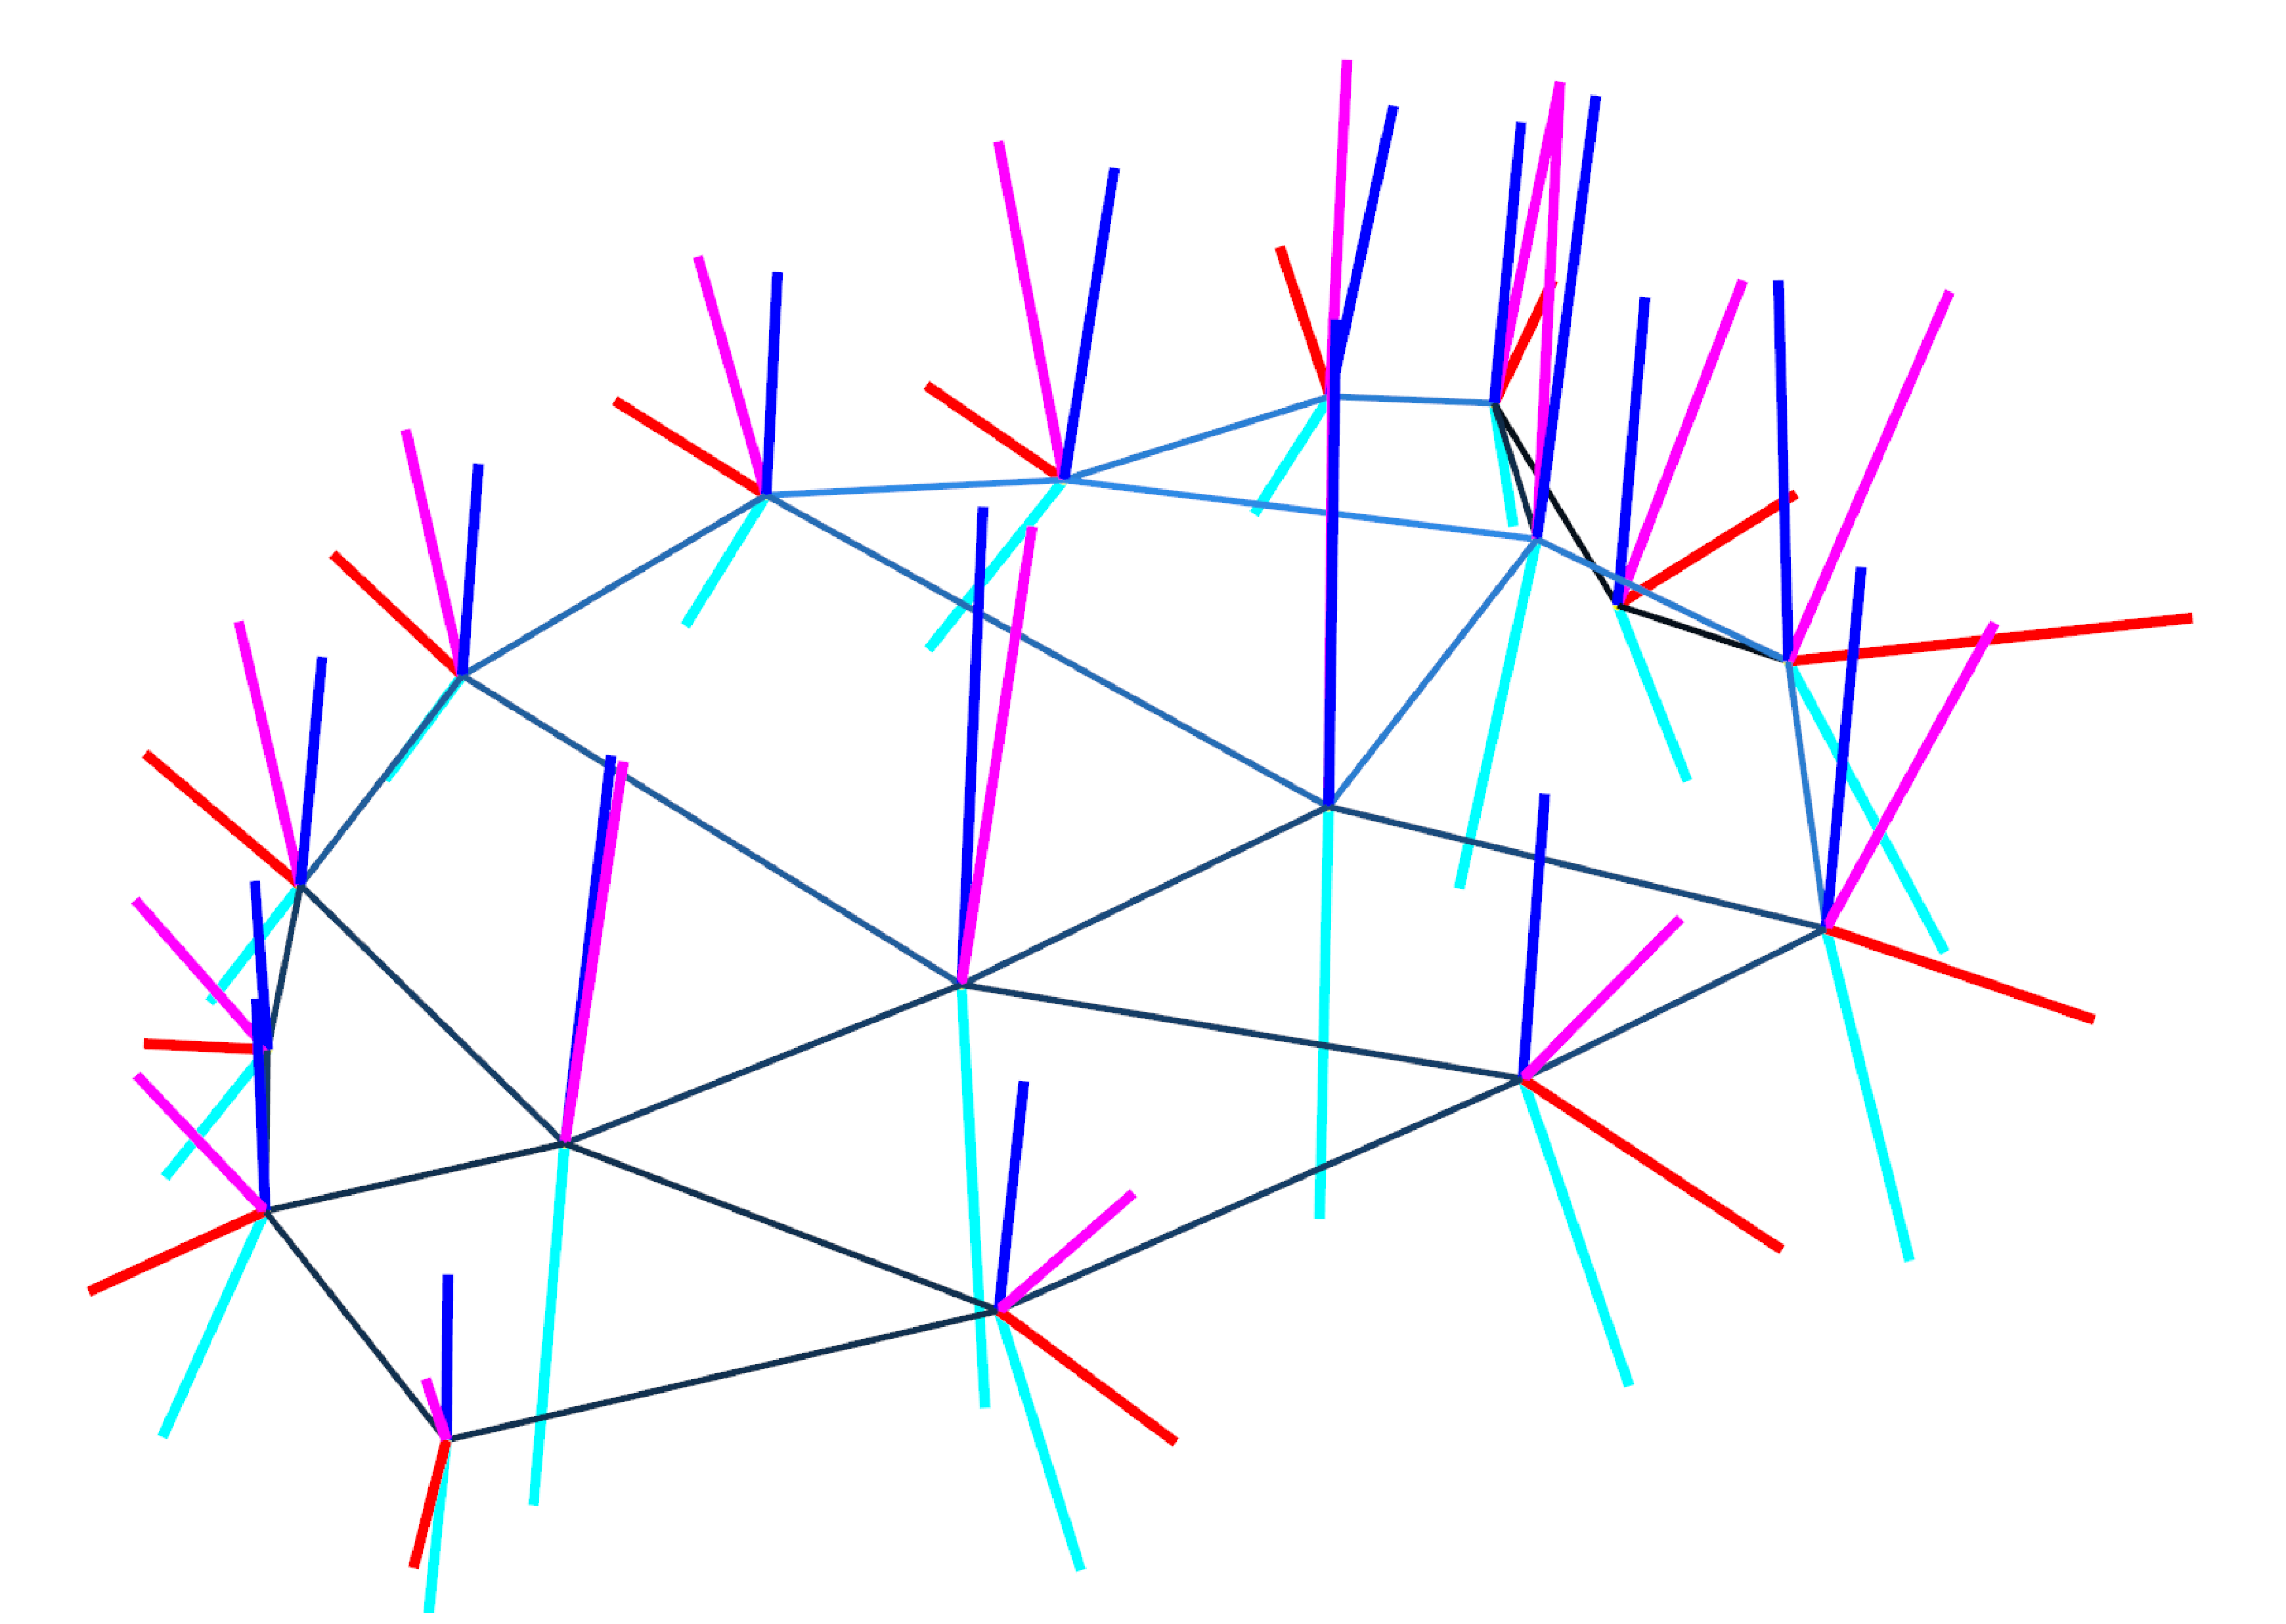
\epsfig{file = interpolationMedialSheet0.eps, width = 7cm}}
 \subfigure[Level 3]{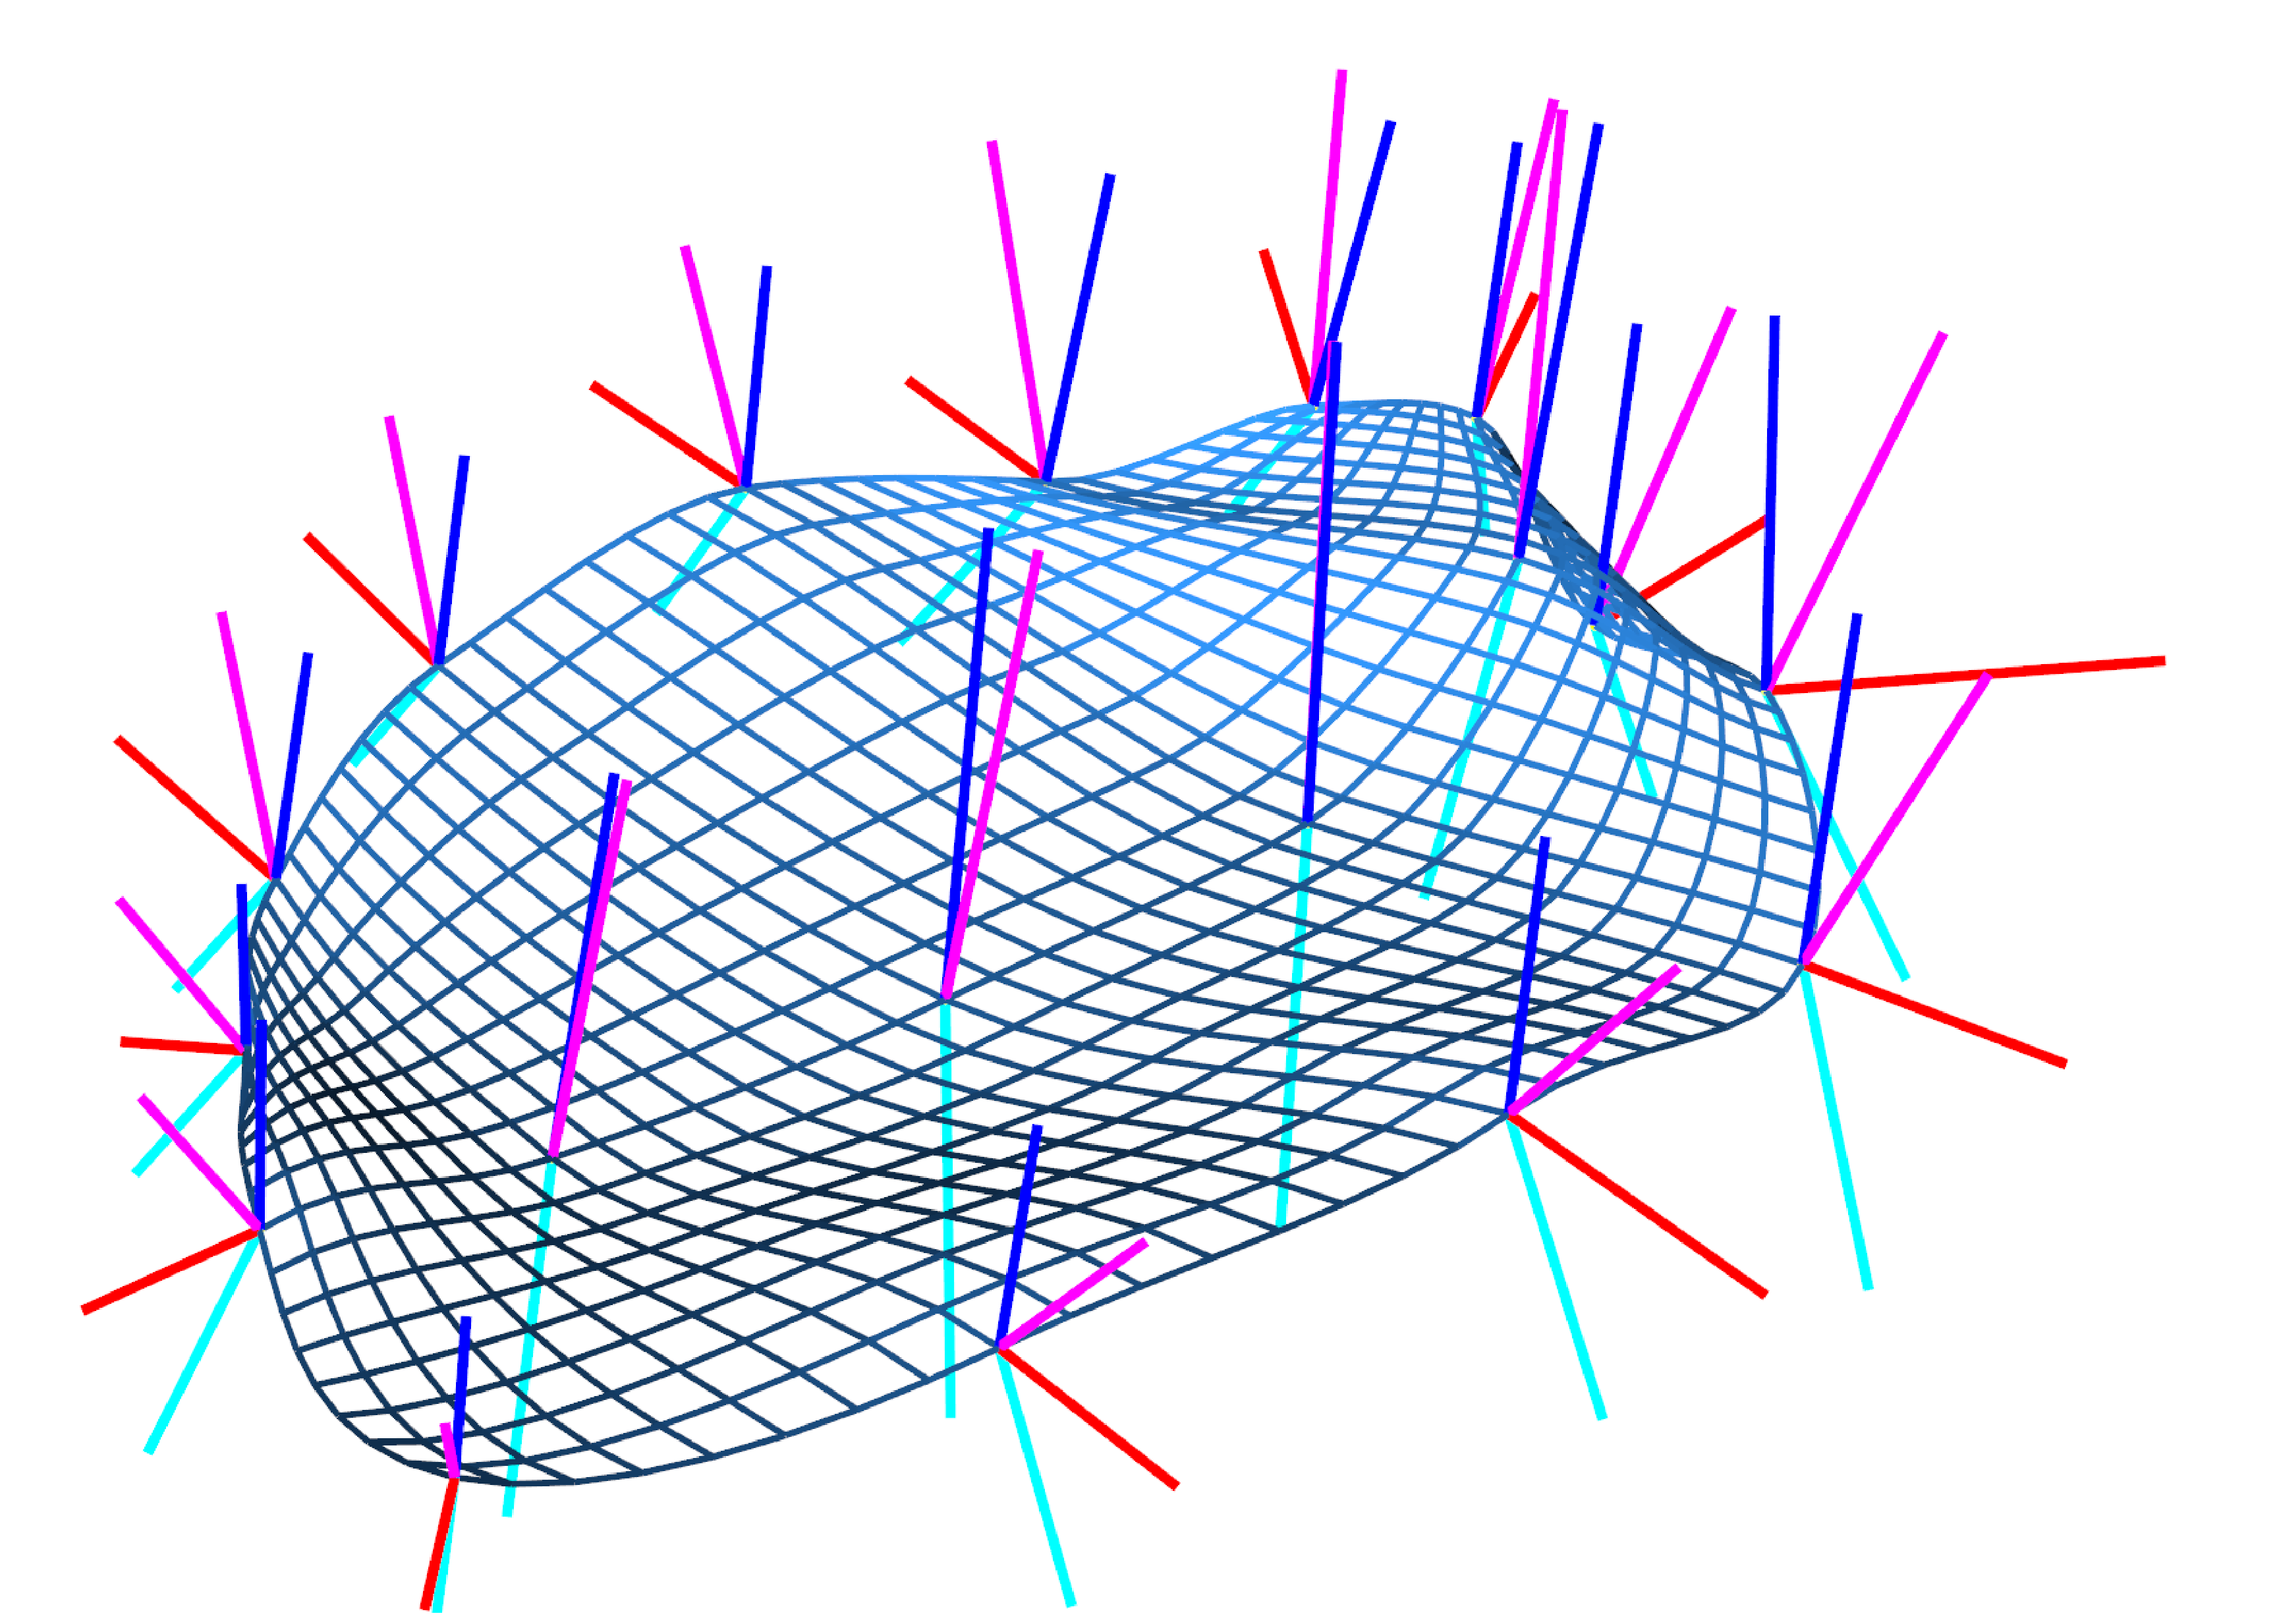
\epsfig{file = interpolationMedialSheet3, width =7cm}}
 \caption[Slab's MS interpolation.]{MS interpolation for a slab type s-rep. The top spoke is shown in magenta, the bottom spoke in cyan, the crest spoke in red,
          the MS is shown in light blue and the normal to the sheet is shown in blue.}
 \label{fig:interpolationMedialSheet}  
\end{figure}

\begin{equation}
 H_{control} = \left [ \begin{array}{cccc}
                    p_{11} & p_{12} 			& \partial p_{{11}_v}^T & \partial p_{{12}_v}^T \\
                    p_{21} & p_{22}			& \partial p_{{21}_v}^T & \partial p_{{22}_v}^T \\
                    \partial p_{{11}_u}^T & \partial p_{{12}_u}^T	& h_{0} & h_{0} \\
                    \partial p_{{21}_u}^T & \partial p_{{22}_u}^T	& h_{0} & h_{0} \\
                    
                   \end{array} \right ]
  \label{equ:hermiteControl}
\end{equation}

To interpolate the SS, a Hermite matrix patch is defined in equation \ref{equ:hermiteControl},
where $\partial p(u,v)^T = \partial p(u,v) - (\partial p(u,v) \cdot N(u, v))N(u,v)$ is the projection of the discrete derivatives in directions $u$ or $v$ onto the tangent planes
that are determined by the normals $N(u,v)$, so the MS interpolation depends on the normals and the discrete derivatives; $h_{0}$ is a vector filled with $0$. 

\begin{equation}
 \begin{array}{l}
  H_1(s)= 2s^3 - 3s^2 + 1\\
  H_2(s)= -2s^3 + 3s^2\\
  H_3(s)= s^3 - 2s^2 + s\\
  H_4(s)= s^3 - s^2\\
 \end{array}
\label{equ:weightFunctions}
\end{equation}

\begin{equation}
 p(u, v) = \left [ \begin{array}{cccc} H_1(\hat u) & H_2(\hat u) & H_3(\hat u) & H_4(\hat u) \end{array} \right ]
                H_{control}
           \left [ \begin{array}{c} H_1(\hat v) \\
				     H_2(\hat v) \\ 
				     H_3(\hat v) \\ 
				     H_4(\hat v) 
		    \end{array} \right ]
\label{equ:interpolatedPoint}
\end{equation}

The interpolated position for any atom on the SS is shown in equation \ref{equ:interpolatedPoint}, 
using a Hermite matrix control patch and the weight functions defined in \ref{equ:weightFunctions}.
$\hat u = (u - floor(u))/\Delta u$, where $floor(u)$ returns the $u$ coordinate of the atom at $p_{11}$,
similarly for $\hat v$, notice that every patch is interpolated by varying $(\hat u, \hat v): 0 \rightarrow 1$.
Figure \ref{fig:interpolationMedialSheet} shows the interpolation of the MS at different levels for the same figure.

In a similar manner, the spoke interpolation can be done using Hermite basis functions. Instead of using the control points
$p(u, v)$, the spokes $S(u, v)$ are used. Accordingly, the discrete derivatives are computed for each spoke, the difference
in this case is that no projection is done using the normals to the SS; the spoke interpolation only depends on the discrete derivatives. 


\begin{figure} 
 \centering  
 \subfigure[Interpolated spokes]{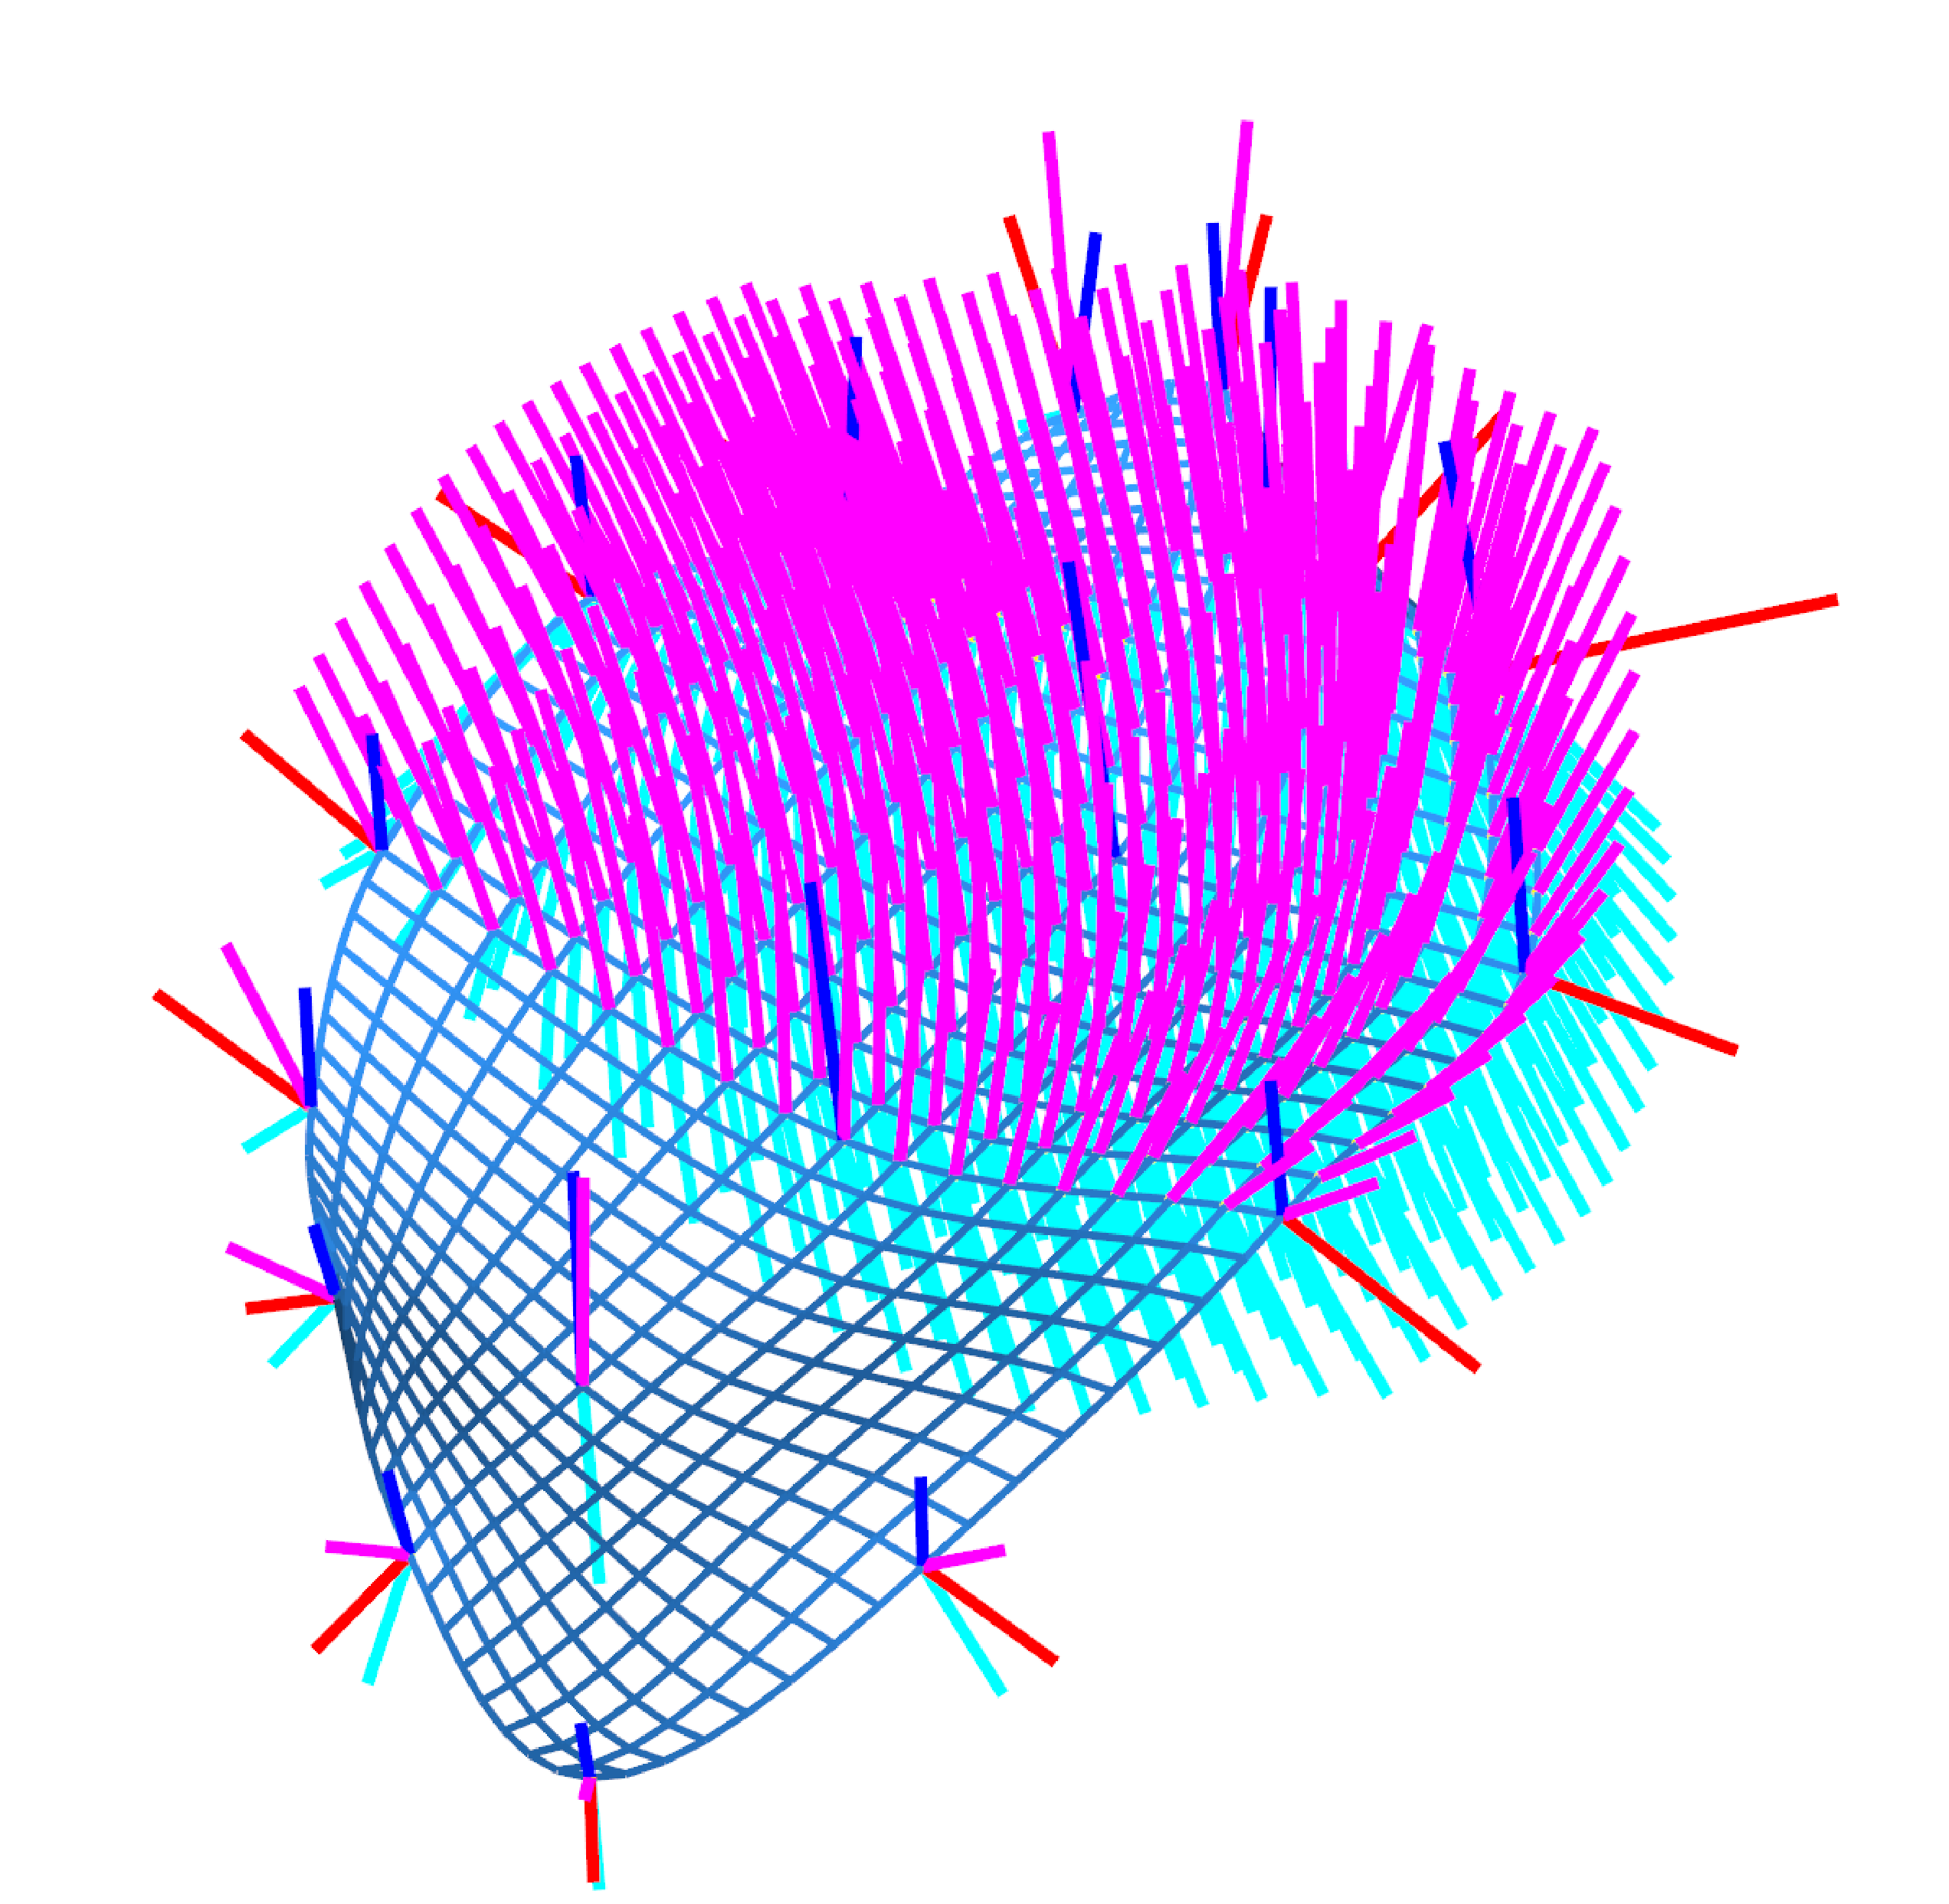
\epsfig{file = interpolationSpokes.eps, width = 7cm} }
 \subfigure[Union of spoke tips]{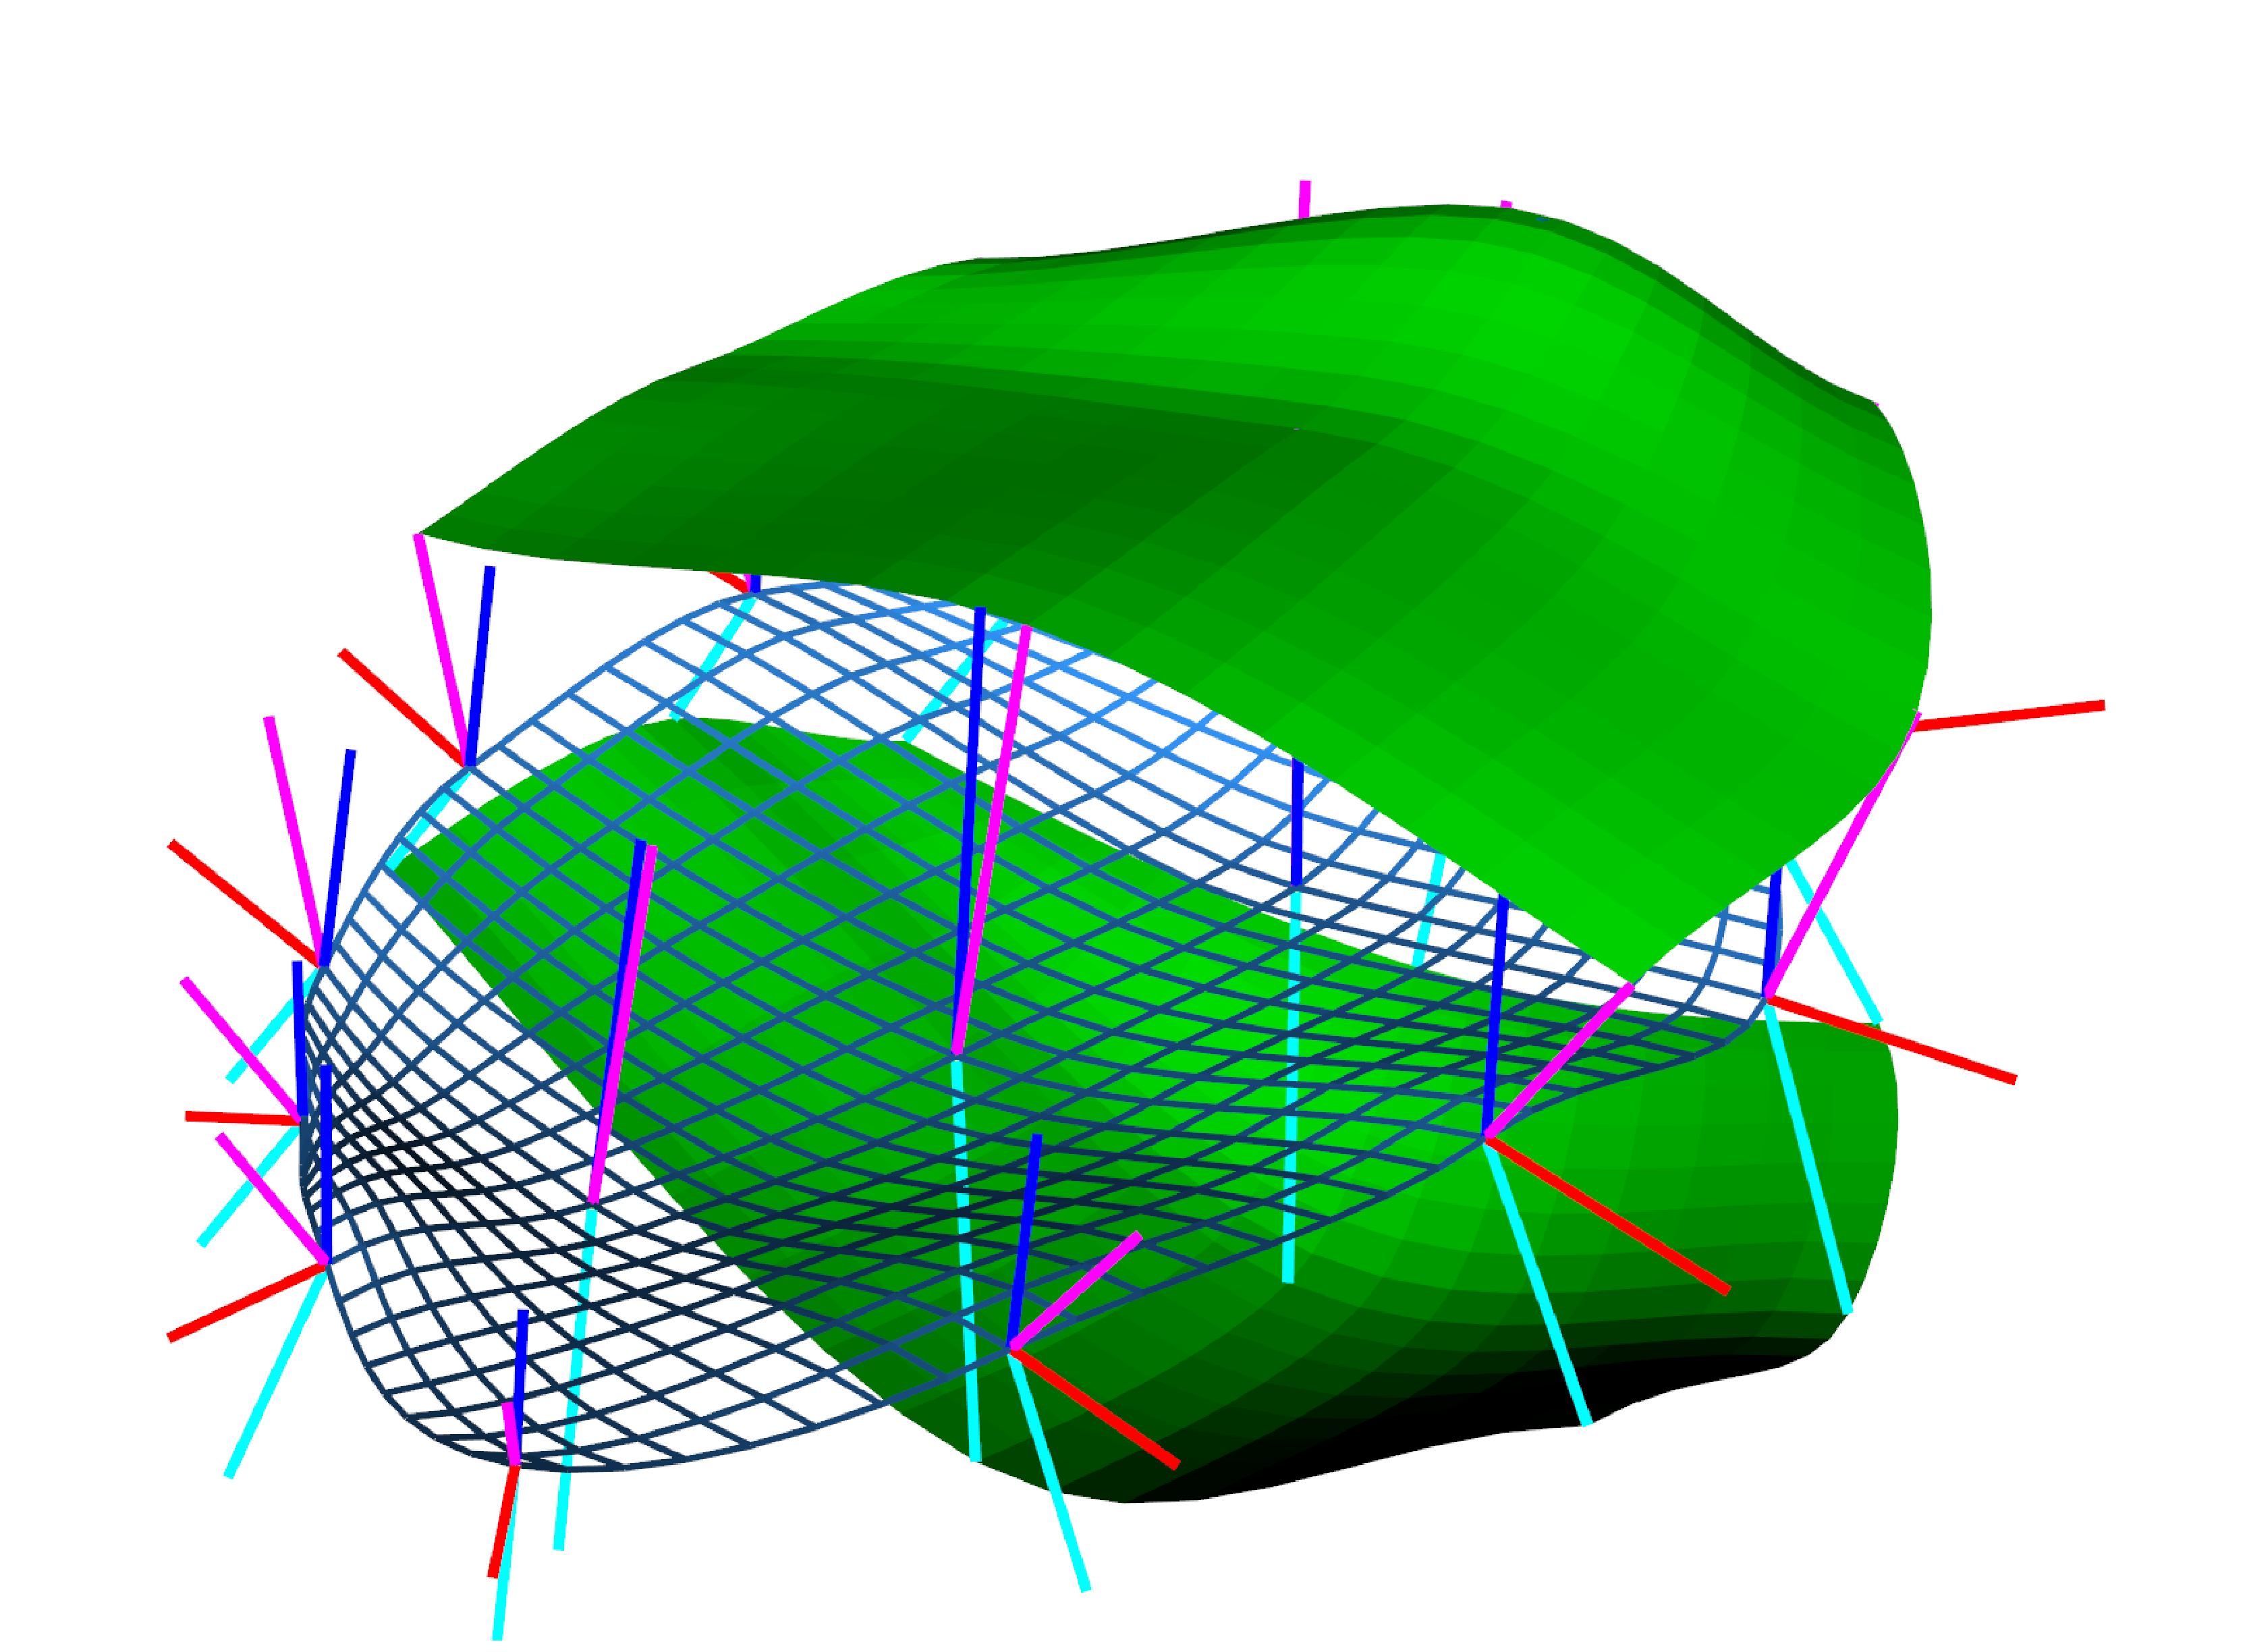
\epsfig{file = interpolationSurface3.eps, width = 7cm}}
 \caption[Top and bottom surface interpolation.]{Top and bottom surfaces interpolated for a given atom. The surfaces are generated from the spoke interpolation.}
 \label{fig:GeneratedSurfaceSpokeInterpolation}  
\end{figure}

The top and bottom surface can be generated using the mechanisms described above. 
Figure \ref{fig:GeneratedSurfaceSpokeInterpolation} shows the implied surface generated by the union of 
interpolated spoke tips.
As mentioned before, both surfaces meet at the crest of the object, 
Section \ref{sec:crestInterpolation} explains how to perform the crest interpolation which 
can also be used to interpolate tubular figures.

\subsection{Crest interpolation}
\label{sec:crestInterpolation}

For the crest interpolation, we wish to fit a surface that 
does not collapse towards the interior of the object. In other words, 
its cross-section should be convex
in the principal direction and preserve $C^2$ continuity. Another property of the surface is that the directional 
derivatives computed for every spoke should be matched in order to produce a smooth surface
to the Hermite based interpolation previously explained.

The crest interpolation method is explained by showing how to interpolate the lenghts $r$ of a spoke
that sweeps according to an angle $\theta$.
The function $r(\theta)$ returns the lenght at a given angle.
In a similar way, we wish to interpolate the cross-section in the crest, where theta 
runs between the terminus of the top or bottom spoke to the crest spoke. 

The same problem can be extended to 3 dimensions where the interpolation produces a space curve.
In order to produce an interpolated surface the interpolation of the cross-section 
sweeps along the skeletal sheet.

\begin{equation} 
 \frac{\partial^2 r(\theta)}{\partial \theta} = q_0  +  q_1  \theta + q_2  \theta^2  
 \label{equ:curvature}
\end{equation}

The first step is to define a quadratic function of the curvature, as shown in Equation
\ref{equ:curvature}, we would like to enforce convexity in the interpolated curve.
By integrating this equation twice, we find the function that gives us the length for $\theta \in [0, \theta_{max}]$.

\begin{eqnarray} 
  \frac{\partial r(\theta)}{\partial \theta} &=& \int_0^{\theta_{max}} \frac{\partial^2 r(\theta)}{\partial \theta} \partial \theta \\
  \frac{\partial r(\theta)}{\partial \theta} &=& \frac{\partial r_0}{\partial \theta} + q_0  \theta + \frac{1}{2}  q_1  \theta^2 + \frac{1}{3}  q_2  \theta^3  \\
  r(\theta) &=& \int_0^{\theta_{max}} \frac{\partial r(\theta)}{\partial \theta} \partial \theta \\
  r(\theta) &=& r_0 + \frac{\partial r_0}{\partial \theta}  \theta + \frac{1}{2}  q_0  \theta^2 + \frac{1}{6}  q_1  \theta^3 + \frac{1}{12}  q_2  \theta^4  
\end{eqnarray}

We start by solving for coefficients $q_1$ and $q_2$,
using the system of equations $r(\theta)$, $\partial r(\theta)/\partial \theta$ and $\partial^2 r(\theta)/\partial \theta$, 
as shown in equation \ref{equ:solveQ1}.

\begin{eqnarray} 
q_2 &=& \frac{6}{\theta_{max}^4} (2 \partial r_{end} \theta_{max} + q_0 \theta_{max}^2 - 6 r_{end} + 6 r_0 + 4 \partial r_0 \theta_{max}) \\
q_1 &=& \frac{-6}{\theta_{max}^3} (-\partial r_{end} + r_0 + \partial r_0 \theta_{max} +  \frac{q_0}{2} \theta_{max} + \frac{q_2}{12} \theta_{max}^4)
\label{equ:solveQ1}
\end{eqnarray} 

There exists a solution to the problem for every $q_0$ but
the optimal solution is found when $q_0$ minimizes the average 2nd derivative
of $r$ as shown in Equation \ref{equ:minimizeCurvature}.

\begin{equation}
 \partial r_{end} =  -1 \partial r_{end} = 0 \partial r_{end} = 1 r_0 \theta \partial r_0
\end{equation}


\begin{equation}  
  \hat q_0 = \operatorname*{arg\,min}_{q_0} \sum_{\theta = 0}^{\theta_{max}} \frac{\partial^2 r(\theta)}{\partial \theta}
  \label{equ:minimizeCurvature}
\end{equation}

Notice that the parameters $r_0$, $r_{end}$, $\partial r_0$ and $\partial r_{end}$ correspond to 
initial and final lengths, and rates of the change at $r_0$ and $r_{end}$ respectively.

\begin{figure} 
 \centering  
 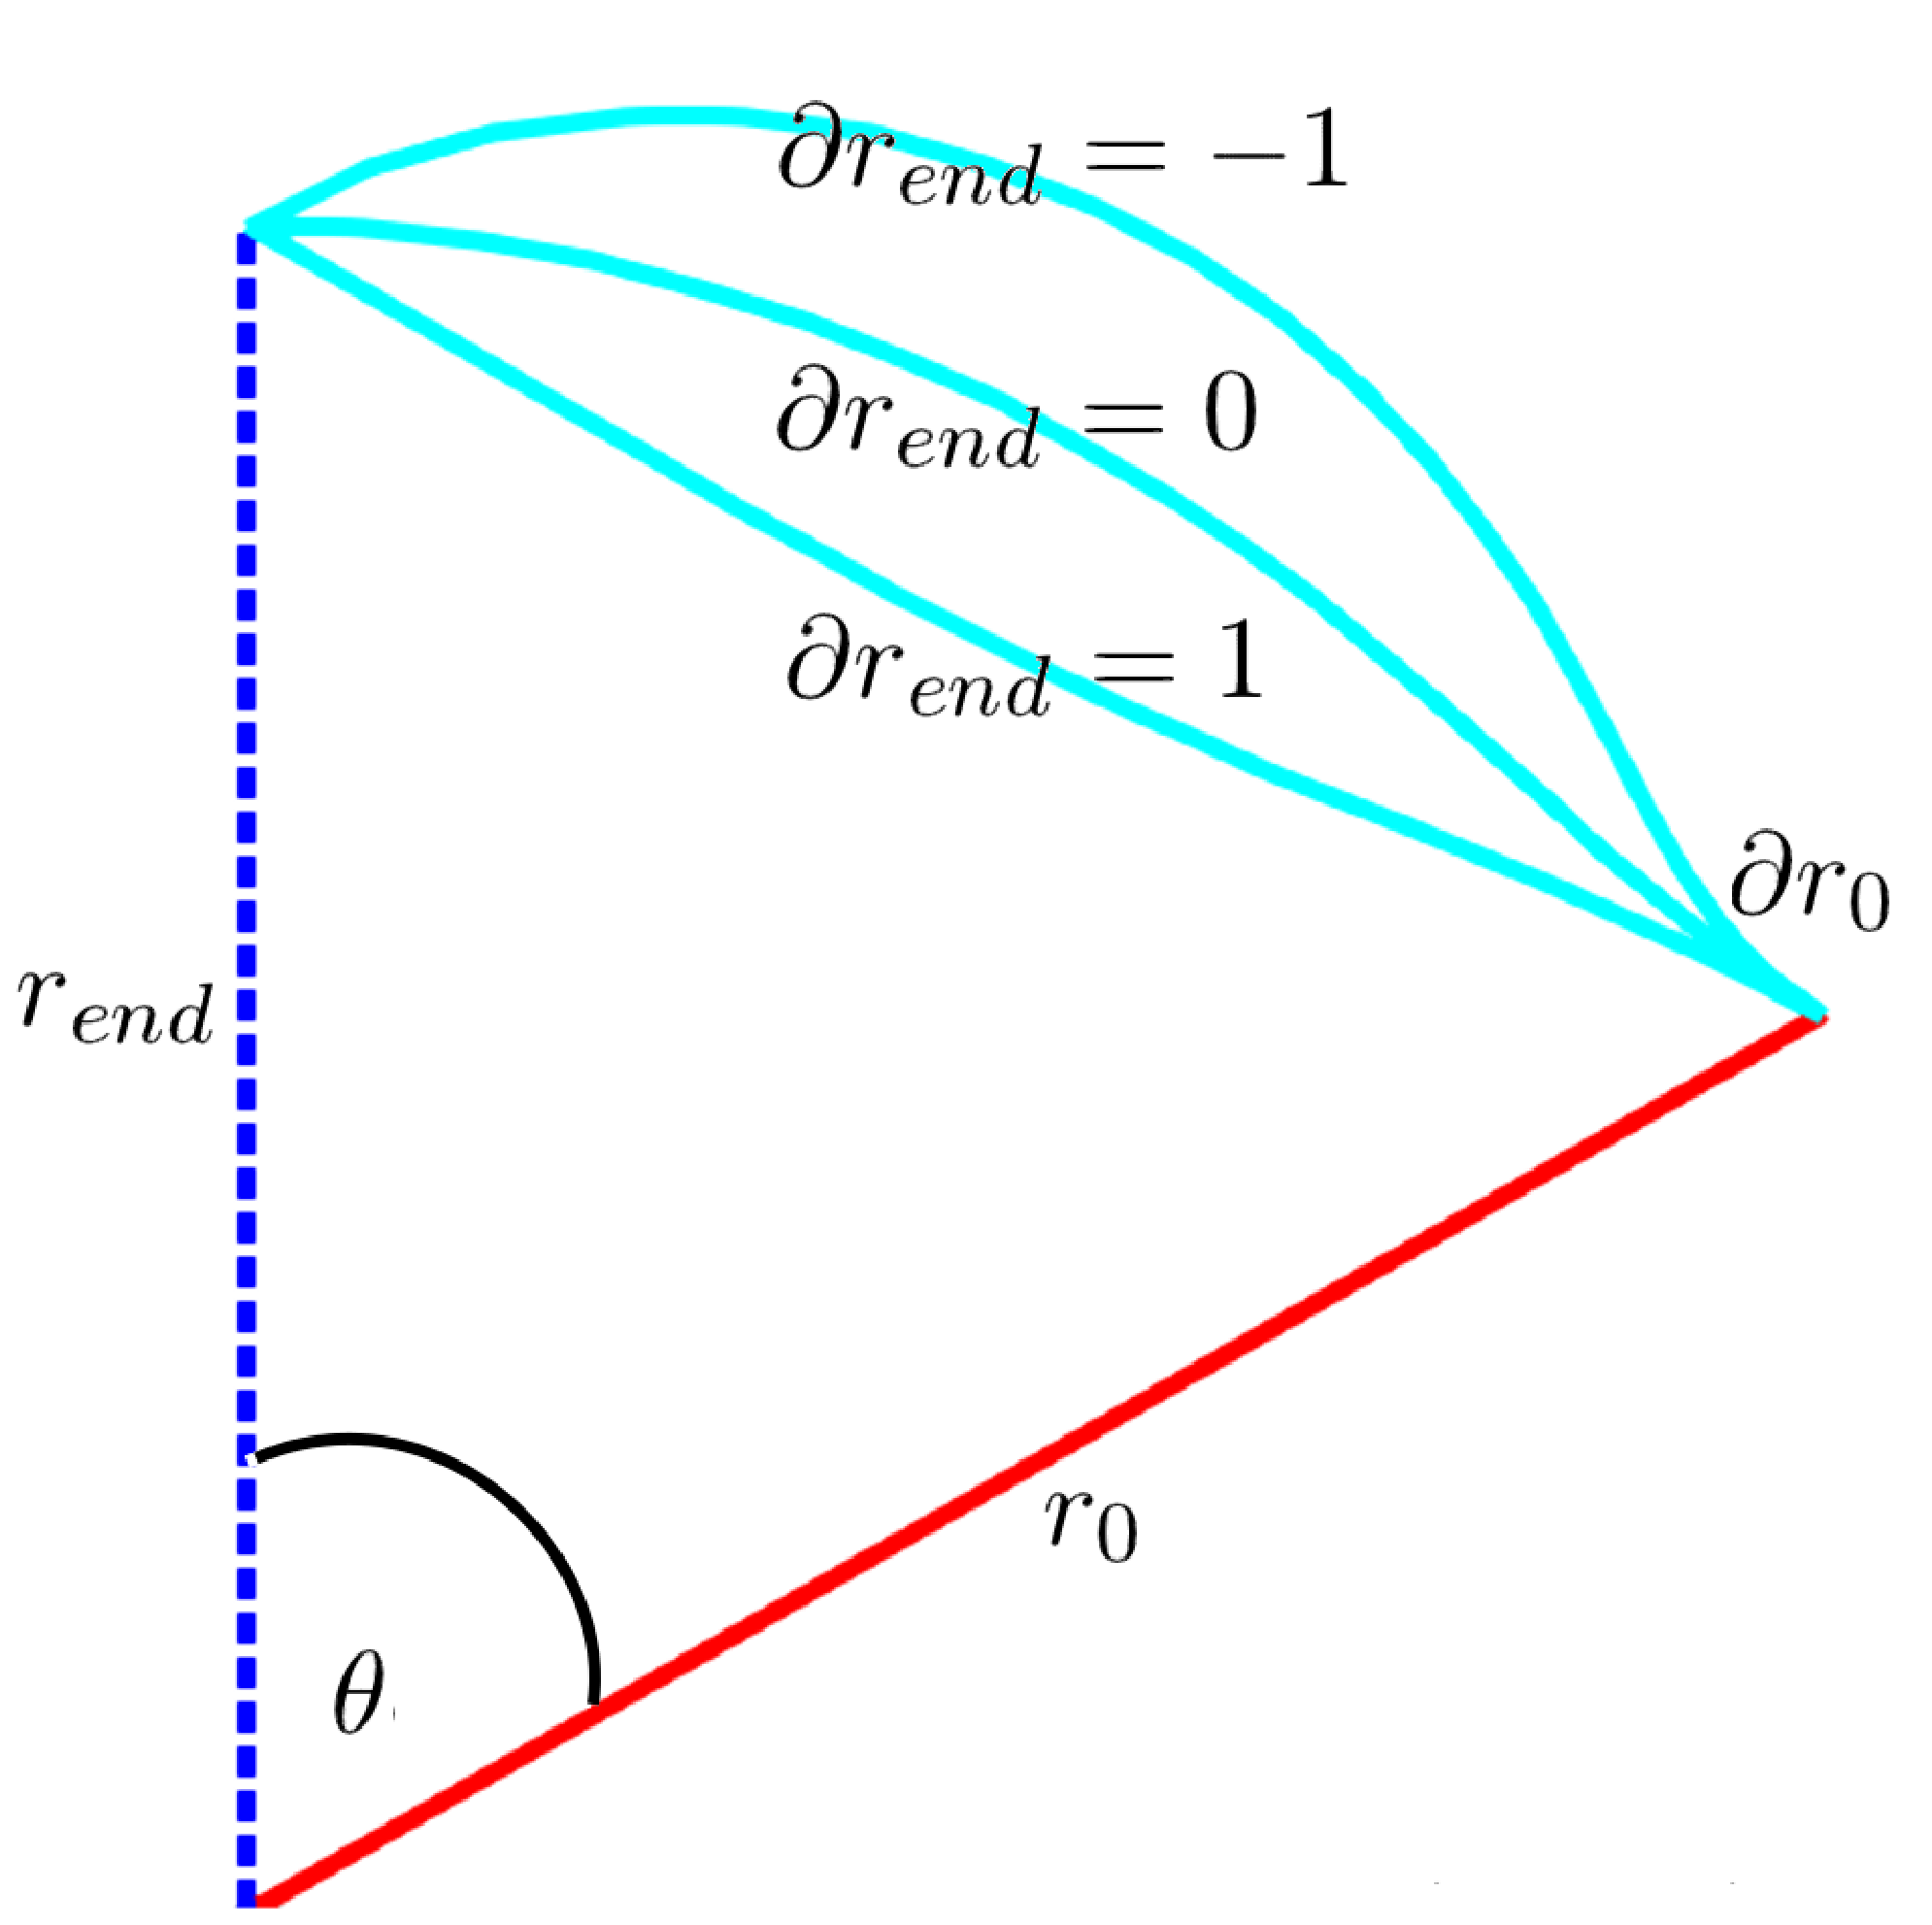
\epsfig{file = interpolationCrest0.eps, width =8cm}
 \caption[Radius interpolation.]{Radius interpolation showing the result for different $\partial r_{end}$.}
 \label{fig:interpolateRadius}  
\end{figure}

To produce space curves, the fitting is done for $[x, y, z]$ separately.
Using the discrete information given by the s-rep,
it is possible to retrieve $p_0$, $p_{end}$, and compute the discrete derivatives $\partial p_0$, and $\partial p_{end}$ 
which are the parameters to produce the fit.
To produce the crest curve, the crest atoms are considered to be on a loop 
where the crest positions are given by $cp_n$ where $n$ is the number of crest positions.
The directional derivatives are calculated as $\partial cp_j = (cp_{j + 1} - cp_{j - 1})/2$
which are projected onto the tangent plane given by the SS normal at each atom
$\partial \hat {cp_j} = \partial cp_j - (\partial cp_j \cdot N_{cp_j})N_{cp_j}$.
Figure \ref{fig:crestCurve} shows the interpolated crest as a space curve.

\begin{figure} 
 \centering  
 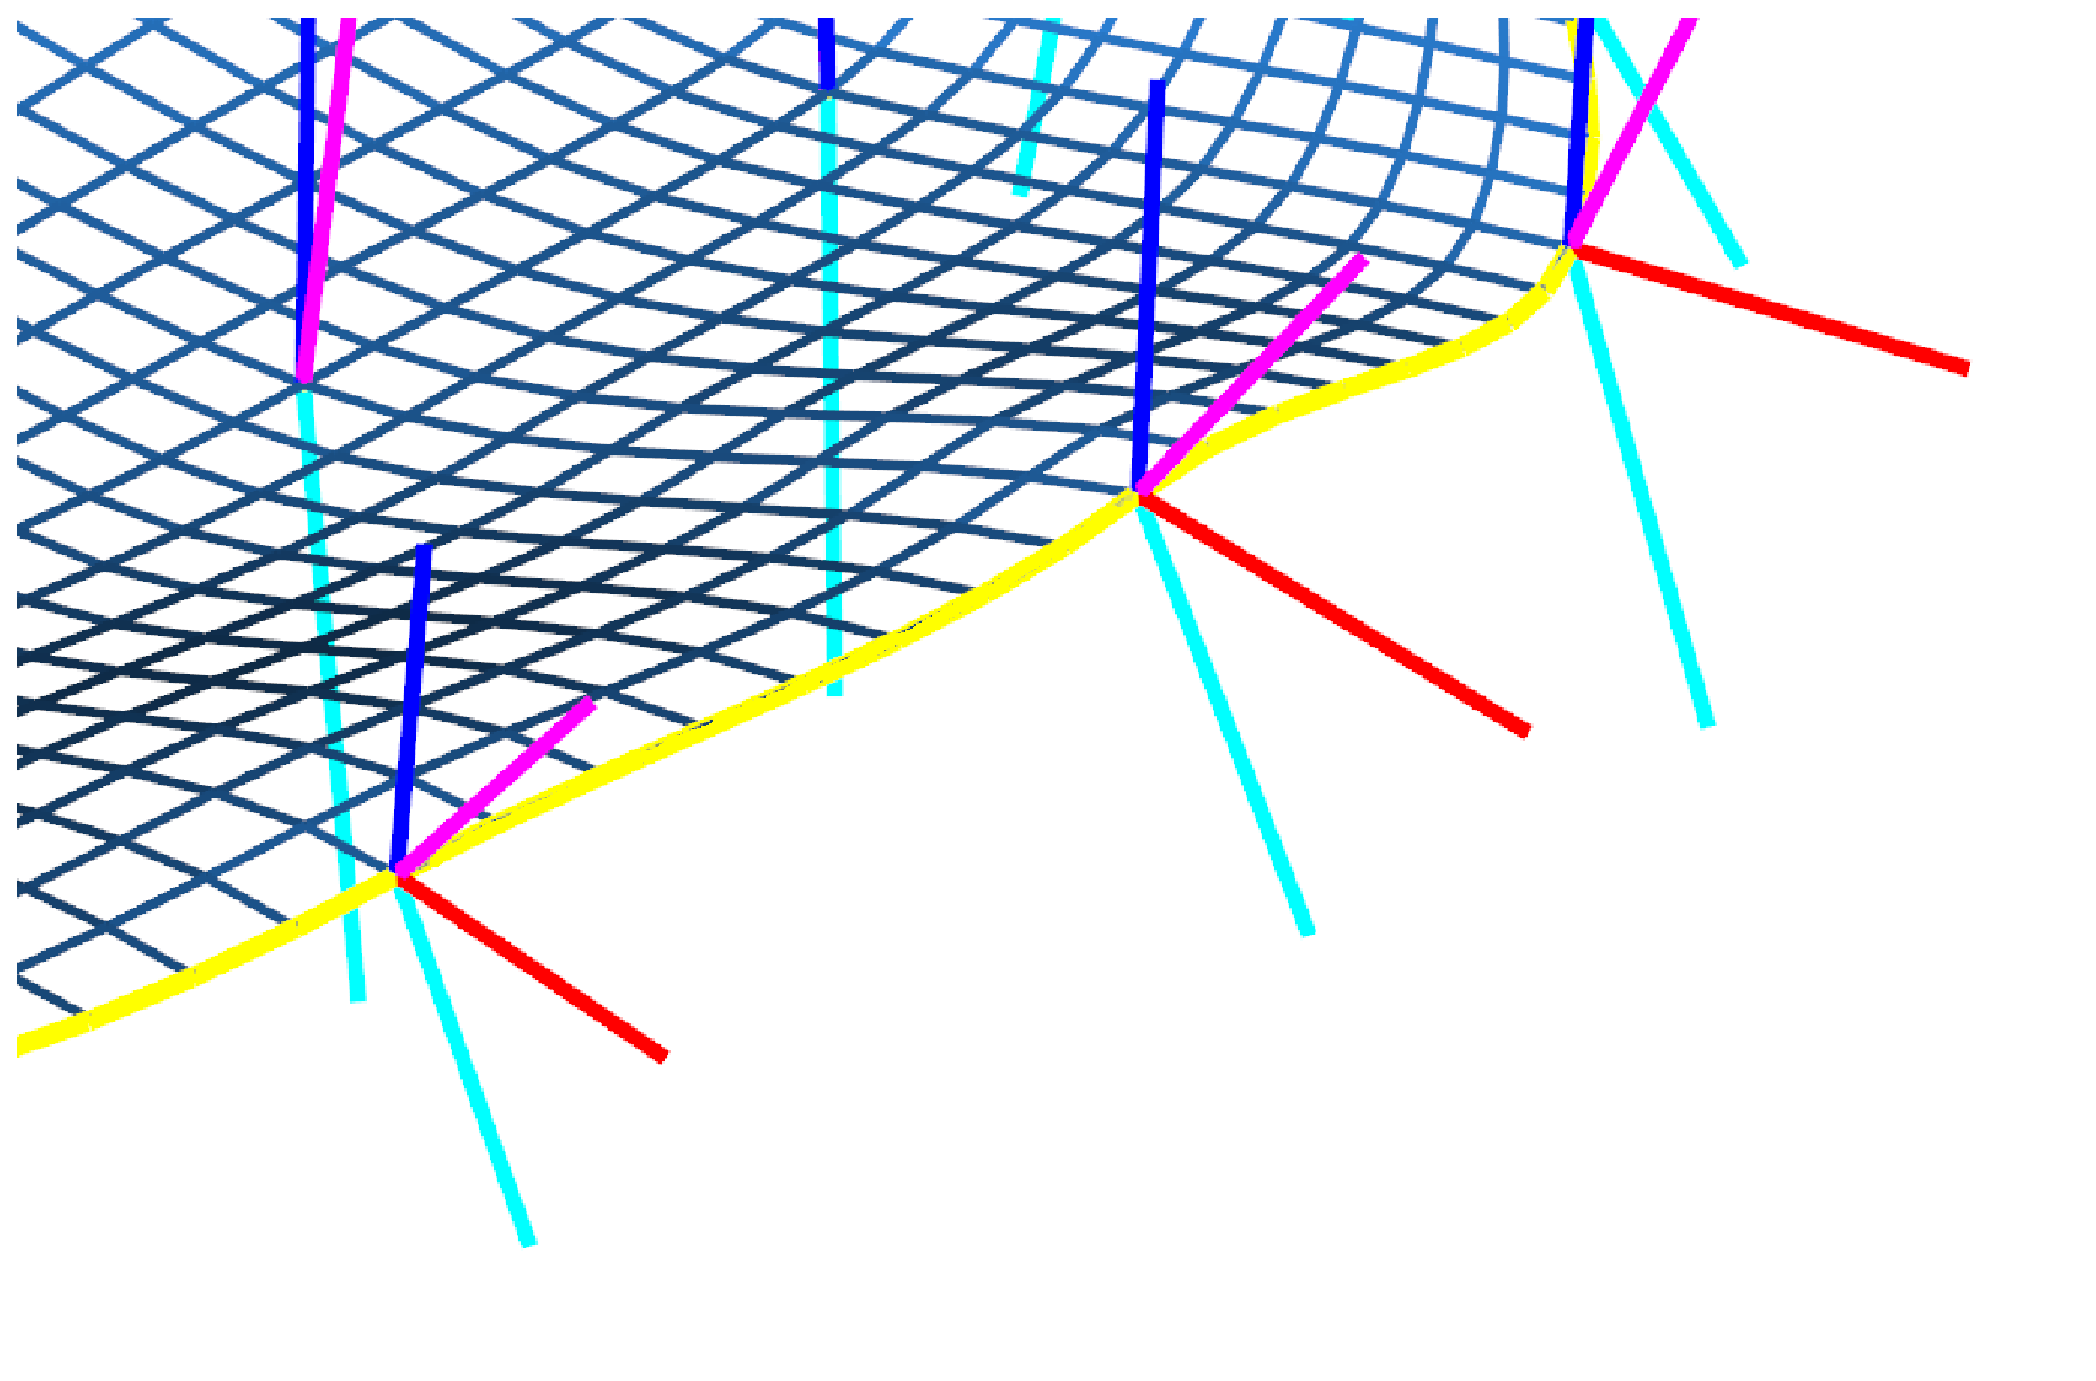
\epsfig{file = interpolationCrestCurve1.eps, width = 8cm}
 \caption[Interpolated crest curve.]{The interpolated crest curve is shown in yellow, using the crest positions to compute the directional derivatives and projecting the derivatives onto the tangent plane.}
 \label{fig:crestCurve}  
\end{figure}

\begin{figure} 
 \centering  
  \subfigure[Crest Spokes Top and Bottom]{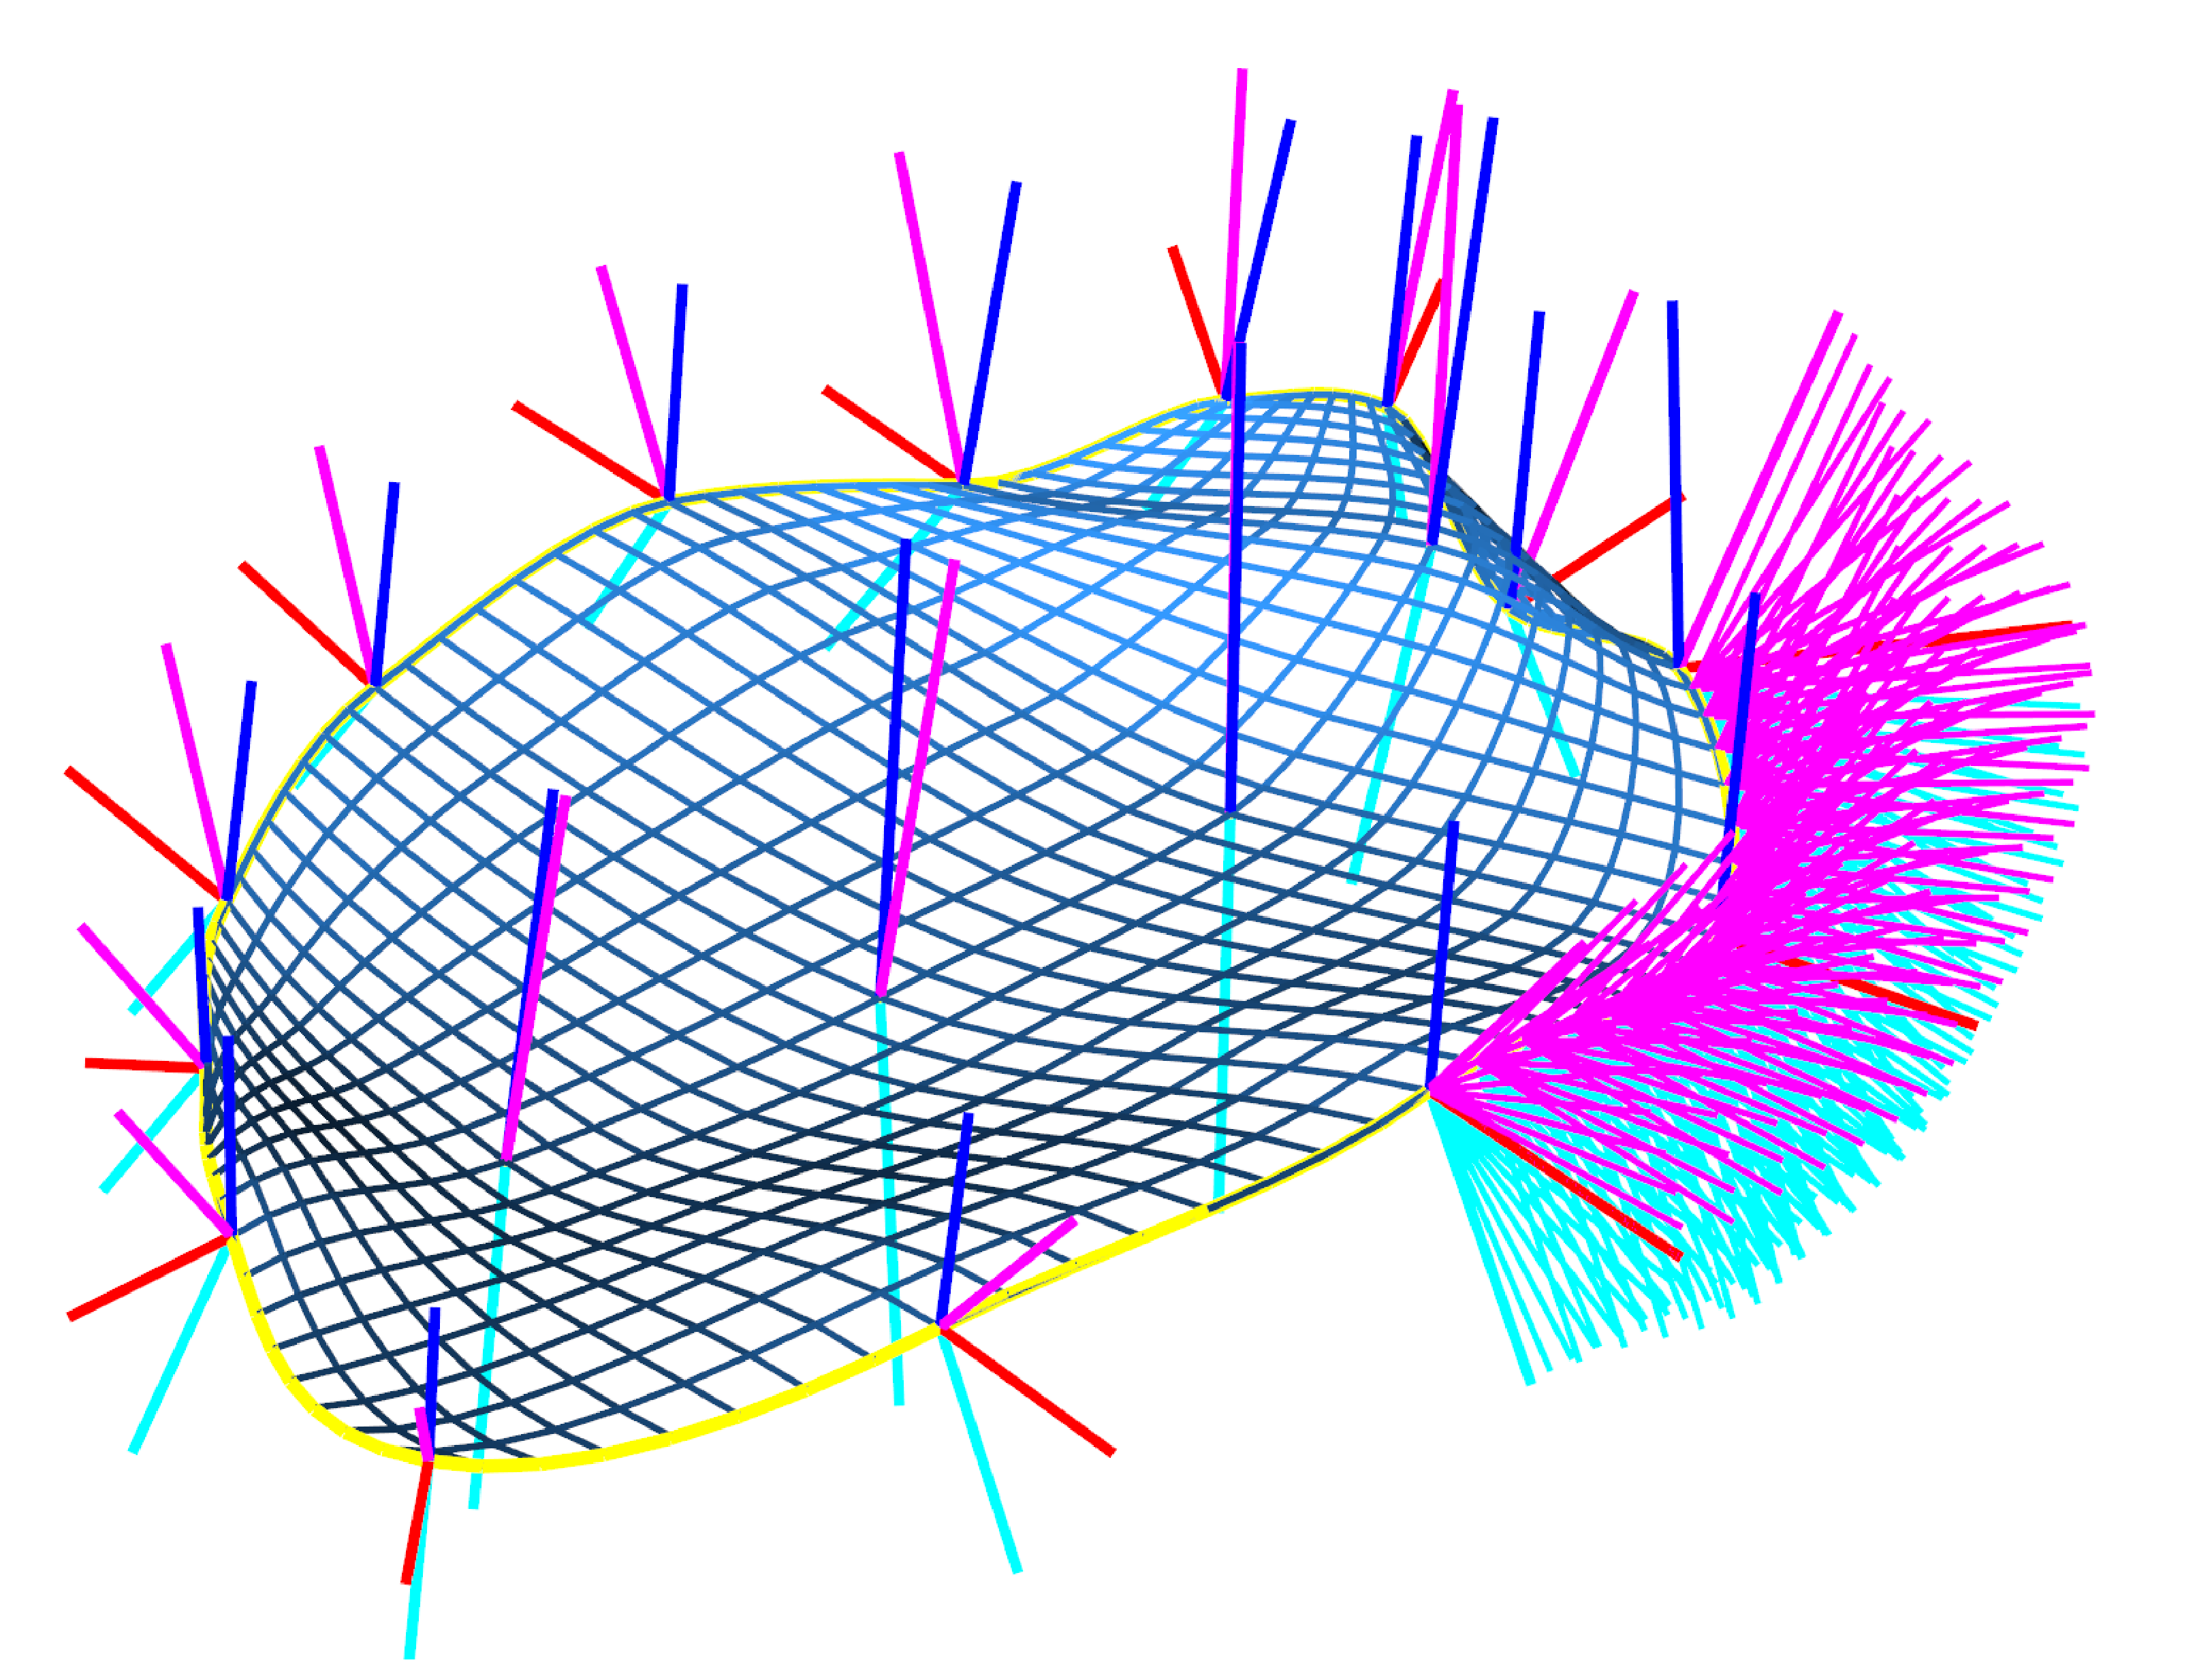
\epsfig{file = interpolationCrestSpokes.eps, width = 7cm}}
  \subfigure[Union of spokes to produce the crest]{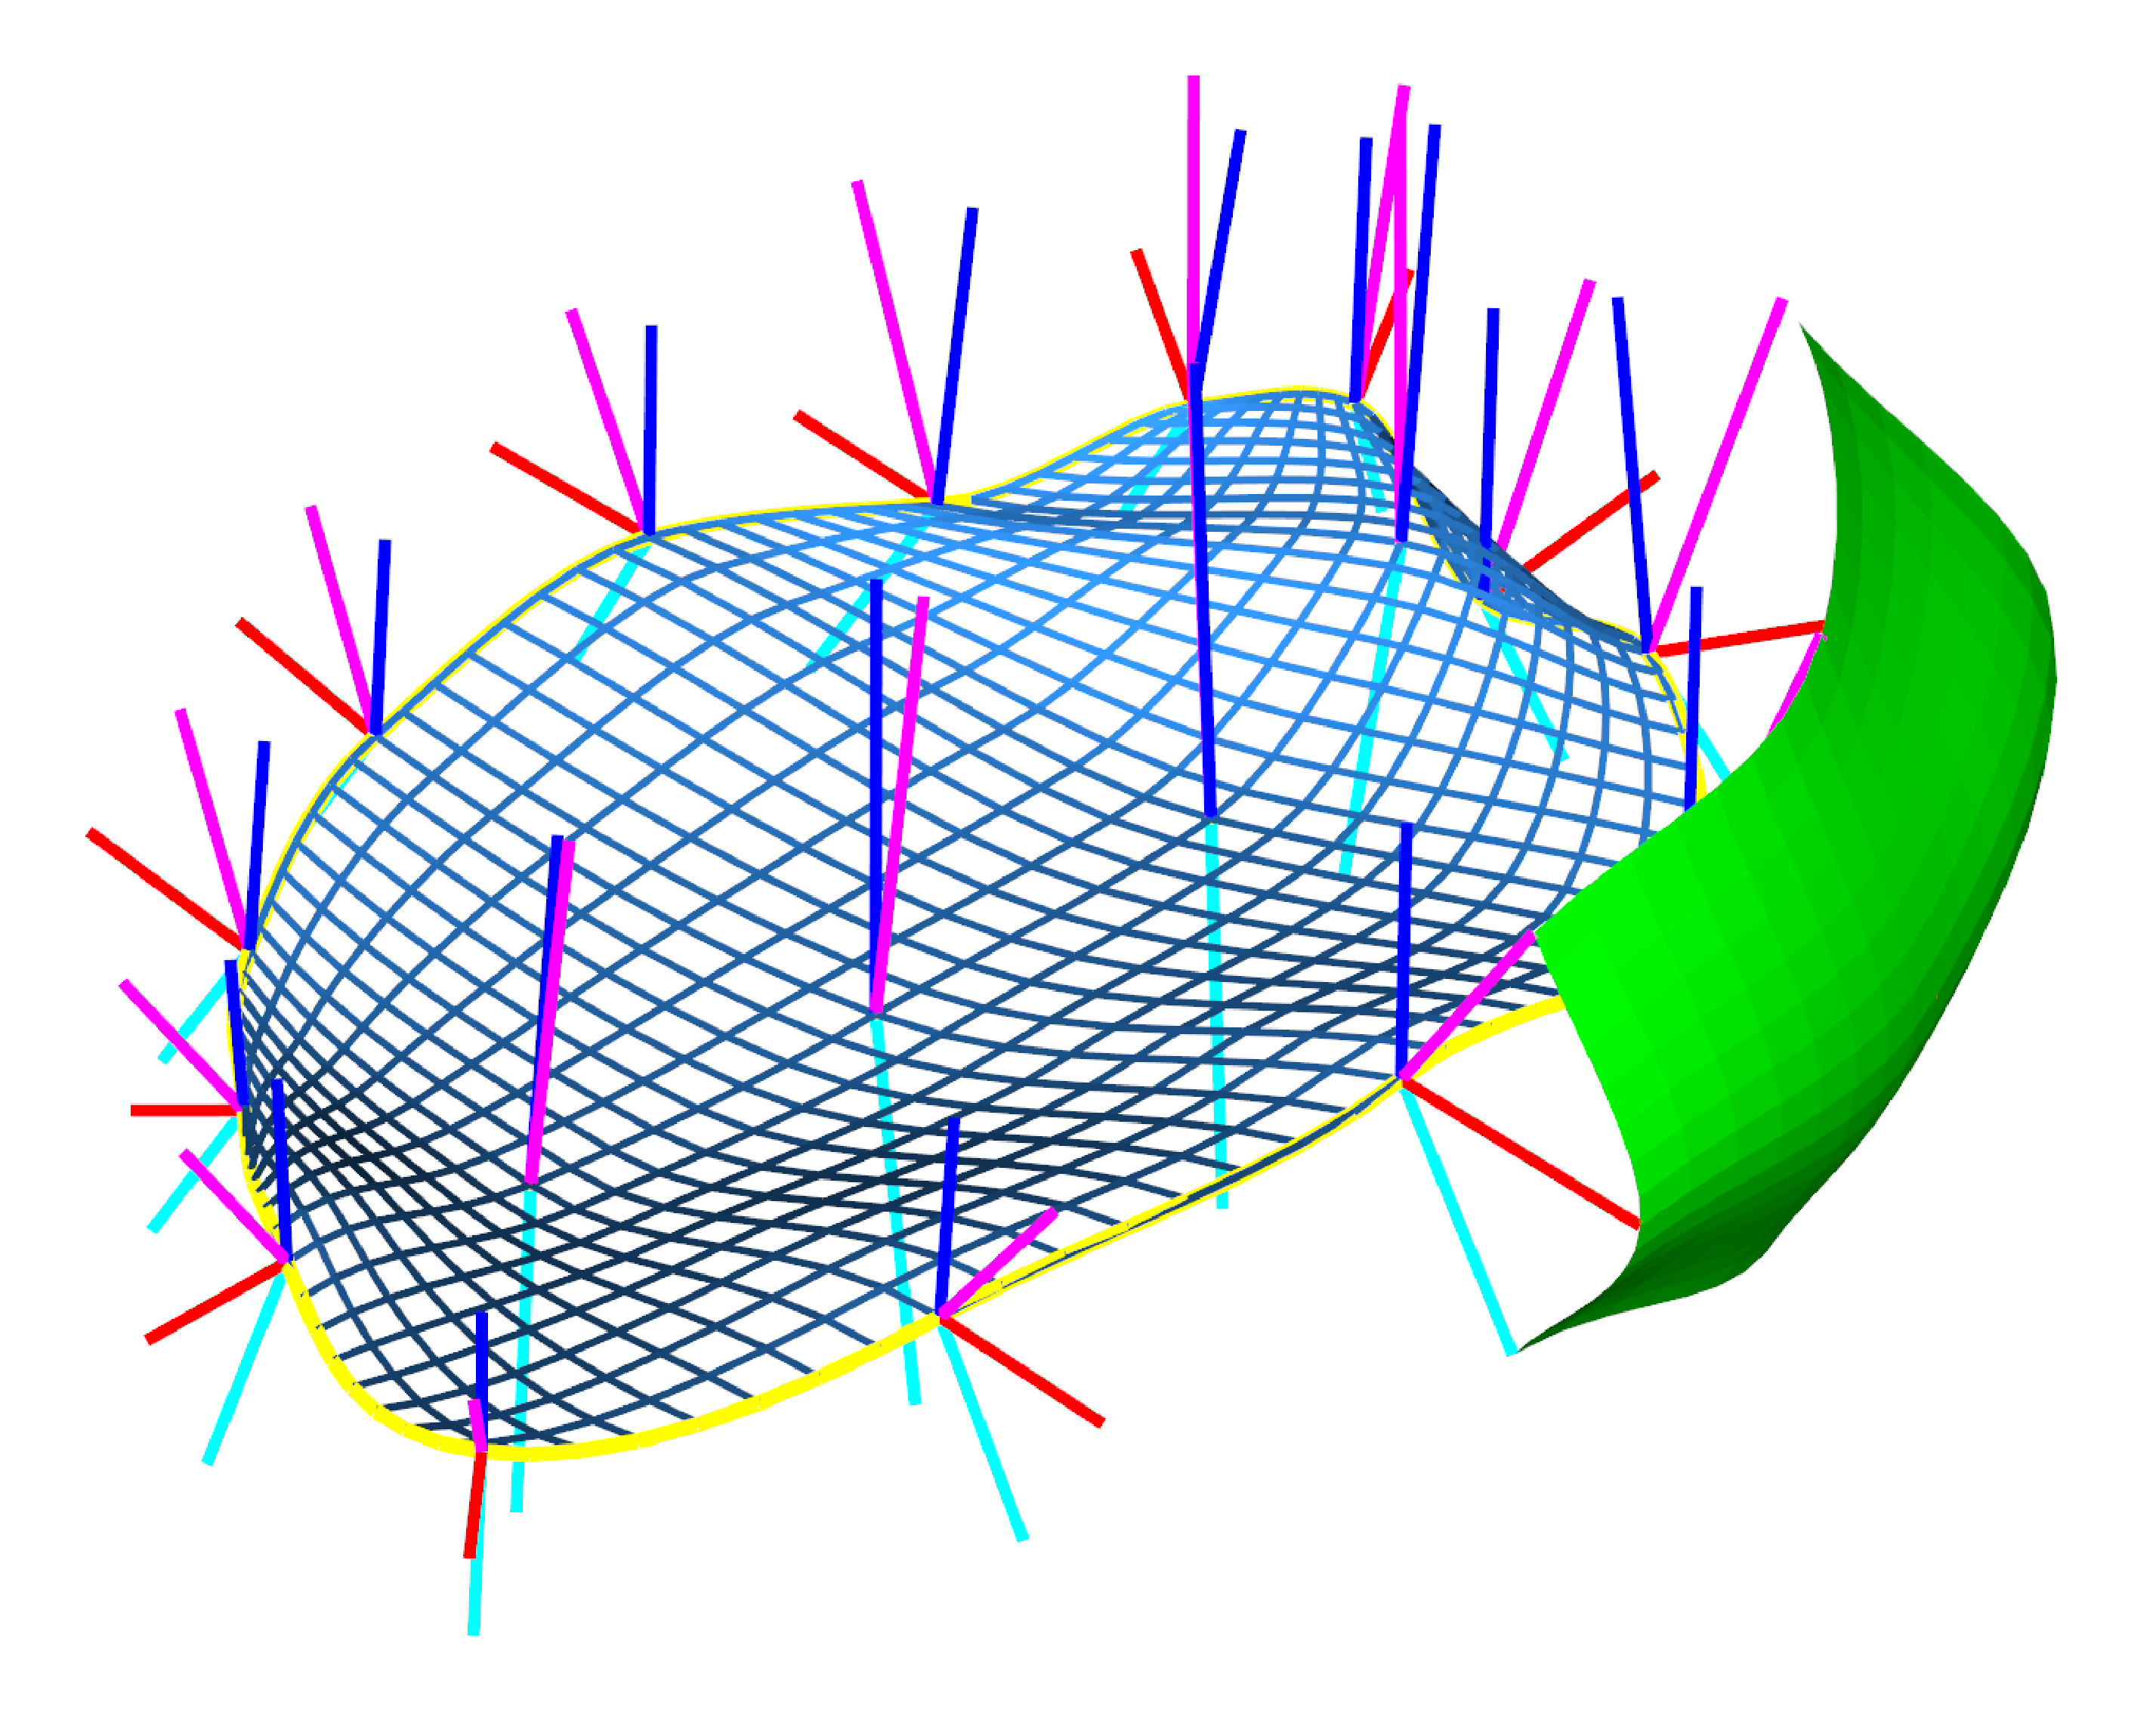
\epsfig{file = interpolationCrestSpokes0.eps, width = 7cm}}
 \caption[Slab's surfaces interpolation.]{The method interpolates top, crest and bottom spokes separately. 
	  A second interpolation is produced using the interpolated top, crest and bottom spokes in order to
	  join both sides of the object at the crest.}
 \label{fig:crestSpokes}  
\end{figure}

The same interpolation mechanism is used for top, crest and bottom spokes,
therefore, for a given $t$, 
it is possible to find the top spoke $CS(t)^1$, the crest spoke $CS(t)^0$ and the bottom spoke $CS(t)^{-1}$ 
plus the space curve to find the positions $Cp(t)$ where $t \in [0, 1]$ goes around 
the whole crest of the object. 

Finally we perform a second interpolation to generate the spokes from $top \rightarrow bottom$, which allows
us to produce the interpolated crest. 
Figure \ref{fig:crestSpokes} shows the interpolated spokes and the union of spokes forming a piece of the crest surface.
Figure \ref{fig:srepInterpolated} shows an example of the interpolated surface 
of an amygdala and the crest that joins both surfaces.

\begin{figure} 
 \centering  
 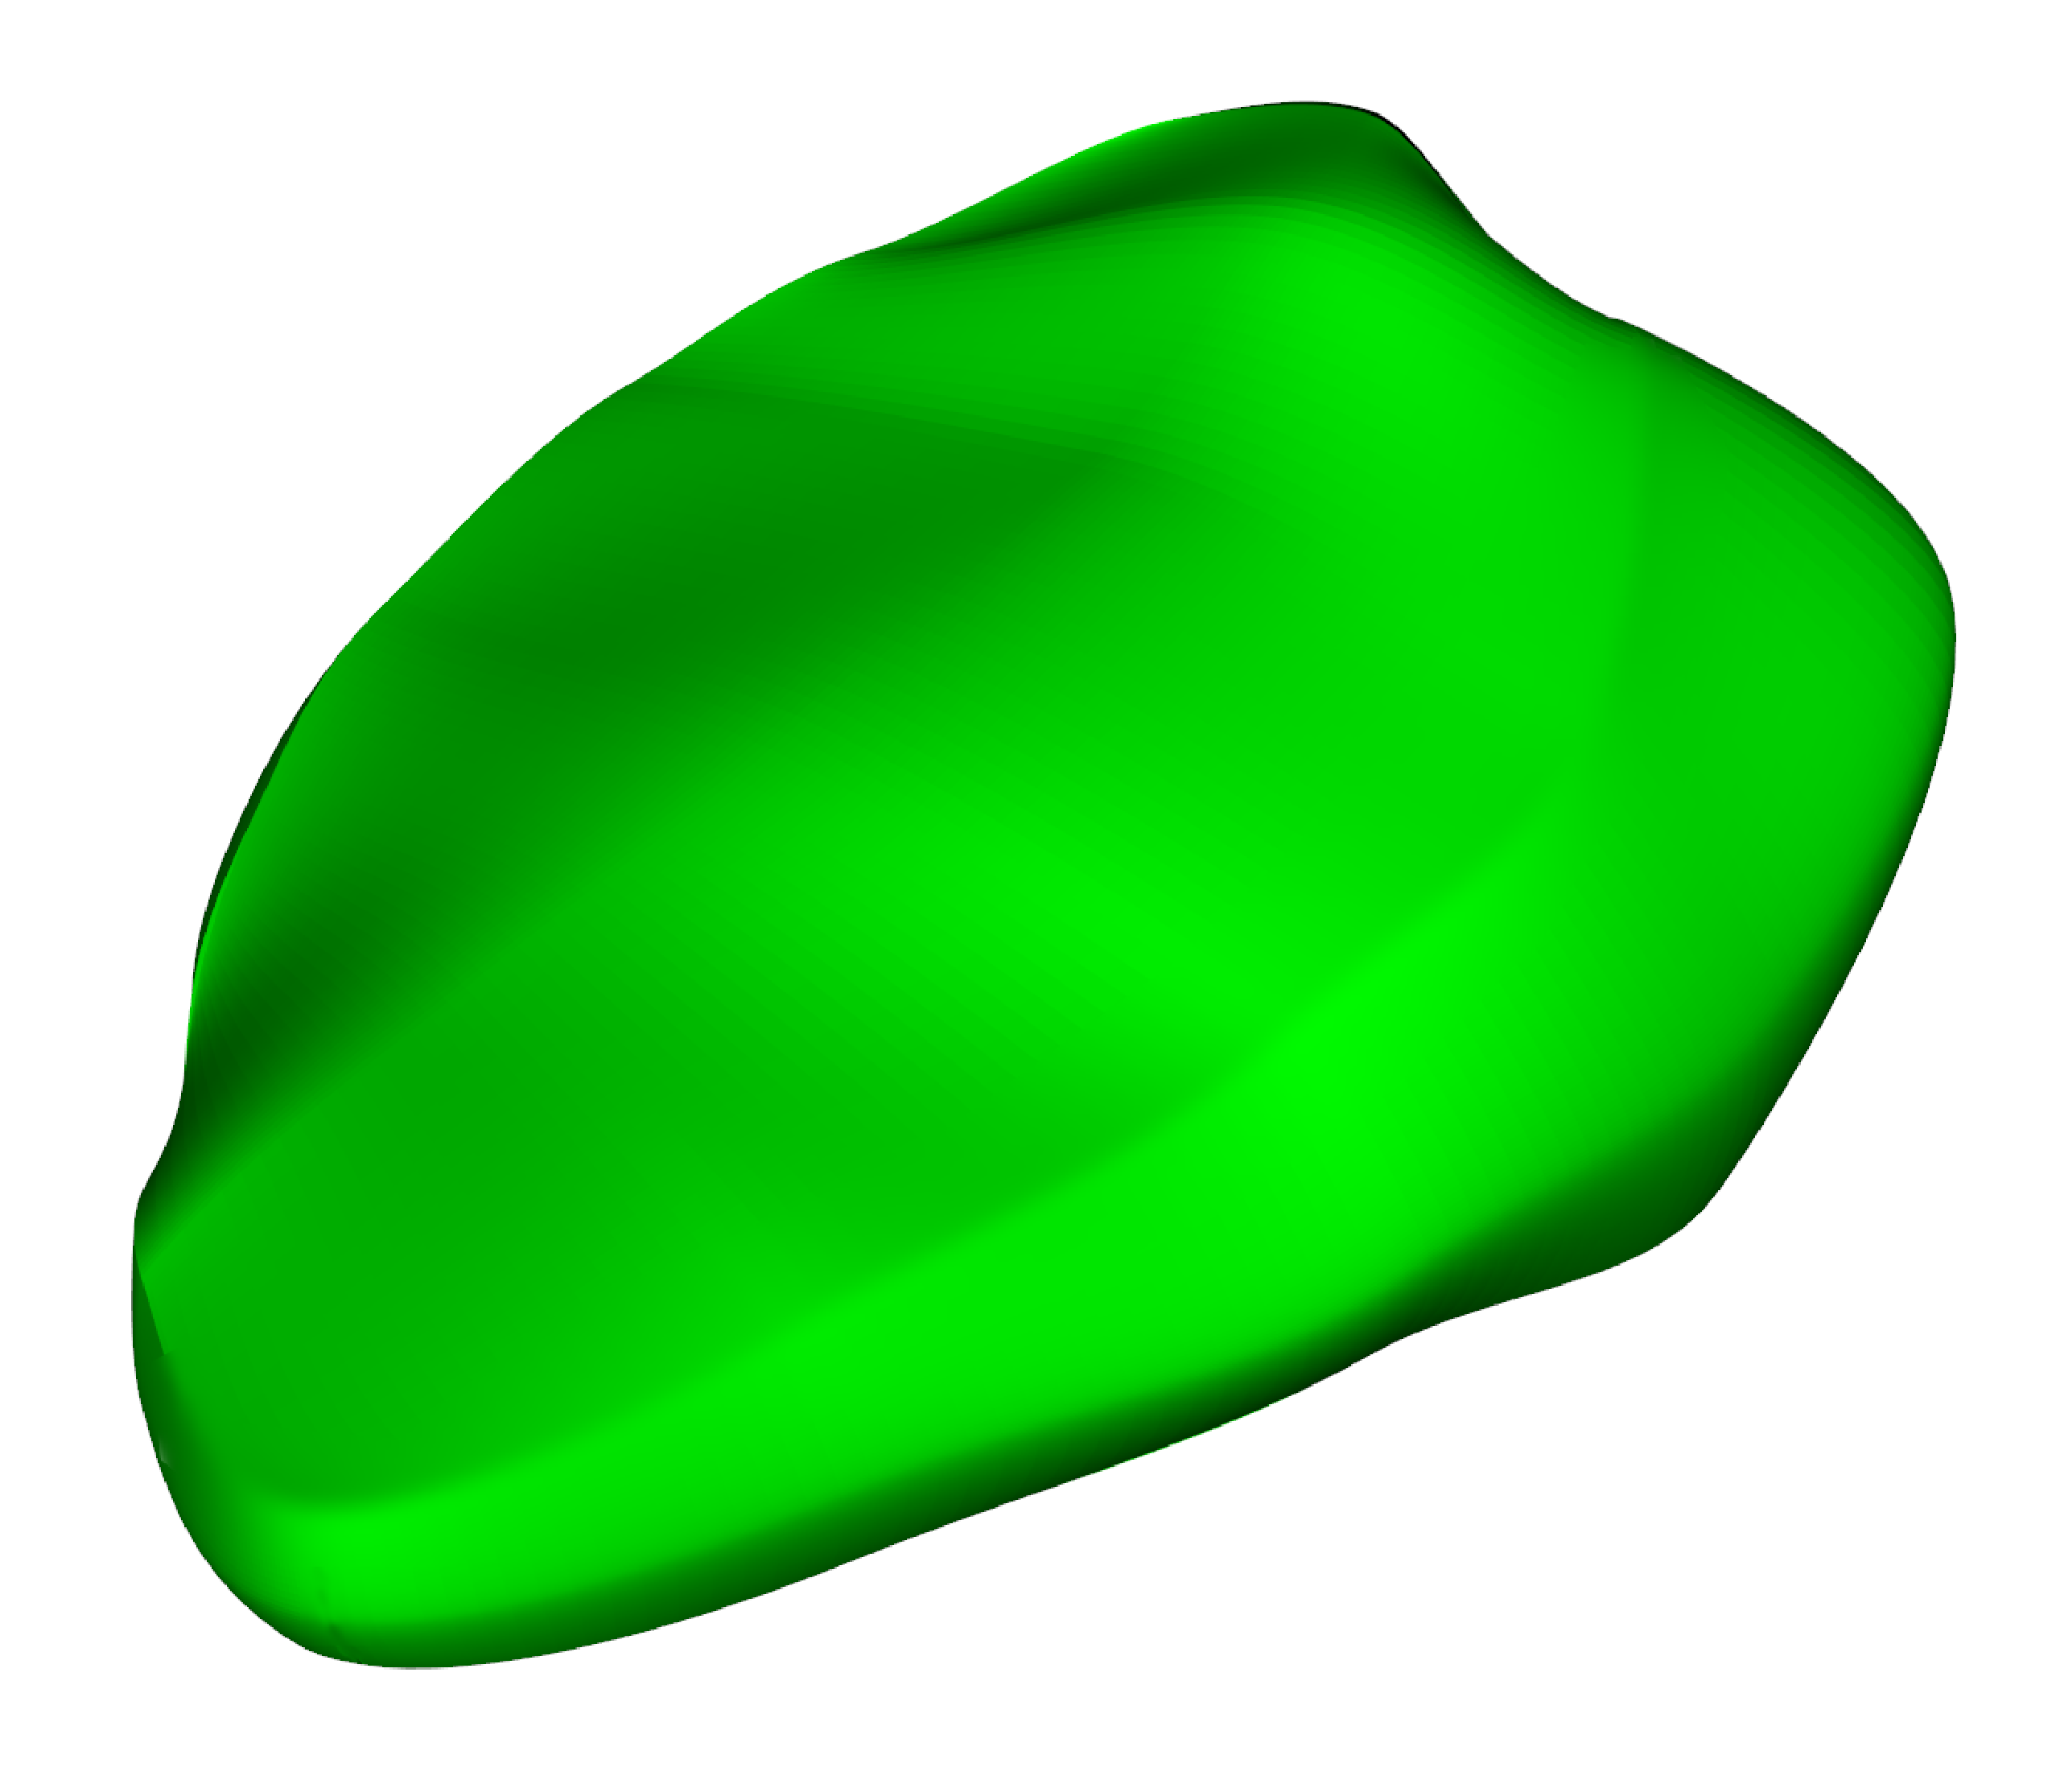
\epsfig{file = interpolationSrepSurface.eps, width = 8cm}
 \caption[Amygdala's s-rep.]{Complete s-rep of an amygdala, with top, bottom and crest surfaces. 
          The level of interpolation is higher to produce a smoother boundary.}
 \label{fig:srepInterpolated}  
\end{figure}

\subsubsection{Tubular objects} 

Different organs in the human body, 
such as blood vessels, the airways, and the intestines 
among many others are best represented using tubular structures.
Representing these objects with slab type s-reps is more difficult, 
because SS cannot be oriented in an intuitive manner. 
Instead, a parameterized space curve provides a more stable representation of a SS. 
Prominent authors such as \cite{binford1971visual}
proposed generalized cylinders, 
this method consists of a space curve, 
or axis, and a cross section function defined on the axis. For example, the function may be an ellipse. 
Another approach is the one proposed by \cite{huang1993generalized} named generalized tubes.
It is a two step approach, to segment and model tubular structures.
It starts with a local contour detection followed by a global 
recognition stage where the tube figures from the first stage are verified.
Such tube figures have been widely used on segmentation and modeling procedures,
but unfortunately, it is not trivial to include shape statistics using the approaches mentioned before;
such structures are best conceived to model individual tubes and not a population of them.
For this reason the tubular model proposed here is closely related 
to quasi-tubes, a model proposed by \cite{saboomedial}.

\begin{figure} 
 \centering  
  \subfigure[Interpolated spokes of a tube figure, the MA is shown in yellow and the spokes in cyan.
             The MA is parameterized by a single parameter $u$, while the spokes on the MA are parameterized by $(u, \phi)$, 
             $\tau$ represents the portion of the spoke from the MA to the boundary.]{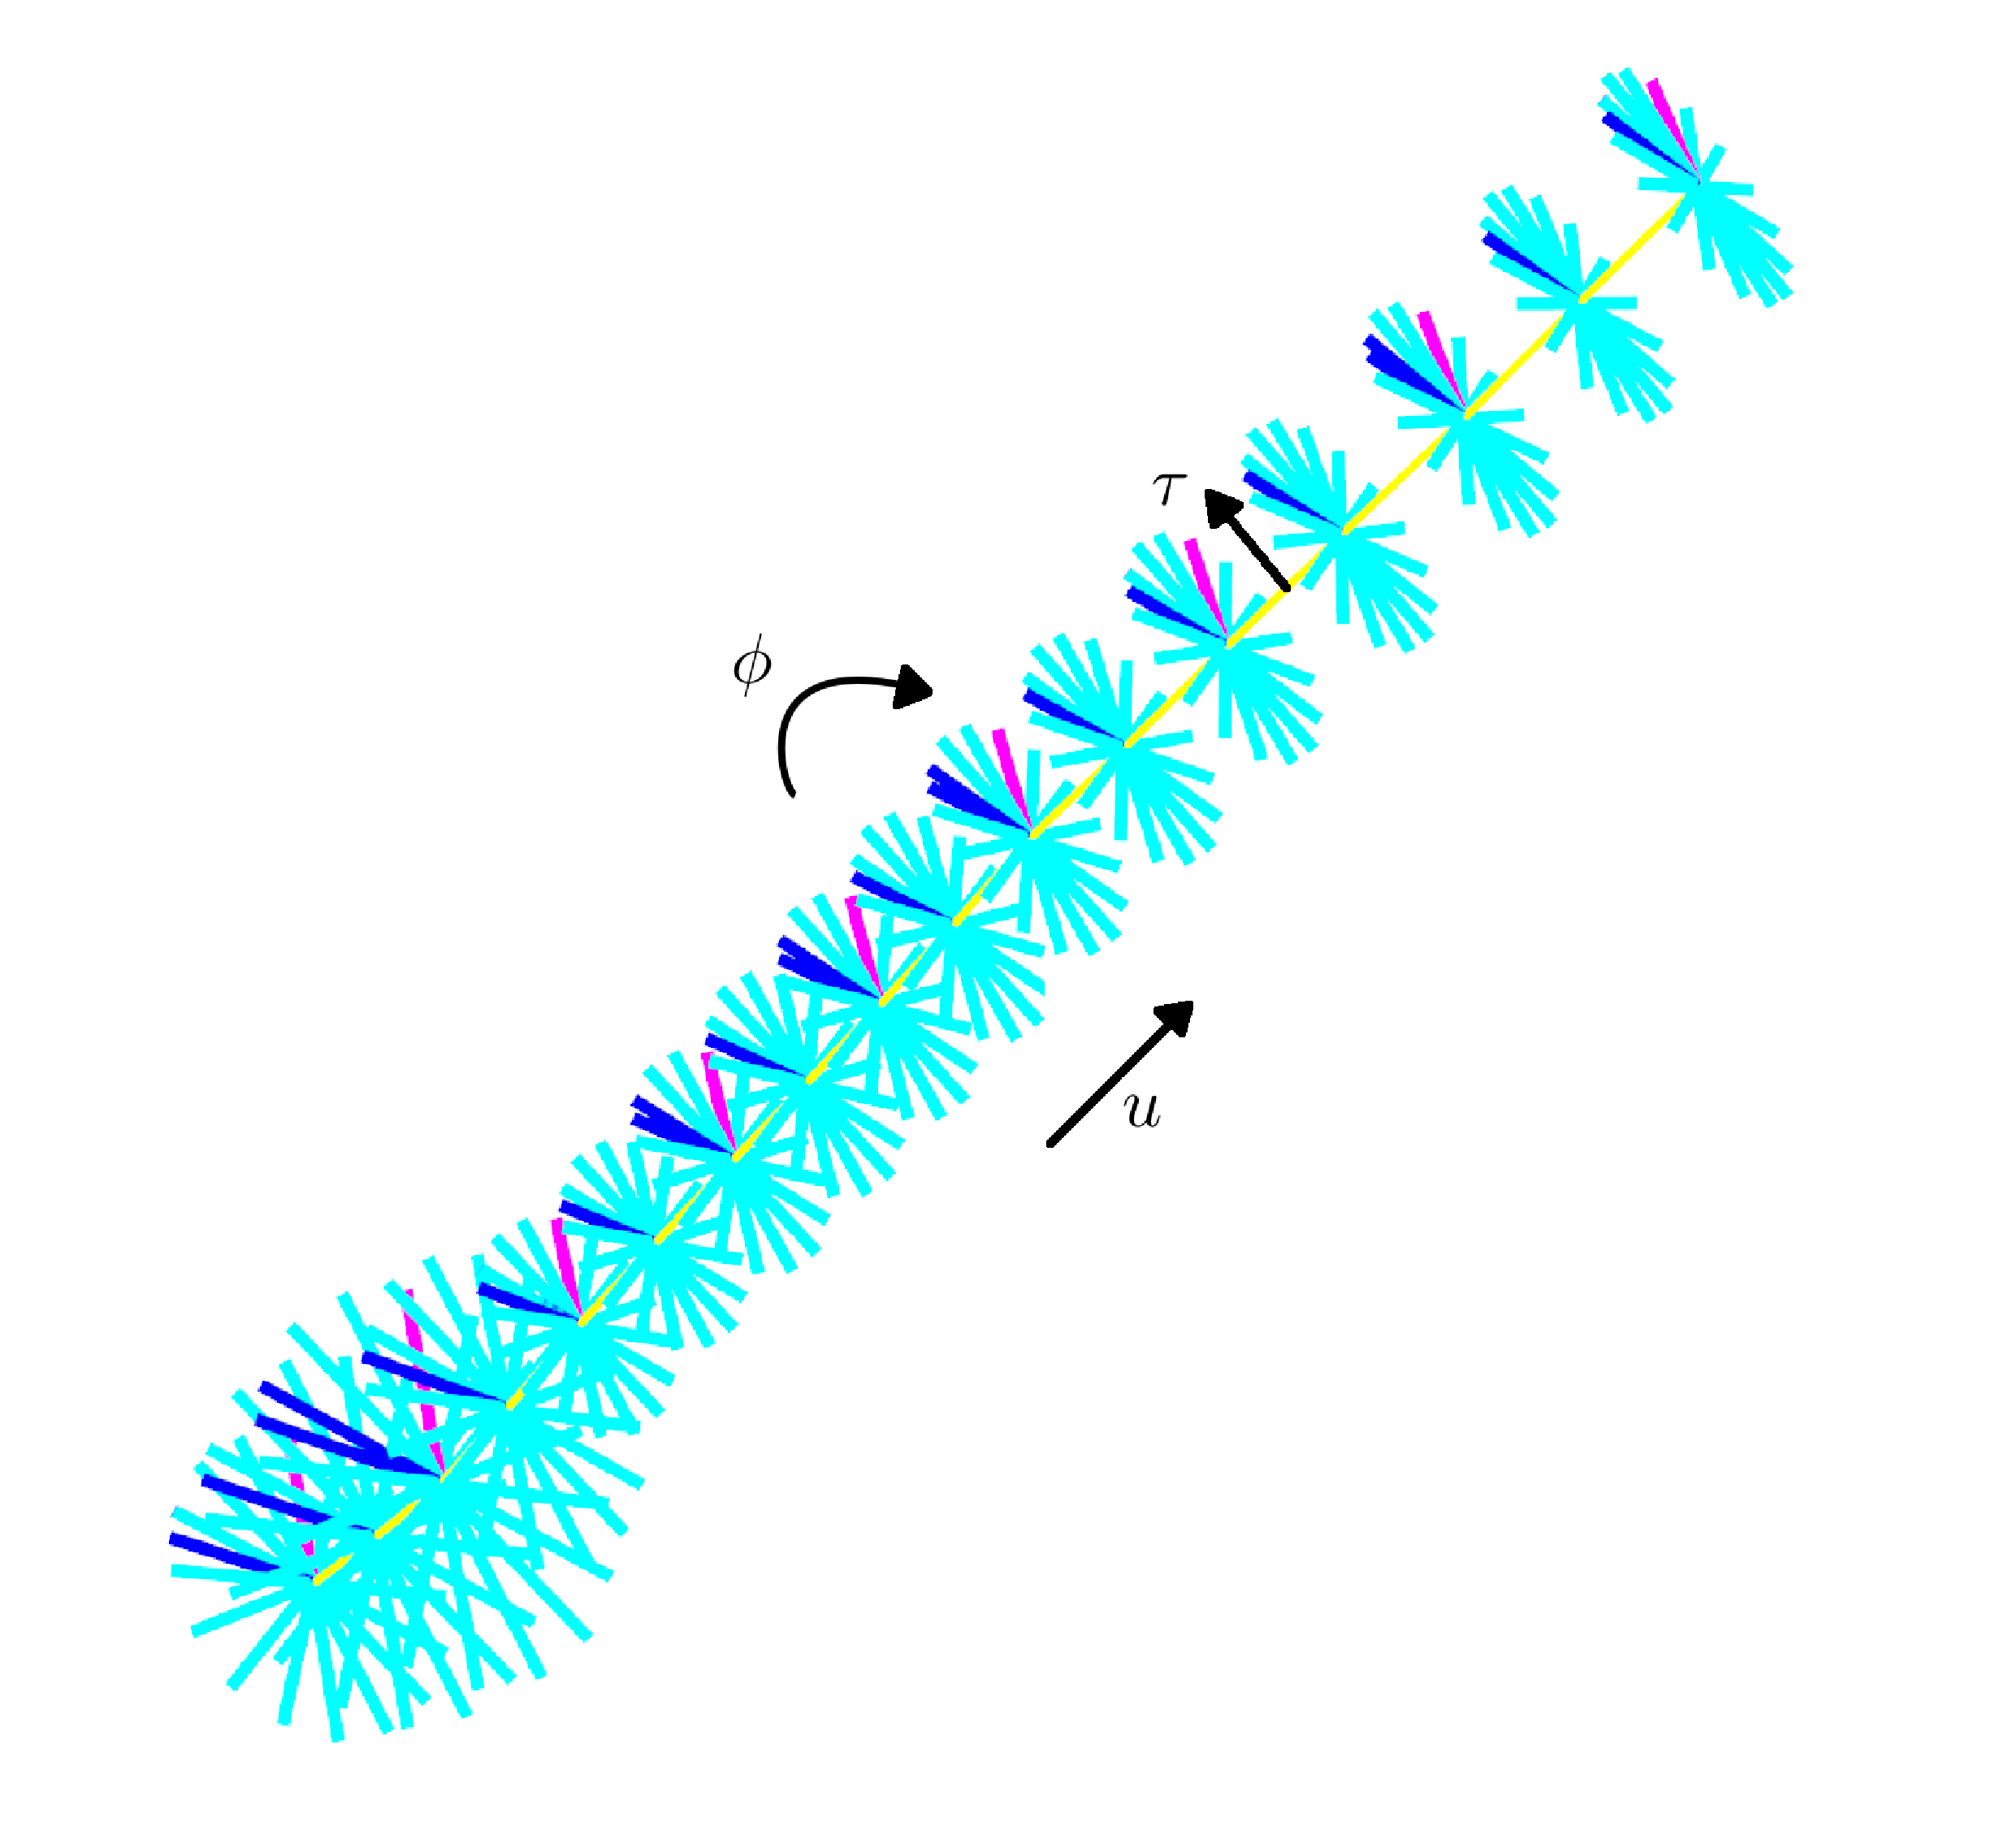
\epsfig{file = interpolationTube0.eps, width = 6cm}}
  \subfigure[The union of spoke tips produce the boundary of the tubular object]{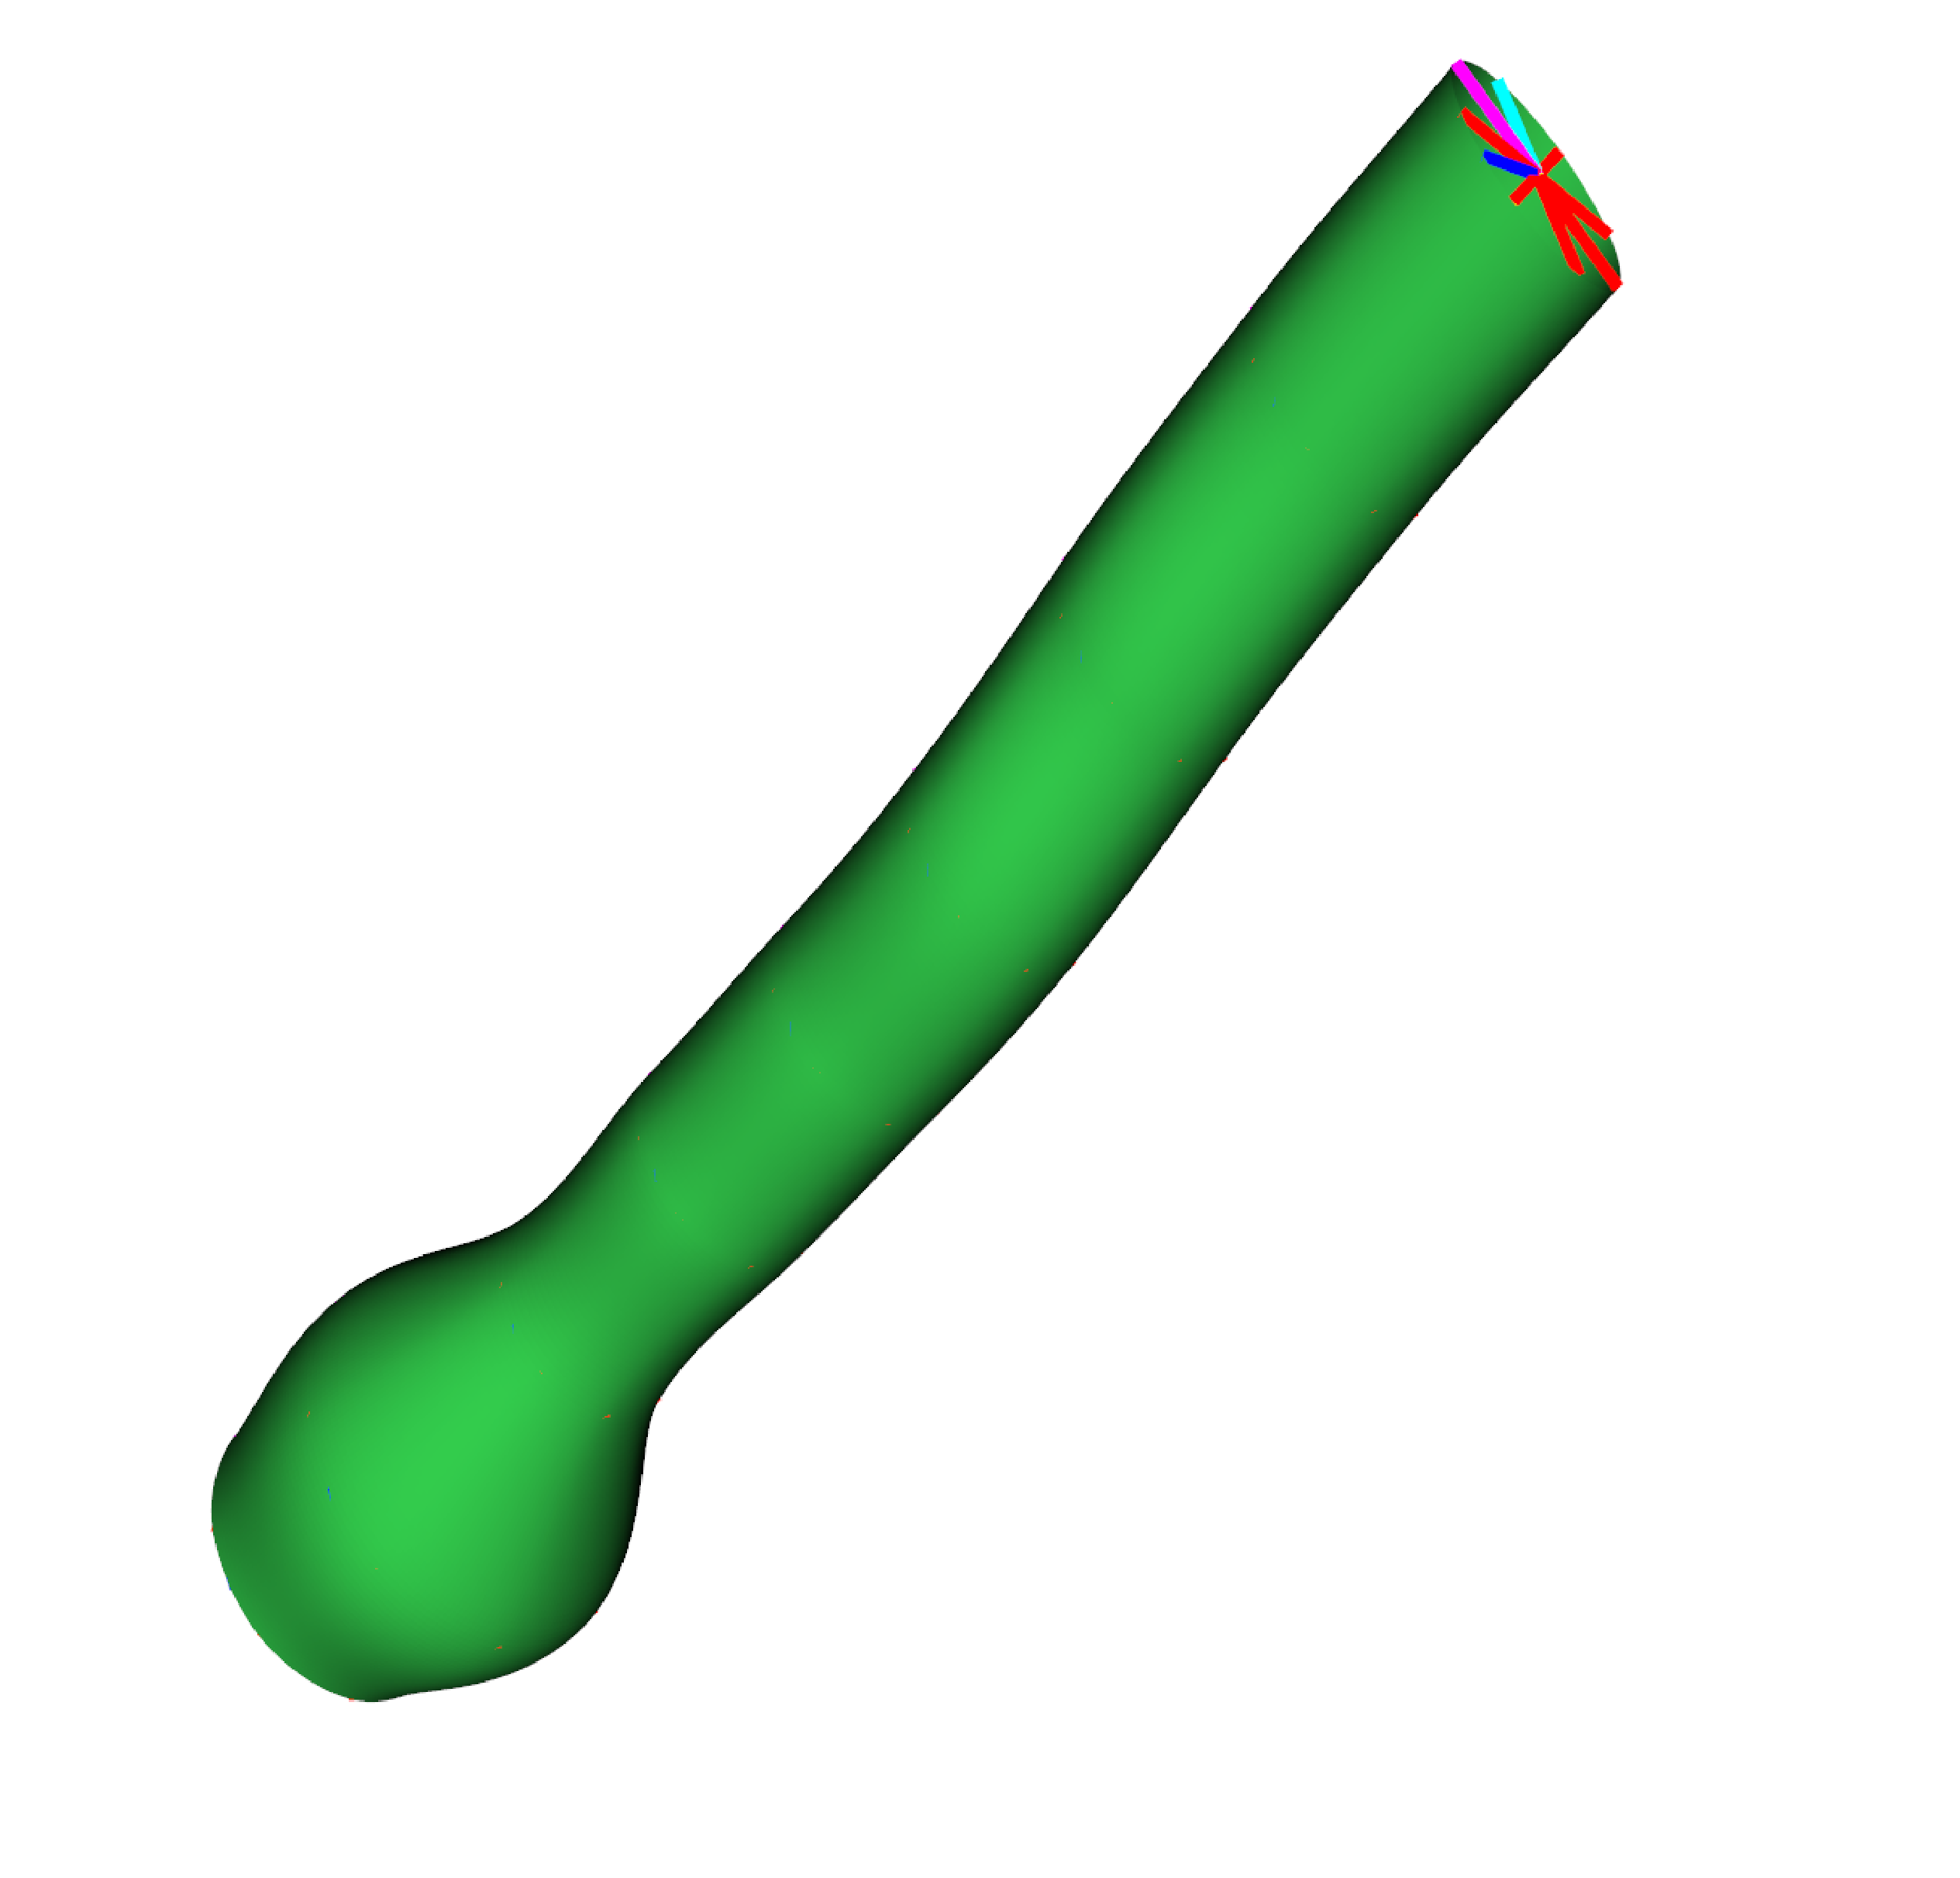
\epsfig{file = interpolationTube1.eps, width = 6cm}}
 \caption[Quasi-tube interpolation.]{The crest interpolation method is also capable of interpolating tube figures.}
 \label{fig:tubular}  
\end{figure} 

Figure  \ref{fig:tubular} shows the result of the interpolation using the same 
formulation from the crest method. 
These quasi-tubes are defined in the same manner as s-reps, $S_{rep} = \{p_i, S_i\}$; 
the difference is that the spokes are all placed following a space curve that 
defines the MA, and the interpolation is done with the spokes that share the same hub.
They are differentiated by the angle $\phi$ from 
the spoke located at $\phi = 0$ which is highlighted in magenta. 

Since the definition of this tubular object is equivalent to 
the definition of an s-rep, 
the statistical framework CPNS 
is also compatible. 
However, tubular objects are not widely used in this dissertation and
will be reserved for future work. 

The last subject that is addressed on geometric representation
is the internal coordinates of an object.

\subsection{Internal coordinates of an object}
\label{sec:internalCoordinates}

The internal coordinates of an object are described by $X2U$ maps. 
The mapping enables querying world coordinates to find object coordinates.
$X2U$ maps will be used in Chapter \ref{chapter:MRISimulation}
to map the solids generated in Chapter \ref{chapter:textureSynthesis} 
to an s-rep. This is possible since the solids are synthesized 
in a cube. Each coordinates in the cube can be related to $[u, v, \tau]$, thus, providing 
a simple mechanism to map a solid to an object. 

The amygdala shown in Figure \ref{fig:srepInterpolated} 
is composed by 18 atoms placed on a double sided grid $(m, n) = (6, 3)$, where every spoke's tail is placed.
The total number of spokes is 26 and
in order to give
a unique coordinate to every spoke, 
the MS is unfolded. 

\begin{figure} 
 \centering  
 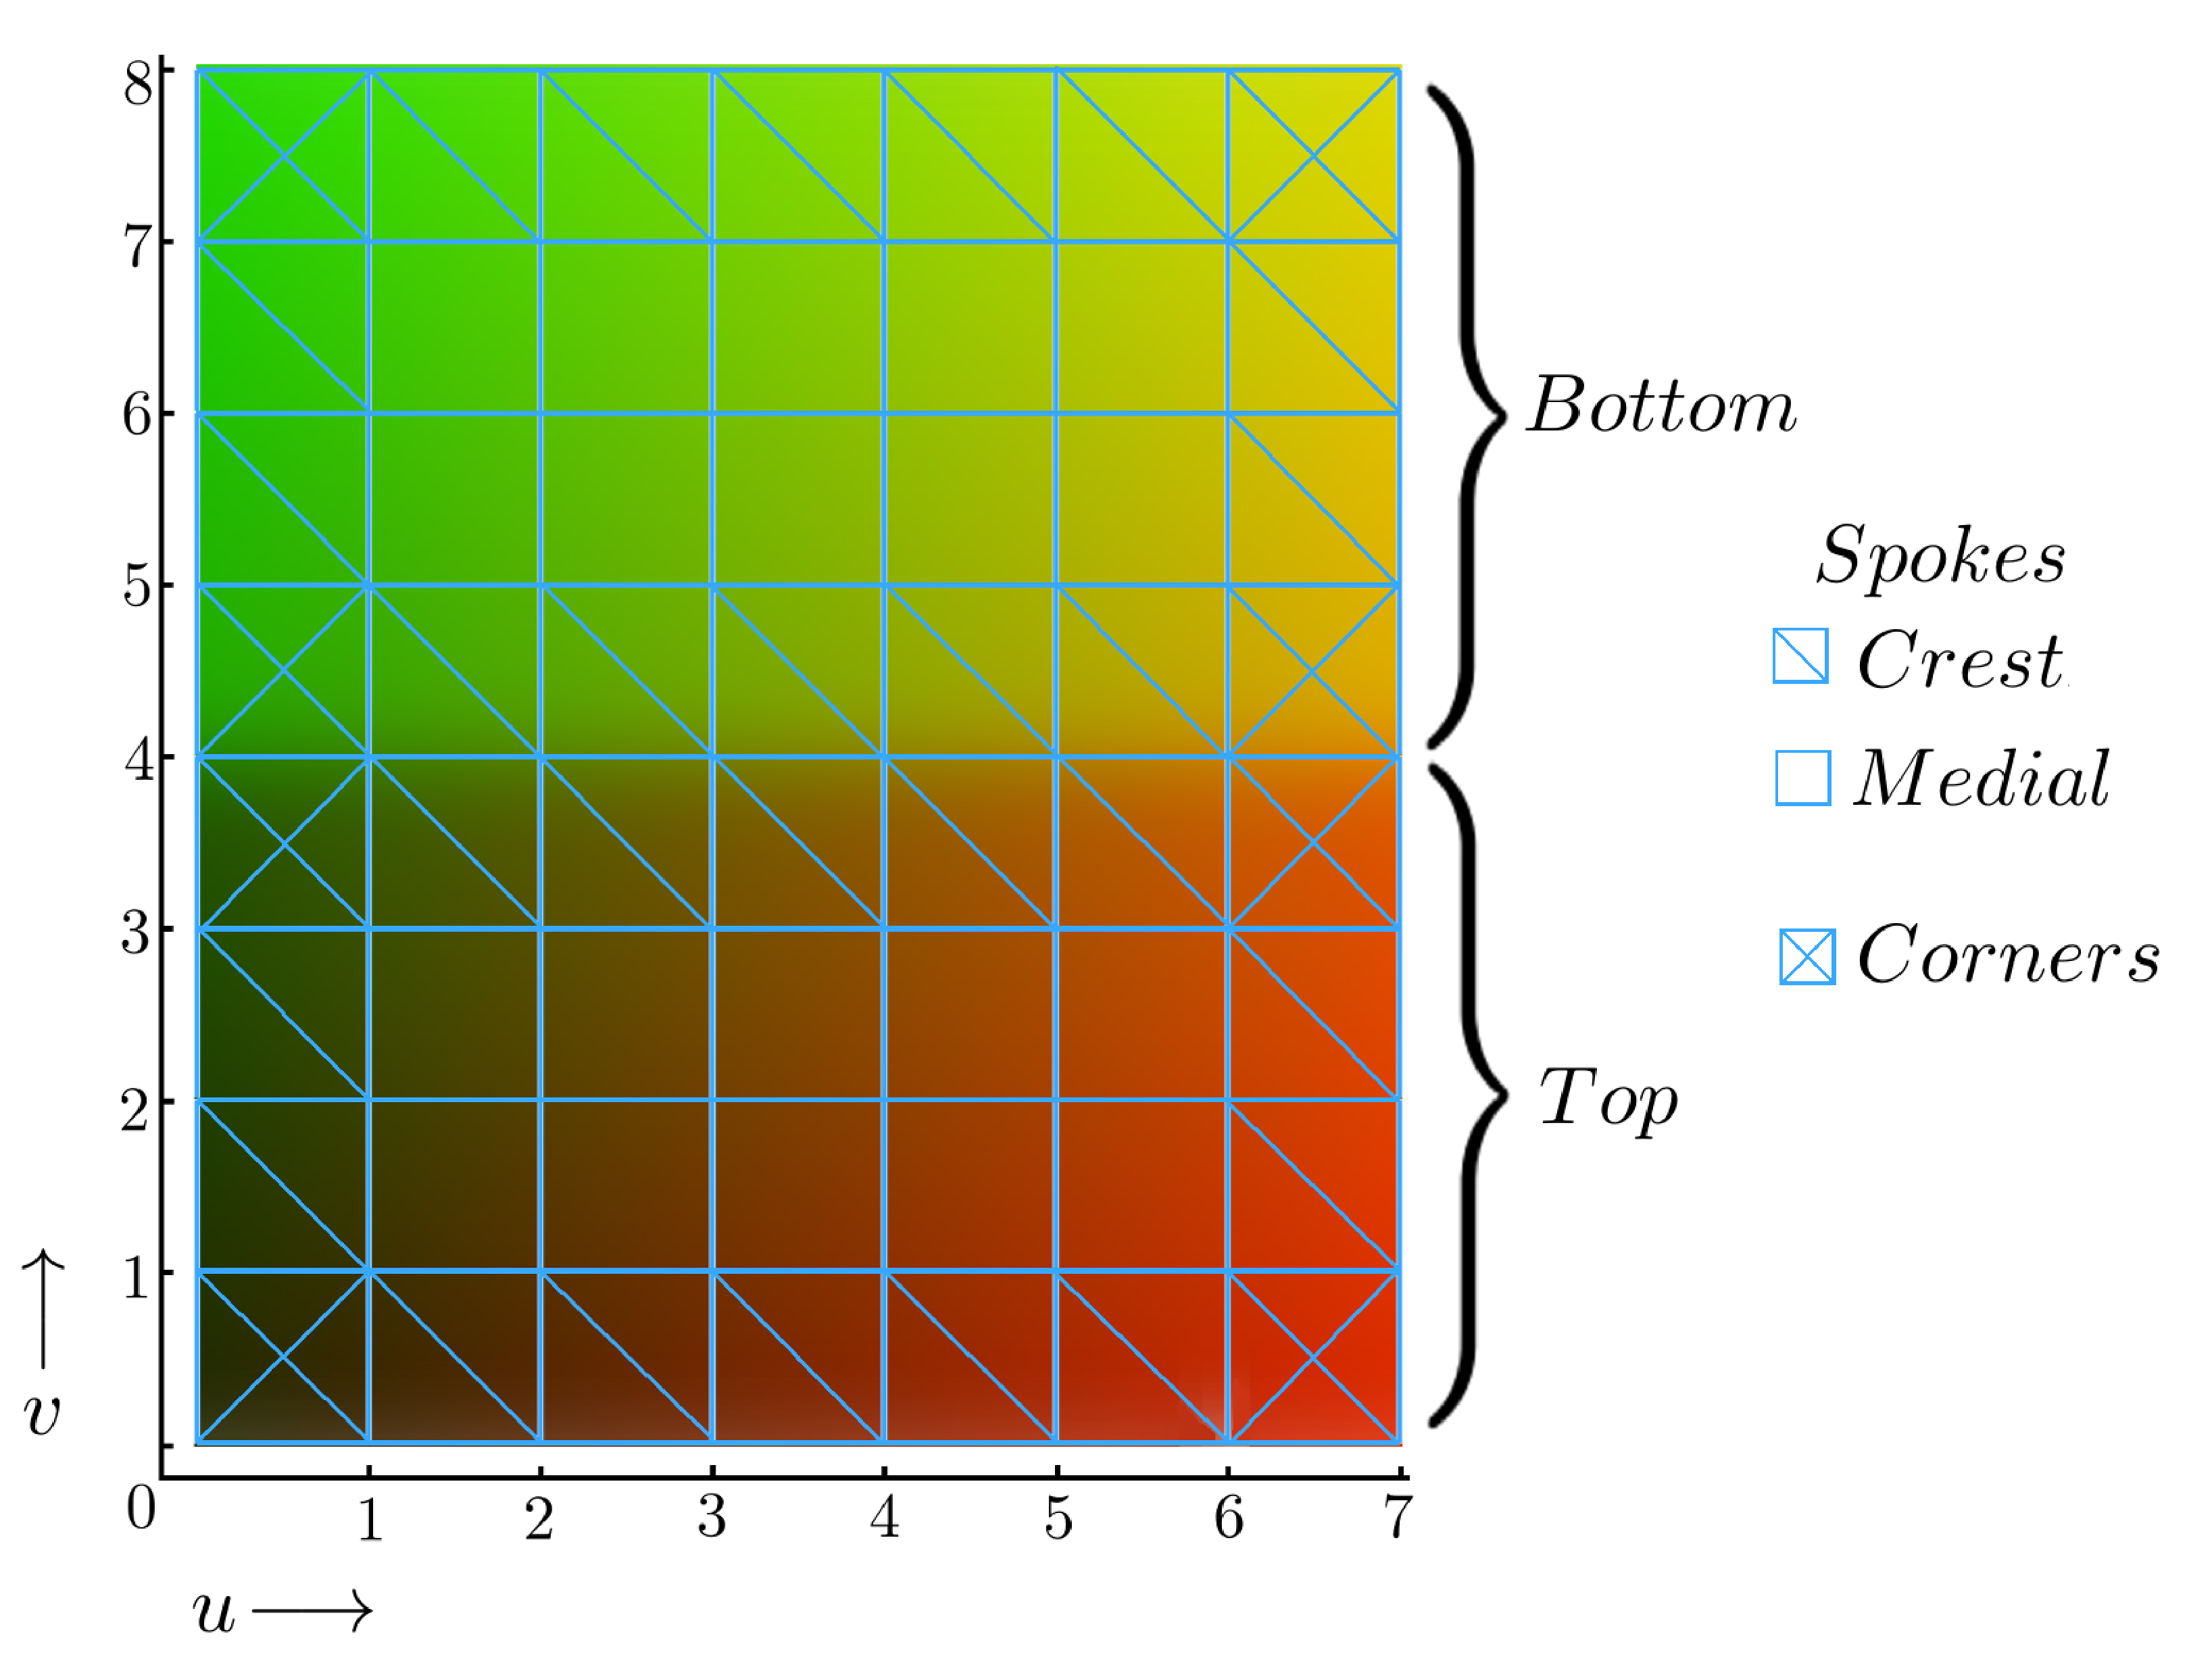
\epsfig{file = x2uMapGrid.eps, width = 13cm}
 \caption[Unfolding the s-rep.]{Unfolded s-rep of $6 \times 3$ atoms. Each intersection corresponds to a spoke in the s-rep,  
          the crest spokes repeat them selfs on the top and bottom sides. 
          The corners of the object are shown with the blue cross, 
          they also correspond to the 4 crest spokes that join top, bottom and connect the sides
          of the object. 
          Using this unfolded version of the MS we provide a unique $u, v$ value represented by the color gradient,
          the grid size is $(m + 1) \times 2\times(n + 1)$.
          }
 \label{fig:unfoldedSlab}  
\end{figure}

Figure \ref{fig:unfoldedSlab} shows a representation 
of the unique $(u, v$) coordinate given to 
every spoke in the object, they are represented by the color gradient
using red to for the $u$ direction and green for the $v$ direction. 
The blue color is used to represent the spoke length which is $\tau = 0$.

By means of the mechanisms described to interpolate the MS, top, bottom and crest spokes, 
a function $U2X(u, v, \tau) = [x, y, z] | (u, v, \tau) \in [0, 1])$ is designed to retrieve a position inside the 
object by querying $(u, v, \tau)$ coordinates.
This function is used to calculate the $X2U$ map. 

Figure \ref{fig:x2uMap} shows the $X2U$ map of the amygdala.

\begin{figure} 
 \centering  
  \subfigure[Top side]{
\epsfig{file = x2uMapTop.eps, width = 7cm}}
  \subfigure[Bottom side]{
\epsfig{file = x2uMapBottom.eps, width = 7cm}}
 \caption[X2U's map volume rendering.]{Volume rendering of an $X2U$ map showing both sides when $\tau = 1$}
 \label{fig:x2uMap}  
\end{figure} 


\section{Conclusions}
\label{sec:3dRepConclusion}

We have seen different types of approaches to model the boundaries of objects and produce statistics on 
their shape.
It has been shown that deformable models behave better 
and increase the accuracy of segmentation procedures or object recognition. They 
are less sensitive to noise and are more likely to find the global optimal object boundary.
Two major components in probabilistic deformable model methods are  
learning shape statistics and the segmentation of target images using the statistical probability distributions. 
There is still more improvement to be done 
at the training stage of the deformable model because this step requires 
too much user intervention and is time consuming. 

Besides surface modeling, a summary on 3D modeling techniques has been given. 
Those models are best suited to describe the internal features of 3D objects.
S-reps in particular are able to explain the continuum of space in an object, 
giving possibilities to include information into the model in a multi-scale fashion. 
The continuum of space described by the s-reps will be used  
to include the necessary parameters to perform MRI simulation. 

Furthermore, s-reps are suited to produce shape statistics with CPNS and can describe
shape variations with a few coefficients, a mean shape and eigenmodes of shape variation. 

The following chapter explains a novel methodology to 
fit s-reps to the brain cortex because they also support
foldability.
With the fitted structure a statistical analysis is conducted using CPNS
proving that s-reps are well suited to model 
complex structures. 

\newpage

